\chapter{Applications to Nonlinear Filtering} 
\label{ch:filtering}
% introduction to the chapter
Applications to nonlinear filtering was the main motivation behind the development of the $\gradTD$ learning algorithms in Chapters \ref{ch:diff_td} and \ref{ch:rkhs}. In this chapter, the problem of nonlinear filtering and the associated theory is described in detail in \Section{s:nl_filtering_intro}. A brief survey on approximations to the nonlinear filter, including the extended Kalman Filter (EKF) and particle filters, is provided in \Section{s:approx_nl_filter}. Feedback particle filter (FPF), which is the main focus of the dissertation is formally introduced in \Section{s:fpf}. A critical component of the FPF is the gain function, which is obtained as the gradient of the solution to Poisson's equation associated to the Langevin diffusion. A sketch of the derivation of the optimal gain function that guarantees asymptotic exactness of the FPF to the nonlinear filter is provided in \Appendix{a:fpf}. \anandspm{Should I skip this from the Appendix} Galerkin-based approximation methods and an algorithm based on approximating the Markov semigroup of the Langevin diffusion \cite{tagmeh16a}, which was developed in parallel research are presented in Sections \ref{s:galerkin} and \ref{s:coifman} respectively. Due to the gradient representation of the gain, $\gradTD$ algorithms described in \Chapter{ch:diff_td} and its RKHS based variants from \Chapter{ch:rkhs} offer a natural solution to approximating it. Two enhancements to the RKHS based $\gradTD$ learning algorithm are proposed to improve their performance in the FPF in \Section{s:fpf_rkhs_improvements}. Finally, \Section{s:fpf_numerics} contains a number of numerical experiments that compare the performance of the various algorithms for gain approximation and for filtering problems.  

\section{Introduction to Nonlinear Filtering} 
\label{s:nl_filtering_intro}
A preliminary introduction to nonlinear filtering was provided in \Chapter{ch:intro}. A schematic diagram of a state estimator appears in \Fig{Fig:state_estimator}. Our goal in this section is to make things more precise through a more formal description of the problem. First, we begin with a motivating application. Nonlinear filtering has its origins in tracking problems in satellite and aircraft navigation. The key goal of filtering is to obtain recursive estimates of the state of a stochastic dynamical system based on partial noisy observations. A typical example in a tracking application is the simultaneous estimation of position and velocity of a moving target. Here, position and velocity of the target constitute the state of the system and the observations are modeled as nonlinear functions of the state made in the presence of noise. More recently, filtering has found applications in diverse areas such as machine learning \cite{bishop06}, queueing networks, mathematical finance \cite{brihan08} and data assimilation problems for weather forecasting \cite{eve94}. 

A filtering problem can be formulated in continuous or discrete-time and continuous or finite state-space depending on the application of interest. 
The simplest dynamical model for filtering in discrete-time and state space is the Hidden Markov Model (HMM). In this dissertation however, we are primarily interested in a filtering problem in continuous-time with states evolving on a Euclidean space. For simplicity, let us restrict ourselves to the scalar filtering problem:
\begin{equation}
\begin{aligned}
\text{State model}: \quad & \ud X_t&=a(X_t) \ud t +\sigma_{B}\ud B_t,\\
\text{Observation model}: \quad & \ud Z_t&=c(X_t) \ud t + \sigma_{W}\ud W_t,
\label{e:fpf_cts_filtering}
\end{aligned}
\end{equation}
where $\bfmX=\{X_t\}$ is the scalar state process, $\bfmZ=\{Z_t\}$ is the scalar observation process, $a$ and $c$ are $C^{1}$ functions, and  $\bfmB= \{B_t\}$,  $\bfmW = \{W_t\}$ are mutually independent standard Brownian motions.   The state model describes the evolution of the hidden state of the system. The uncertainties in the state model and the external disturbances that affect the dynamics are modeled as the state noise term $\bfmB$. Indirect observations, in the form of nonlinear functions of the state corrupted by noise $\bfmW$ are available via the observation model. The goal of the filtering problem is to approximate the posterior density 
$\pr^*_t$  of $X_t$,
given the past observation history $\clZ_t\eqdef\sigma(Z_s:s\leq t)$. For any measurable set $A \subset \Re$, the posterior density $\pr^*_t$ is defined as, 
\begin{equation}
\int_A \pr^*_t(x) \ud x \eqdef \Prob\{ X_t \in A \mid \clZ_t\}.
\label{e:fpf_posterior_exact}
\end{equation}


A huge body of literature has been devoted to the study of such problems. 
The theory of nonlinear filtering has been described in \cite{kal80, baicri08}. A more accessible derivation of the nonlinear filter, from a change of measure standpoint is provided in \cite{kutsurpfi19}. In this section, without going into a lot of detail, we state some of the important results.
\subsection{Zakai and Kushner-Stratonovich equations}
Zakai's equation \cite{zak69} and Kushner-Stratonovich (K-S) \cite{kus67, str60} equations are the key results in this area. 
The Kushner-Stratonovich equation provides a stochastic PDE describing the evolution of $\pr^*_t$:
\begin{equation}
\ud \pr^*_t(x) = \generate^\dagger \pr^*_t(x) \ud t + \frac{1}{\sigma^2_W} (c(x) - \hat{c}_t) (\ud Z_t - \hat{c}_t\ud t) \pr^*_t(x),
\label{e:fpf_kushner_stratonovich}
\end{equation}
where $\generate^\dagger \pr \eqdef - (d(\pr a) / dx) + (\sigma^2_B/2) (d^2 \pr /d x^2)$ is the adjoint operator to the differential generator of the SDE describing the state model in \eqref{e:fpf_cts_filtering} and $\hac_t \eqdef \int c(x) \pr^*_t(x) dt$. 
For a nonlinear observation function $c(x)$, a moment closure problem arises in the K-S equation and hence, it cannot generally be reduced to stochastic PDEs so that they could be numerically integrated. In some cases, it is convenient to use the Zakai's equation, which is a linear stochastic PDE that describes the evolution of the unnormalized posterior density $\tilde{\pr}^*_t$: 
\begin{equation}
\ud \tilde{\pr}^*_t(x) = \generate^\dagger \tilde{\pr}^*_t(x) \ud t + \frac{1}{\sigma^2_W}  c(x) \ud Z_t \tilde{\pr}^*_t(x), 
\label{e:fpf_zakai}
\end{equation}
\anandspm{need the definition of $\generate^\dagger$. Is it the adjoint to the differential generator?}

\subsection{Kalman-Bucy filter}
Solution to the \cref{e:fpf_kushner_stratonovich,e:fpf_zakai} are in general, infinite dimensional. In the special case where the functions $a(x)$ and $c(x)$ are linear, i.e. $a(x) = Ax$ and $c(x) = Cx$ and the prior distribution $\pr_0$ is Gaussian, it is guaranteed that the posterior density $\pr^*_t$ also remains Gaussian for all $t$. A closed-form solution can be obtained to the filtering problem in this case. The posterior density $\pr^*_t$ is completely characterized by the conditional mean $\mu_t$ and the state covariance $\Sigma_t$. The optimal filter is given by the classical Kalman-Bucy filter \cite{kal64}, which is described by the set of \cref{e:fpf_kalman_mu,e:fpf_kalman_sigma}, for a scalar system:
\begin{align}
\text{Conditional mean:} \quad \ud \mu_t & = A \mu_t \ud t + \underbrace{\frac{\Sigma_t C}{\sigma^2_W}}_{\text{Kalman gain}} ( \ud Z_t - C \mu_t \ud t), 
\label{e:fpf_kalman_mu} \\
\text{State covariance:}  \quad  \frac{\ud}{\ud t} \Sigma_t &= 2 A \Sigma_t + \sigma^2_B - \frac{\Sigma^2_t C^2}{\sigma^2_W}. 
\label{e:fpf_kalman_sigma}
\end{align}
Here, the conditional mean $\mu_t$ evolves according to the SDE in \eqref{e:fpf_kalman_mu} and \eqref{e:fpf_kalman_sigma} is an ODE called the continuous-time Riccati equation. The state covariance $\Sigma_t$ evolves independent of the observations $Z_t$ and the conditional mean $\mu_t$ and as a result, it can be solved offline.  
The term $\frac{\Sigma_t C}{\sigma^2_W}$ is called the Kalman gain, denoted as $\Kkal$. 
\section{Approximations to the Nonlinear Filter}
\label{s:approx_nl_filter}
In a general nonlinear setting, excepting special cases like the Bene\v{s} filter \cite{ben81}, the optimal nonlinear filter cannot expressed in terms of a finite set of parameters. \Cref{e:fpf_kushner_stratonovich,e:fpf_zakai} show that the posterior density can be computed in a recursive fashion. This leads to the development of discretization schemes to approximate the nonlinear filter. However, numerical approximations to the solution of the K-S equation using an Euler-type discretization are not accurate or robust. 

As noted in \Section{s:filtering}, typically a filtering problem can be separated into two steps - prediction step, where the posterior density $\pr^*_t$ at time $t$ is propagated according to the state model, without accounting for the current observations, and the correction step, where the estimates are corrected after receiving the latest observations. As the state dimension increases, numerical solutions to both these steps become prohibitively expensive and approximate solutions are sought. Approaches to approximating the prediction step and the correction step can be chosen independently and then combined. In a broad sense, two approaches can be taken, one where an exact solution is obtained under the assumptions of linearity and another, where a finite-dimensional approximation of the Kushner-Stratonovich equation is used. Budhiraja et al. in \cite{budchelee07} provide a comprehensive survey of approximation techniques for nonlinear filtering, with a particular focus on particle filtering based algorithms. A tutorial on a number of variants of particle filtering methods, particularly in the discrete-time setting is given in \cite{arumasgorcla02}.
\subsection{Extended Kalman filter}
\label{s:ekf}
Extended Kalman filter (EKF) \cite{jaz70} is based on the principle of local linearization of the state and observation models around the mean $\mu_t$. Consequently, the resulting posterior densities are approximated as Gaussians. In the EKF, the conditional mean and state covariance estimates for the system in \eqref{e:fpf_cts_filtering} are governed by the following equations: 
\begin{align}
\ud \mu_t = a(\mu_t) \ud t + \frac{\Sigma_t C(\mu_t)}{\Sigma^2_W} (\ud Z_t - c(\mu_t) \ud t), \\
\frac{\ud}{\ud t} \Sigma_t = 2 A(\mu_t) \Sigma_t  + \sigma^2_B - \frac{\Sigma^2_t C^2(\mu_t)}{\sigma^2_W}, 
\label{e:fpf_ekf}
\end{align}
where $A = \frac{d a}{dx}$ and $C = \frac{d c}{dx}$. In higher dimensional state spaces, $A$ and $C$ are the Jacobian matrices. These are fairly easy to implement for moderate state dimensions. The performance of the EKF deteriorates if the state and observation models deviate significantly from linearity or if the noise variances are high and as a result, they suffer from severe divergence and instability problems. Furthermore, the EKF fails to capture the multi-modal features of the posterior distribution.
\subsection{Particle filters}
\label{e:fpf_particle}
Particle filters are Monte Carlo based approximations to the nonlinear filter \cite{doucet2000sequential}. \anand{check this reference} They belong to the second category mentioned, wherein without relying on the linearization of dynamics, the posterior is approximated using a finite number of samples called particles. They are based on the idea of sequential importance sampling (SIS). Although, the discrete-time variant of the filter is more common, the derivation of the continuous-time particle filter is provided in \cite{kutsurpfi19}. The basic idea is this: a large number of particles $\{X^i_0\}$ drawn independently from the same prior distribution $\pr^*_0$ are propagated through time according to the state model \eqref{e:fpf_cts_filtering}. Each particle is associated with an importance weight. Initialized with equal weights, the weight corresponding to each particle is updated based on the observations as follows:
\begin{equation}
% w^i_t  = \frac{1}{W_t} \exp \Bigl[ \int_0^t \frac{c(X^i_s)}{\sigma^2_W} dZ_s - \frac{1}{2} \int_0^t \frac{c^2(X^i_s)}{\sigma^2_W} ds\Bigr],
\ud w^i_t = w^i_t  \Bigl(\frac{1}{\sigma^2_W} \Bigr) (c(X^i_t)  - \bar{c}_t ) (\ud Z_t - \bar{c}_t \ud t),
\label{e:fpf_particle_wt}
\end{equation}
where $\bar{c}_t \eqdef \sum_{i=1}^N w^i_t c(X^i_t)$. The particle locations $\{X^i_t\}$ along with the importance weights $\{w^i_t\}$ are used to come up with an empirical estimate of the posterior distribution as:
\begin{equation}
\pr^*_t(x) \approx \pr^{(N)}_t(x) = \sum_{i=1}^N w^i_t \delta(x -X^i_t),
\label{e:fpf_particle_empirical}
\end{equation}
where $\delta$ is the Dirac-delta function. 

Particle filters are easy to implement and are ideally suited for a parallel computing architecture. The accuracy of the estimates improves as $N$ increases. They do not require linearization of the model or discretization of the filter SDEs and are often seen to outperform the EKF in highly nonlinear examples. However, they are known to suffer from particle degeneracy, where after a few iterations, only a handful of particles remain with significant weights, thus reducing the effective sample size. A proposed remedy is frequent resampling of particles when the effective particle size falls below a predetermined threshold. After the resampling step, the importance weights of the new particles are reinitialized to be equal. Certain resampling schemes may again result in loss of diversity or sample impoverishment due to the replication of the same particles. A host of resampling schemes aimed at resolving these issues is presented in \cite{budchelee07, arumasgorcla02}.
 
\section{Feedback Particle Filter (FPF)}
\label{s:fpf}
In this section, we introduce the feedback particle filter (FPF), which is the preferred approximation of the nonlinear filter in this dissertation. In \Section{s:approx_nl_filter}, several approximations to the nonlinear filter, including the EKF and the particle filter were presented. In addition to providing an overview of such techniques, one of the purposes behind giving a detailed exposition was to enable us to compare and contrast the similarities (and dissimilarities) of these techniques with the FPF.  

FPF was first introduced in \cite{yanmehmey11} as an alternative approach to particle filtering, inspired by mean-field optimal control techniques. Along the lines of particle filtering, the FPF is constructed as a collection of $N$ particles,  each of which evolves according to a stochastic differential equation (SDE). The state evolution of the $i^\text{th}$ particle at time $t$, denoted $X_t^i$ mimics that of the state model:
\begin{equation}
\ud X^i_t = \underbrace{a(X^i_t) \ud t + \sigma_B \ud B^i_t}_{\text{Prediction}} + \underbrace{\ud U^i_t}_{\text{Correction}},
%\kFPF_t(X^i_t) \circ \underbrace{(\ud Z_t -\half[c(X^i_t) + \hac_t]\ud t)}_{\ud I_t}\, ,
\label{e:fpf_nonlin_intro}
\end{equation}
in which each $\bfmB^i$ is a standard Brownian motion.  The initial conditions $\{X^i_0: 1 \le i\le N\}$ are assumed i.i.d., with common prior distribution $ \pr_0^*$. The primitives $\bfmB^i$ and $\{X^j_0: j\ge 1\}$ are mutually independent, and also independent of $(\bfmX,\bfmZ)$. The particles are all coupled via the control input term $U_t^i$ corresponding to the $i^{\text{th}}$ particle.  The conditional distribution of a particle $X^i_t$ given $\clZ_t$ is given by:
\begin{equation}
\int_A \pr_t(x) \ud x = P\{X^i_t \in A \mid \clZ_t\},
\label{e:fpf_posterior}
\end{equation}
and an empirical approximation of $\pr_t$ is obtained as:
\begin{equation}
\pr^{(N)}_t(A) \eqdef \sum_{i=1}^N \ind_A\{X^i_t \in A\},
\label{e:fpf_emp_posterior}
\end{equation}
where $A \in \clB$ (Borel measurable subsets of $\Re$) measurable set in $\Re$. The particles are conditionally independent given the observations, so that for large $N$,  the approximation $\pr_t^{(N)}\sim \pr_t$ holds in a weak sense.    \anandspm{This was $\pr^*_t$ before, but I guess it should be this.}
%, and $\hac_t := \Expect[c(X_t^i)\mid \clZ_t]$


The main difference in \eqref{e:fpf_emp_posterior} compared to the estimate in \eqref{e:fpf_particle_empirical} is that all the particles are weighted equally in the FPF. Such unweighted approaches hold the promise of avoiding the resampling step and overcoming the curse of dimensionality that the standard particle filter suffers. Similar unweighted particle filter approaches were proposed in \cite{mitnew04,crixio05}. Daum et al. discuss the limitations of the conventional particle filter and present a filtering scheme for the continuous-discrete time case, called the information flow filter. A detailed comparison of the FPF with the information flow filter is provided in \cite{taoyang_acc14}. Neural particle filter (NPF), another unweighted approach is presented in \cite{kutsursprpfi17}. A more extensive list of filtering techniques based on interacting particle systems can be found in \cite{yanlaumehmey16}. The FPF has found success in applications such as physical activity recognition \cite{tilhsimeh12, tilmehmey12a},  satellite navigation \cite{bergro16, berntorp15} etc. 

It may also be noted that prediction and correction operations are performed in a single step in \eqref{e:fpf_nonlin_intro}. The correction step is implemented via the control input term $U^i_t$. For each $i$, the control input $\bfmU^i$ is constructed so that for any $t$ and any $A\in\clB $,
\[
\Prob\{ X^i_t \in A \mid \clZ_t\} 
=
\Prob\{ X_t \in A \mid \clZ_t\}
=
\int_A \pr^*_t(x) \ud x.
\] 
The problem of choosing the optimal $U^i_t$ such that the posterior density $\pr$ coincides with the true posterior $\pr^*_t$ is cast as an optimal control problem in \cite{yanmehmey11,yanmehmey13}. The Kullback-Leibler divergence between the true posterior $\pr^*$ and the FPF mean-field estimate $\pr$ is used as the cost function. An explicit formula for $U^i_t$, derived in \cite{yanmehmey13} and it is used to control the dynamics of the $i^{\text{th}}$ particle:
\begin{equation}
\ud X^i_t = a(X^i_t) \ud t + \sigma_B \ud B^i_t + \underbrace{\kFPF_t(X^i_t) \ud I^i_t + \Omega(X^i_t,t) \ud t}_{\text{optimal control input }U^i_t}, 
\label{e:fpf_optimal_input}
\end{equation} 
where $\Omega(x,t)\eqdef \frac{1}{2} \sigma^2_W \kFPF_t(x) \frac{\partial \kFPF_t(x)}{\partial x}$ and $\{I^i_t :  t \geq 0 \}$ is analogous to the innovations process corresponding to the $i^{\text{th}}$ particle,
\begin{equation}
\ud I^i_t \eqdef \ud Z_t - \frac{1}{2} (c(X^i_t) + \hat{c}_t) \ud t,
\label{e:fpf_innovations}
\end{equation}
with $\hat{c}_t \eqdef \Expect[c(X^i_t)\mid \clZ_t] = \int c(x) \pr_t(x)\, dx$ and approximated using $\hat{c}^{(N)}_t  \eqdef \frac{1}{N} \sum_{i=1}^N c(X^i_t)$. The filter is expressed in the Stratonovich form as:
\begin{equation}
\ud X^i_t =  a(X^i_t) \ud t + \sigma_B \ud B^i_t + \kFPF_t(X^i_t) \circ \ud I^i_t,
\label{e:fpf_stratonovich}
\end{equation}
where, the symbol ``$\circ$'' indicates  that the SDE is in Stratonovich form. The main subject of interest in this dissertation is the gain function $\kFPF_t$, that multiplies the innovations term $I_t$ in \eqref{e:fpf_stratonovich}. A detailed description of the gain function is provided next in \Section{s:fpf_gain}.
% \anand{Include block diagrams comparing FPF and KF}
\subsection{FPF gain function}
\label{s:fpf_gain}
It is evident from \eqref{e:fpf_stratonovich}, that the FPF exhibits a gain $\times$ innovation error structure that is a hallmark feature of the Kalman-Bucy filter. This feedback control structure was also present in the K-S equation \eqref{e:fpf_kushner_stratonovich} describing the nonlinear filter, but conspicuously absent in the standard formulation of the particle filter \anand{bootstrap PF?}. The FPF restores this feedback structure, which contributes to the robustness of the filter via the self-correcting property.  The block diagrams in \Fig{fig:fpf_kalman} illustrate the similarity in structure of the FPF with the Kalman filter. However, unlike the Kalman-Bucy filter where the gain is a constant, the FPF gain function $\kFPF_t$ depends on the state $X_t$. For a linear-Gaussian system, the optimal gain has been shown to coincide with the Kalman gain. 
\begin{figure}[htbp]
	\centering
		\includegraphics[width = 7in]{images/Chap4_FPF_Kalman}
		\caption{Schematic block diagrams comparing the Kalman filter and the feedback particle filter (FPF) \cite{yanmehmey13}}
		\label{fig:fpf_kalman}
\end{figure}

To implement the FPF, the gain function $\kFPF_t$ needs to be computed for each $t$. To simplify notation, consider a fixed time $t\ge 0$,  and suppress dependency on $t$.  In particular, let $\kFPF$ denote the gain function that appears as  $ \kFPF_t$  in \eqref{e:fpf_nonlin_intro},  and let $\pr$ denote the conditional density $\pr_t$. It has been proved in \cite{yanmehmey13} that the optimal gain is obtained as the solution to the following Euler-Lagrange boundary value problem (EL-BVP):
\begin{equation}
\begin{aligned}
%-\frac{\partial}{\partial x} \Bigl( \frac{1}{\pr(x)} \frac{\partial}{\partial x} \{\pr(x) \kFPF(x)\}\Bigr) = \frac{1}{\sigma_W^2} c'(x), 
\nabla \cdot \Bigl(\frac{1}{\pr(x)} \nabla (\pr(x) \kFPF(x))\Bigr) &= - \frac{1}{\sigma^2_W} \nabla c, \\
\lim_{x \to \infty} \kFPF(x) \pr(x) = 0.
\label{e:fpf_el_bvp}
\end{aligned}
\end{equation}% where $c'(x) = \frac{\partial c }{\partial x}$. 
Denoting $\pot=-\log(\pr)\in C^1$, it is easy to show by simple integration that the EL-BVP in \eqref{e:fpf_el_bvp} can be equivalently characterized in the standard form of Poisson's equation for the Langevin diffusion \eqref{e:fpf_poissons}.
\begin{equation}
\generate h = -\nabla \pot \cdot \nabla h + \Delta h  = -\tilc, \qquad \tilc = c - \int c(x) \pr(x)\, \ud x, 
\label{e:fpf_poissons}
\end{equation}
where the gain $\kFPF$ coincides with the gradient of $h$:
\begin{equation}
\kFPF (x) = \nabla h(x)\, ,  \quad x\in\state\, .
\label{e:fpf_k_gradient}
\end{equation}
The formula for the gain is thus obtained via a solution to the Poisson's equation:
Assuming $\nabla U$ is globally Lipschitz continuous, and under some regularity conditions on $c$, the solution $h$ and its gradient exists, as discussed in \Chapter{ch:diff_td}. In the remainder, it is assumed that these regularity conditions are satisfied and that the gain $\kFPF$ exists and is unique. Theorem 3.3 in \cite{yanmehmey13} states that provided the prior densities match, i.e. $\pr^*_0(x) = \pr_0(x)$, the FPF in \eqref{e:fpf_stratonovich} with the gain $\kFPF$ obtained as a solution to \eqref{e:fpf_el_bvp} is consistent with the optimal nonlinear filter \eqref{e:fpf_kushner_stratonovich}, i.e.
\begin{equation}
\pr_t(x) = \pr^*_t(x). 
\end{equation}
An estimate of $\pr_t$ given by the empirical distribution of the particles $\pr^{(N)}_t$ approximates $\pr^*_t$ as $N \to \infty$. 
\section{FPF Gain Approximation}
The major challenge in the implementation of the FPF is the computation of the gain function. The exact computation of $\kFPF$ is intractable outside of these particular cases. 
\begin{romannum}
\item When $\pot$ is quadratic and $c$ is linear,  then $\kFPF$ is a constant independent of $x$, and can be interpreted as a Kalman gain \cite{yanlaumehmey13}. 

\item In the general scalar case, when $d=1$, $\kFPF$ has an explicit solution:
\begin{equation}
\kFPF(x) = - \frac{1}{\pr(x)} \int_{-\infty}^{x} (c(y) - \hat{c}) \pr(y) \ud y.
\label{e:fpf_gain_1d}
\end{equation}
\end{romannum}

This motivates the use of approximation techniques to obtain an estimate of $\kFPF$ that is optimal in some meaningful metric. In the first part of this section, we discuss Galerkin-based gain approximation algorithms. An algorithm based on approximation of the transition kernel of the Langevin diffusion was developed in parallel research by Taghvaei et al. \cite{tagmeh16} and error analysis of this method was studied in \cite{tagmehmey17}. This algorithm has been used in this dissertation as an important benchmark for comparing the performance in numerical simulations. A short review is provided in \Section{s:coifman}. 

As motivated in Chapters \ref{ch:diff_td} and \ref{ch:rkhs}, approximation algorithms based on $\gradTD$ learning form the core topic of this dissertation. It is evident from \eqref{e:fpf_k_gradient}, that the objective function used in \eqref{e:diff_td_gradTD_norm_error} suits the objective of approximating the gain $\kFPF$ very well:
\begin{equation}
\| \nabla h - \nabla h^\param \|^2_{L^2} = \| \kFPF - \kFPF_\param \|^2_{L^2}.
\end{equation}
Thus, $\gradTD$ learning algorithms can be directly applied for gain approximation. Two refinements of the RKHS based $\gradTD$ learning algorithm to enable online gain estimation, are proposed in \Section{s:fpf_rkhs_improvements}.

\subsection{Galerkin-based methods}
\label{s:galerkin}
Galerkin-based algorithms are a result of a weak formulation of the EL-BVP \eqref{e:fpf_el_bvp}. A function $h$ is called a weak solution to the Poisson's equation \eqref{e:fpf_el_bvp} if
\begin{equation}
\int \nabla h (x) \cdot \nabla \test(x)  \pr(x) dx = \int \tilc(x) \test(x) \pr(x) dx, \forall \test \in H^0_1,
\label{e:fpf_galerkin}
\end{equation}\anand{Need to verify $H^0_1$.}
where $\test(x)$ are called test functions. This formulation is called a Galerkin relaxation. \anand{reference?}
A finite dimensional solution to \eqref{e:fpf_galerkin} is obtained by choosing an $\ell$-dimensional  function class
$\clH  \eqdef \{h^\param : \param \in \Re^\ell\}$ to approximate $h$ and a collection of $\ell$ test functions $\{\test_j\}_{j=1}^{\ell}$. In prior work \cite{yanmehmey13,yanlaumehmey16}, $\clH$ is considered to be a linearly parameterized family of functions of the form $h^\param \eqdef \sum_{j=1}^{\ell}\param_{j}\basis_{j} $, where $\{\basis_j\}$ are called the basis functions.  It is assumed that each $\basis_j$ is continuously differentiable,  with gradient denoted   $\gradbasis_{j} $.
 These   functions are used to define the approximation of the filter gain
\begin{equation}
K_\param = \nabla h^\param= \sum_{j=1}^{\ell}\param_{j}\gradbasis_{j}.
\label{e:fpf_basis_galerkin}
\end{equation}
Then, the Galerkin relaxation of Poisson's equation \eqref{e:fpf_galerkin} is defined to be the set of $\ell$ equations in the parameter $\param$. A particular case is when the set of test functions and basis functions chosen are the same. The solution $\param$ in this case is given by:
\begin{equation}
\begin{aligned}
\param & = M^{-1} b, \\
\text{where}&,\\ 
M \eqdef \langle \gradbasis, &\gradbasis \rangle, \quad b \eqdef \langle \tilc, \basis \rangle.
\label{e:fpf_test_basis}
\end{aligned}
\end{equation}
Empirical estimates for $M$ and $b$ can be computed using particles. If the particles are distributed according to $\pr$, then the solution \eqref{e:fpf_test_basis} is the same as the optimal solution obtained using $\gradTD$ learning for a linear parameterization \eqref{e:diff_td_gradTD_theta}. This is a matter of coincidence rather than design, and in general, Galerkin formulations do not result in norm minimization. 

Another Galerkin formulation is obtained in terms of the Bellman error. Recall that the FPF gain is the derivative of the solution to Poisson's equation \eqref{e:fpf_poissons}. For the linear parameterization, the following formulation results in $\ell$ linear equations as before:
\begin{equation}
\begin{aligned}
0 &= \langle \underbrace{\clD h^\param+\tilc}_{\text{Bellman Error}}, \test_{j} \rangle \\
&= \int (-\nabla U(x) \cdot \nabla h^\param(x)+ \Delta h^\param(x)+\tilc (x))\test_{j}(x) \ud x,  \qquad  1\leq j \leq \ell.
\end{aligned}
\label{e:fpf_galerkin_be}
\end{equation}

% \anand{Provide a gain approx in algorithmx format}
A commonly used estimate for $\kFPF$ that is easily computable is the constant gain approximation, denoted as $\kFPF^*$. This is obtained by choosing $\{\basis_j(x) = x_j\}_{j=1}^d$ as the basis and test functions in the Galerkin relaxation. This results in  $M = I_{d}$ and,
\begin{align}
\hakFPF^*_j \eqdef b & = \langle \tilc , x_j \rangle \\ 
& \approx \frac{1}{N} \sum_{i=1}^N [ c(x^i_j) - \hac ]x^i_j, \qquad 1 \leq j \leq d,
\label{e:fpf_gain_const_approx}
\end{align}
where $\hakFPF^*_j$ is the $j^{th}$ component of the gain.
Alternately, the constant gain can also be interpreted as the minimizer of 
  \begin{equation}
  \hakFPF^* \eqdef \argmin_{\hakFPF \in \Re^d} \| \kFPF - \hakFPF \|^2_{L^{2}}
  \label{e:fpf_const}
  \end{equation}
  where the minimum is over deterministic vectors. The solution is evidently the mean,  $\hakFPF^* = \Expect[\kFPF]$.
The proof of the representation \eqref{e:fpf_gain_const_approx} can also be obtained by applying \eqref{e:diff_td_gradDual}: 
\[
\hakFPF^*_ j =  \langle \kFPF^* ,e_j \rangle_{L^2}
=
\langle \tilc ,\psi_j \rangle_{L^2}\,, \qquad 1\le j\le d\,,
\]
where $\{e_j\}$ are the standard basis elements in $\Re^d$. This approximation has been successfully tested in \cite{tilghiomeh13}. The constant gain is an important component of the refinements to the RKHS based $\gradTD$ algorithm proposed in \Section{s:fpf_rkhs_improvements}.

The Galerkin methods provide a good algorithmic framework for approximating the gain. However, in general it is not easy to obtain performance guarantees. In this dissertation, we obtain approximations by solving  the minimum norm problem \eqref{e:diff_td_gradTD_norm_error} using $\nabla$-TD learning.  Under general conditions we can be assured that the approximation is the minimum-norm optimal solution.   

\subsection{Markov semigroup approximation}
\label{s:coifman}
In this section, a very concise overview of the Markov semigroup approximation for the FPF gain function is provided. The algorithm was initially presented in \cite{tagmeh16}, followed by error analysis in \cite{tagmehmey17}. While the approach is entirely different, it is likely that concepts from this concurrent work can provide valuable insights to design an improved solution that combines the merits of both the approaches. 

The algorithm is based on a semigroup formulation of the Poisson's equation for Langevin diffusion \eqref{e:diff_td_poissons}. The function $h$ can be expressed as the solution to the following fixed-point equation:
\begin{equation}
h = P_\epsilon h + \int_0^\epsilon P_s (h - \hah) \ud s,
\end{equation}
where $P_\epsilon$ refers to the transition semigroup of the Langevin diffusion, defined in \eqref{e:diff_td_langevin_semigroup}. The main step is the use of an approximate semigroup $\text{T}$ in place of $P_\epsilon$.
An empirical solution to the fixed-point equation at the particle locations is obtained through successive approximation. The gain is subsequently obtained by taking the gradient.  A summary of the algorithm to approximate the gain for a fixed time $t$ is tabulated in \Algorithm{alg:coifman}:
\begin{algorithm}{Markov semigroup gain function approximation algorithm}
\begin{algorithmic}[1]
	%\caption{Markov semigroup algorithm for gain function approximation}
	\Require $\{x^i\}_{i=1}^N, \{c(x^i)\}_{i=1}^N, h_{prev}, \epsilon, L$.
	\Ensure $\{\kFPF_i\}_{i=1}^N$
	\State Calculate $\Kern_{ij} = \exp(-\|x^i - x^j\|^2/ 4\epsilon)$ for $i,j = 1$ to $N$  \Comment{Gaussian kernel}
	\State Calculate $\kappa_{ij} = \frac{\Kern_{ij}}{\sqrt{\sum_k \Kern_{ik}}\sqrt{\sum_k \Kern_{jk}}}$ for $i,j =1$ to $N$
	\State Calculate $d_i = \sum_j \kappa_{ij}$ for $i=1$ to $N$
	\State Calculate $\text{T}_{ij} = \frac{\kappa_{ij}}{d_i}$ for $i,j = 1$ to $N$ \Comment{Approximation of the Markov kernel for Langevin diffusion}
	\State Calculate $\pi_i = \frac{d_i}{\sum_j d_j}$ for $i=1$ to $N$
	\State Calculate $ \hac = \sum_{i = 1}^N \pi_i c(x^i)$
	\State Initialize $h =h_{prev}$
		 \For{$t =1$ to $L$}
		 \State $h_i = \sum_{j=1}^N \text{T}_{ij} h_j + \epsilon (c - \hac)$ for $i=1$ to $N$ \Comment{Successive approximation}
		\EndFor
	\State Calculate $r_i = h_i + \epsilon c_i$ for $i=1$ to $N$
	\State Calculate $s_{ij} = \frac{1}{2\epsilon} \text{T}_{ij} (r_j - \sum_{k=1}^N \text{T}_{ik} r_k)$ for $i,j=1$ to $N$ 
	\State Calulate $\kFPF_i  = \sum_j s_{ij} x^j$ for $i =1$ to $N$ \Comment{FPF gain function approximation}
	\label{alg:coifman}
\end{algorithmic}
\end{algorithm}

Similar to the RKHS-based $\gradTD$ learning, the Markov semigroup approximation provides a basis-independent solution to FPF gain function approximation. The only hyperparameter that needs to be tuned is the time-step parameter $\epsilon$ and it has been remarked in \cite{tagmeh16} that the approximation is valid for small values of $\epsilon$. However, the algorithm may lead to two potential difficulties. Solving for the Poisson's equation on the particles may result in overfitting,  and numerical issues may be magnified in the subsequent gradient approximation. The RKHS method addresses these difficulties via regularization. Another potential drawback is the use of successive approximation, which might require a large number of iterations to converge. \anandspm{I had it before we discussed about it, I can remove this.}

In this dissertation, we use this algorithm acts as a benchmark for comparing the performance of $\gradTD$ learning based techniques, as this is the only known basis-independent technique to approximate $\kFPF$. Numerical examples that compare the performance are discussed in \Section{s:fpf_numerics}.


\section{Enhanced $\gradTD$ algorithms for FPF gain approximation} 
\label{s:fpf_rkhs_improvements}
In this section, two new enhancements to the RKHS based $\gradTD$ learning algorithm described in \Chapter{ch:rkhs} are presented. 
\begin{romannum}
\item Dynamic regularization - The online filtering problem is considered here. To obtain the estimates of the posterior using the FPF, we need to compute the gain function $\kFPF_t$ for all $t$. This necessitates computationally simple algorithms that can update the gain function in an iterative fashion. The basic idea is to modify the ERM to include a term with the gain function at the previous instant.
\item Utilizing the constant gain - To obtain good approximations using the RKHS based $\gradTD$ algorithm, a suitable choice of the hyperparameters $\reg$ and $\epsy$ are required. As described in \Chapter{ch:rkhs}, there are no standard rules to choose the optimal values and the selection is usually done by cross-validation in a supervised learning setting. However, this may not always be possible in gain function approximation and any additional information that can aid in this selection or make the algorithm robust to the values of hyperparameters is useful. We propose to use the easily computable constant gain approximation \eqref{e:fpf_const} as an additional constraint in the ERM problem. 
\end{romannum}
It is possible to apply both the enhancements independently or simultaneously to improve performance. 

\subsection{Dynamic regularization - $\gradTD$-RKHS with memory}
\label{s:fpf_rkhs_memory}
In a discrete implementation of the FPF, it is assumed that time is sampled with constant inter-sampling time $\delta$. The gain updates are performed at $t = n \delta$, and the FPF uses $\kFPF_n$ rather than $\kFPF_t$. It is expected that $\kFPF_{n} = \kFPF_{t_n}  \approx \kFPF_{t_{n-1}}$ if $\delta\approx 0$.   This is the motivation for the dynamic regularization developed in this section.    Given an additional regularization parameter $\lambda_1$,  the proposed ERM is defined as in \eqref{e:rkhs_erm},  with modified loss function:
\begin{equation}
\begin{aligned}
g^*_n & := \argmin_{g \in \clH} \frac{1}{N} \sum_{j=1}^N  L_n(x_n^j,g,\nabla g) + \lambda \|g\|^2_\clH
\\
L_n(x,g,\nabla g) &  \eqdef  \| \nabla g(x) \|^2 - 2 \tilc_N(x)g(x)  + \lambda_1 \|\nabla g(x) -  \nabla g_{n-1}(x)\|^2
\end{aligned}
\label{e:fpf_erm_regularized}
%\end{aligned}
\end{equation}
The extended representer theorem (\Theorem{theorem:ext_rep_theorem}) again leads to a solution of the form \eqref{e:rkhs_ext_rep_theorem}, and we then take
$ \kFPF_{t_n}(x^j_n) = \nabla g^*_n(x^j_n)$. A reduced complexity approximation for the gain function at step $n$ can be obtained using \eqref{e:rkhs_g_circ} as
\begin{equation}
g^*_n(.)  \eqdef \sum_{j=1}^N \beta_{j,n} \Kern(x^j_n, . ) \, .
\label{e:fpf_grad_g_star}
\end{equation}
Substituting \eqref{e:fpf_grad_g_star} into \eqref{e:fpf_erm_regularized}, and using the vector/matrix notation as defined in \eqref{e:rkhs_beta_2N} gives,
\begin{equation}
\beta ^*_n =
\argmin_{\beta  \in \Re^N}  \frac{1}{N} \Bigl[ (1 + \lambda_1) \beta ^\transpose \Bigl( \sum_{k=1}^d M_{0k}^\transpose M_{0k} \Bigr) \beta  -  \beta ^\transpose  ( 2 \lambda_1 \sum_{k=1}^d M_{0k}^\transpose \kFPF_{n-1,k} +M_{00} \boldsymbol{\zeta}  \Bigr) ] + \lambda \beta ^\transpose M_{00} \beta
\end{equation}
This is a quadratic optimization problem with solution
\begin{equation}
\begin{aligned}
\beta ^*_n  &= M^{-1} b
\\
\text{with} \quad
&
M =  (1+ \lambda_1)\sum_{k=1}^d M_{0k}^\transpose M_{0k} + \lambda N M_{00}
\\
&b =  M_{00} \boldsymbol{\zeta}  + \lambda_1 \sum_{k =1}^d  M_{0k}^\transpose \kFPF_{n-1,k}
\end{aligned}
\label{e:fpf_beta_n}
\end{equation}

\subsection{Utilizing the constant gain approximation ($\gradTD$-RKHS-OM)}
\label{s:rkhs_om}

The constant gain approximation \eqref{e:fpf_gain_const_approx} has been shown to work well in applications \cite{tilghiomeh13}. It is also easy to compute, so it is natural to impose the constraint at time $t=n\delta$,
\[
\nabla g =  \hakFPF^*_{t_n} +  \nabla \tilg
\]
in which $\tilg\in \clH \cap C^1$,  and the mean of  $ \nabla \tilg$ under the density $\rho_t$ is equal to zero.
It is not difficult to introduce this additional constraint in any of the ERM formulations.  This algorithm with the additional constraint is termed the $\gradTD$-RKHS optimal mean (OM) algorithm.


To simplify notation, dependency on $n$ (or $t$) is suppressed. The constrained optimization problem is defined as follows:
\[
\begin{aligned}
\tilg^*  \eqdef \argmin_{\tilg\in\clH} \ \  &   \| \nabla h - \hakFPF^* - \nabla \tilg \|^2_{L_2} \\
\text{s.t. }  \ \   & \langle \partial_{x_k} \tilg , 1 \rangle_{L_2} = 0, \quad     1\le  k \le d
\end{aligned}
\]
where $\hakFPF^*$ is defined in \eqref{e:fpf_gain_const_approx},  and ``$1$'' is the constant function, identically equal to unity.


The solution can be obtained by finding a saddle point for the Lagrangian,  with Lagrange multiplier $\mu  \in\Re^d$:
\begin{equation}
L(\tilg, \mu ) \eqdef   \| \nabla h - \hakFPF^* - \nabla \tilg \|^2_{L_2} +  \langle \mu ,  \nabla \tilg \rangle_{L_2}
%\tilg^* = \argmin_{g\in\clH} \| \nabla h - \hakFPF^* - \nabla g \|^2_{L_2} +  \langle \mu ,  \nabla g \rangle_{L_2} \\
\label{e:fpf_lag_dual}
\end{equation}
Expanding the quadratic, and applying \Prop{prop:lang_generator_grad} as in previous ERM formulations gives
\begin{equation}
L(\tilg, \mu ) = \| \nabla h - \hakFPF^*\|_{L_2}^2 + \|\nabla \tilg\|_{L_2}^2 - 2 \langle \tilc, \tilg \rangle_{L_2} + 2 \langle \hakFPF^*, \nabla \tilg \rangle_{L_2} +  \langle \mu ,  \nabla \tilg \rangle_{L_2}
\end{equation}
The pair $(\tilg^*,\mu^*) $ are obtained through the max-min problem:
\begin{equation}
\max_\mu \min_{\tilg}
L(\tilg, \mu )
\end{equation}
As in each previous setting, this is approximated by a regularized ERM.
An empirical saddle-point problem is defined as follows,
\begin{equation}
\begin{aligned}
(\mu^* ,  \tilg^*)  & =
\argmax_\mu  \Bigl(\argmin_{\tilg \in \clH} \Bigl[ \frac{1}{N} \sum_{i=1}^N  L(x^i,\mu, g,\nabla g) + \lambda \|g\|^2_\clH \Bigr] \Bigr) \\
L(x,\tilg,\nabla \tilg, \mu)
&= \|\nabla \tilg\, (x) \|^2    - 2   \tilc_N(x)   \tilg (x) +     \nabla \tilg \, (x) \cdot [2 \hakFPF^*   + \mu]
\end{aligned}
\end{equation}
The extended representer theorem (\Theorem{theorem:ext_rep_theorem}) again leads to a solution of the form \eqref{e:rkhs_ext_rep_theorem} for the optimizer $ \tilg^*$.
A closed form expression is possible because this reduces to a quadratic program in $\beta^*$. An explicit solution is presented here only for the reduced complexity approximation, in which the optimization is performed over the finite-dimensional subspace \eqref{e:rkhs_g_circ}. Let $\kappa$ denote the matrix whose $k^{\text{th}}$ column is equal to $K_{x_k}\pmb{1}$,  with $\pmb{1}$ the column vector consisting of ones.   A suboptimal solution over the subspace \eqref{e:rkhs_g_circ} is obtained, similar to the computation leading to   \eqref{e:fpf_grad_g_star}:
\begin{equation}
\beta ^* \eqdef
\argmin_{\beta  \in \Re^N} \frac{1}{N} \Bigl[  \beta ^\transpose \Bigl( \sum_{k=1}^d M_{0k}^\transpose M_{0k} \Bigr) \beta   - 2 \beta ^\transpose  M_{00} \boldsymbol{\zeta} + 2 \beta ^\transpose \kappa \hakFPF^* + \beta ^\transpose \kappa \mu  \Bigr]+ \lambda \beta ^\transpose  M_{00} \beta
\end{equation}
Taking derivatives with respect to $\beta $ and $\mu $ and equating to zero gives $N+d$ linear equations in $N+d$ unknowns \eqref{e:fpf_beta_mu}:
\begin{equation}
\begin{aligned}
0  &=  2 \Bigl(  \frac{1}{N}  \sum_{k=1}^d M_{0k}^\transpose M_{0k}   +  \lambda M_{00} \Bigr) \beta ^* + \frac{ \kappa \mu ^*}{N}+  \frac{2}{N} \Bigl( \kappa \hakFPF^*  -   M_{00} \boldsymbol{\zeta} \Bigr)  \\
0  & = \kappa^{\transpose} \beta^*
\label{e:fpf_beta_mu}
\end{aligned}
\end{equation}
The gain $\kFPF$ is then computed as
$
\kFPF = \hakFPF^* + \nabla \tilg^*$.

\subsection{Algorithm summary}
\label{alg:rkhs}
\begin{algorithm}{$\gradTD$-RKHS algorithms for gain function approximation}
	\begin{algorithmic}[1]
		\Require $\{x^i\}_{i=1}^N, \{c(x^i)\}_{i=1}^N, \beta_{prev}, \epsy, \reg, \reg_1$.
		\Ensure $\{\kFPF_i\}_{i=1}^N$
		\State Calculate $\Kern_{ij} = \exp(-\|x^i - x^j\|^2/ 4\epsy)$ for $i,j = 1$ to $N$  \Comment{Gaussian kernel}
		\State Calculate $ \partial_{x_k}\Kern_{ij} = -\frac{(x_k^i - x_k^j)}{2\epsy} \Kern_{ij}$ for all $i,j =1$ to $N$ and $k = 1$ to $d$ \Comment{Gaussian kernel derivatives}
		\State Calculate $M$ and $b$ by solving one of the following: \eqref{e:rkhs_beta_optimal_d} for $\gradTD$-RKHS-Opt, \eqref{e:rkhs_beta_N} for $\gradTD$-RKHS-Simple, \eqref{e:fpf_beta_n} for $\gradTD$-RKHS with memory or \eqref{e:fpf_beta_mu} for $\gradTD$-RKHS-OM.  
		\State Calculate $\beta^* = M^{-1}b$
		\State Calulate $\text{K}_i  =  \sum_{j=1}^N  \beta^{0*}_j \Kern_{ij} + \sum_{j=1}^N \sum_{k=1}^d \beta^{k*}_j \partial_{x_k} \Kern_{ij}$ for $i =1$ to $N$ \Comment{FPF gain function approximation}
		% \label{alg:rkhs}
	\end{algorithmic}
\end{algorithm} \anandspm{Could you check this?}

\section{Complexity comparison of the algorithms}
\label{s:computational_complexity}
\anandspm{Should I keep this? I can remove the section and just have it as a paragraph instead}
The Markov semigroup approximation attempts to solve an approximate problem exactly, whereas the $\gradTD$-RKHS method tries to find the best approximate solutions without altering the problem. Due to their different approaches, there is no direct way of comparing the performances using analysis. However, it is firmly believed that the $\gradTD$-RKHS method produces asymptotically unbiased approximations.

\section{Numerical Experiments}
\label{s:fpf_numerics}
We begin by presenting algorithms to obtain a smooth approximation of the empirical posterior estimate in \Section{s:fpf_em}. In \Section{s:fpf_numerical}, a short discussion on the potential numerical issues the true FPF gain and its approximations may exhibit is provided, followed by tricks to resolve these problems in a practical implementation. These issues mainly impact the $\gradTD$ algorithms that require an SDE simulation. Subsequently, we present a number of numerical experiments to compare the performance of the various gain approximation algorithms discussed in this dissertation. The experiments can be broadly classified as:
\begin{itemize}
 \item Those concerning approximating the gain for a fixed time $t$ 
 \item Those concerning an online filtering problem. 
\end{itemize}
The second set of experiments is more challenging as it requires continuous estimation of the gain at the sampling instants. Extended Kalman filter (EKF) and sequential importance sampling (SIS) particle filter are also used for performance comparison in the filtering examples.  
%In \Section{s:fpf_em}, 
\subsection{Smooth approximations of the posterior}
\label{s:fpf_em}
First, we are concerned with the gain approximation for a fixed $t$. The general version of the $\gradTD$ learning algorithm in \Section{s:diff_td_learning} requires the simulation of the Langevin SDE \eqref{e:diff_td_langevin_cts}. In the FPF, estimates to the posterior density $\pr$ are only available in the form of its empirical equivalent $\pr^{(N)}$. To simulate the Langevin SDE, one needs to obtain a smooth potential function $\pot = -\log \pr$. This necessitates the smoothing of the empirical estimate $\pr^{(N)}$. The contribution of the work in \cite{raddevmey16} is the approximation of the FPF gain, along with a smooth approximation of the empirical distributions. Therefore, before choosing a parameterized family of continuous gain functions $\clK = \{\kFPF_\param : \param\in\Re^{\ell}\}$, it is required to specify a parameterized family  of smooth and continuous densities, denoted  $\clP = \{ \pr_\alpha : \alpha\in\Re^m\}$, where each $\alpha_i$ for $1 \leq i \leq m$ is a parameter vector that specifies a member density from within the family $\clP$.
The gain approximation therefore consists of two steps:
\begin{arabnum}
	\item Obtain $\pr\in\clP $ that most closely approximates $\pr^{(N)}$.
	\item  Obtain an approximation within $\clK$ for the FPF gain using the $\gradTD$ learning algorithm in \Section{s:diff_td_learning}, based on the solution to Step~1.
\end{arabnum}
The choice of $\clP$ will depend on the application. Most of the examples in this dissertation consider a finite-dimensional class of univariate Gaussian mixture models (GMM). An $m$-component Gaussian mixture density has the following general form:
\begin{equation}
\begin{aligned}
\pr(x)& = \sum_{i=1}^{m} w_{i} \pr_{i}(x), \qquad  \sum_{i=1}^{m} w_{i} &=1 ,
\label{e:fpf_gaussian_mix}
\end{aligned}
\end{equation}
\noindent
where each $\pr_{i}$ is a Gaussian density with mean $\mu_{i}$ and standard deviation $\sigma_{i}$, and $w_i$ as its weight. In this case, the parameter vector $\alpha_i \eqdef [ \mu_i, \sigma_i, w_i]$. 
The density estimation problem in Step~1 is defined as follows: Given the set of $N$ particles $\{x^i\}_{i=1}^N$, and a family $\clP $ of probability density functions,  the goal is to find $\pr \in \clP $ that is most likely to have generated the given particles.  In this dissertation, the Expectation Maximization (EM) algorithm is used to obtain the parameter estimates corresponding to the maximum a posteriori (MAP) optimal density. The EM algorithm is an iterative procedure to obtain the maximum-likelihood estimates of an analytically intractable cost function. The steps involved in the algorithm for GMM estimation is provided in \Appendix{a:em}. For the nonlinear oscillator example, where the diffusion is on the unit circle, we consider a mixture of von Mises densities \cite{haspea00}. Kernel density estimators (KDE) offer a non-parametric alternative to the EM algorithm. This has not been explored in this dissertation. 

The choice of $\clK$ is also problem-specific -- examples are given in \Section{s:linear_nl}. The EM algorithm followed by the simulation of the Langevin SDE for implementing the $\gradTD$ learning algorithm adds a layer of additional complexity to the FPF. For online estimation in a filtering setting, the EM algorithm at each instant $t$ can be initialized with the ML parameters obtained from the previous instant for faster convergence.   

\subsection{Numerical issues with the gain}
\label{s:fpf_numerical}
In this section, we highlight some of the numerical issues associated with the optimal FPF gain and how the approximation method described in \Section{s:fpf_em} can be adapted to ensure the stability of the filter. For $d=1$, the optimal gain takes the integral form in \eqref{e:fpf_gain_1d}:
\[
\kFPF(x) = - \frac{1}{\pr(x)} \int_{-\infty}^{x} (c(y) - \hat{c}) \pr(y) \ud y
\]
If $c(x) = x$ and $\pr$ is a Gaussian mixture model of the form \eqref{e:fpf_gaussian_mix}, the gain $\kFPF(x)$ is given by,
\begin{equation}
\kFPF(x) = \frac{1}{\sigma^2_W \pr(x)} \Bigl( \sum_{i=1}^m w_i (\hac - c(\mu_i)) F_i(x) + \sum_{i=1}^m w_i\sigma^2_i \pr_i(x)\Bigr),
\label{e:fpf_gain_gmm}
\end{equation}\anand{need to come back and verify}
where $F_i = \int_{-\infty}^{x} \pr_i(x) \ud x$ is the Gaussian CDF. The second term with the Gaussian PDFs is well-behaved and approaches to a constant that is equal to the Kalman gain corresponding to $\pr_i$ with the largest $\sigma_i$, as $x \to \infty$. But, the first term becomes numerically unstable and results in high magnitudes of gain in regions where $\pr(x)$ is small. This issue can be clearly seen if we consider the bimodal densities $\pr_1$ and $\pr_2$ shown in \Fig{fig:fpf_gain_num_issues}. In spite of being nearly similar, their corresponding gains $\kFPF_1$ and $\kFPF_2$ are very different, with the peak value of $\kFPF_2$ nearly $7$ times the peak value of $\kFPF_1$ owing to the ``deeper valley'' of $\pr_2$. High magnitudes of FPF gain affect the particles that lie in this region of the state space, leading to numerical instabilities in filtering.

\begin{figure}[htbp]
\centering
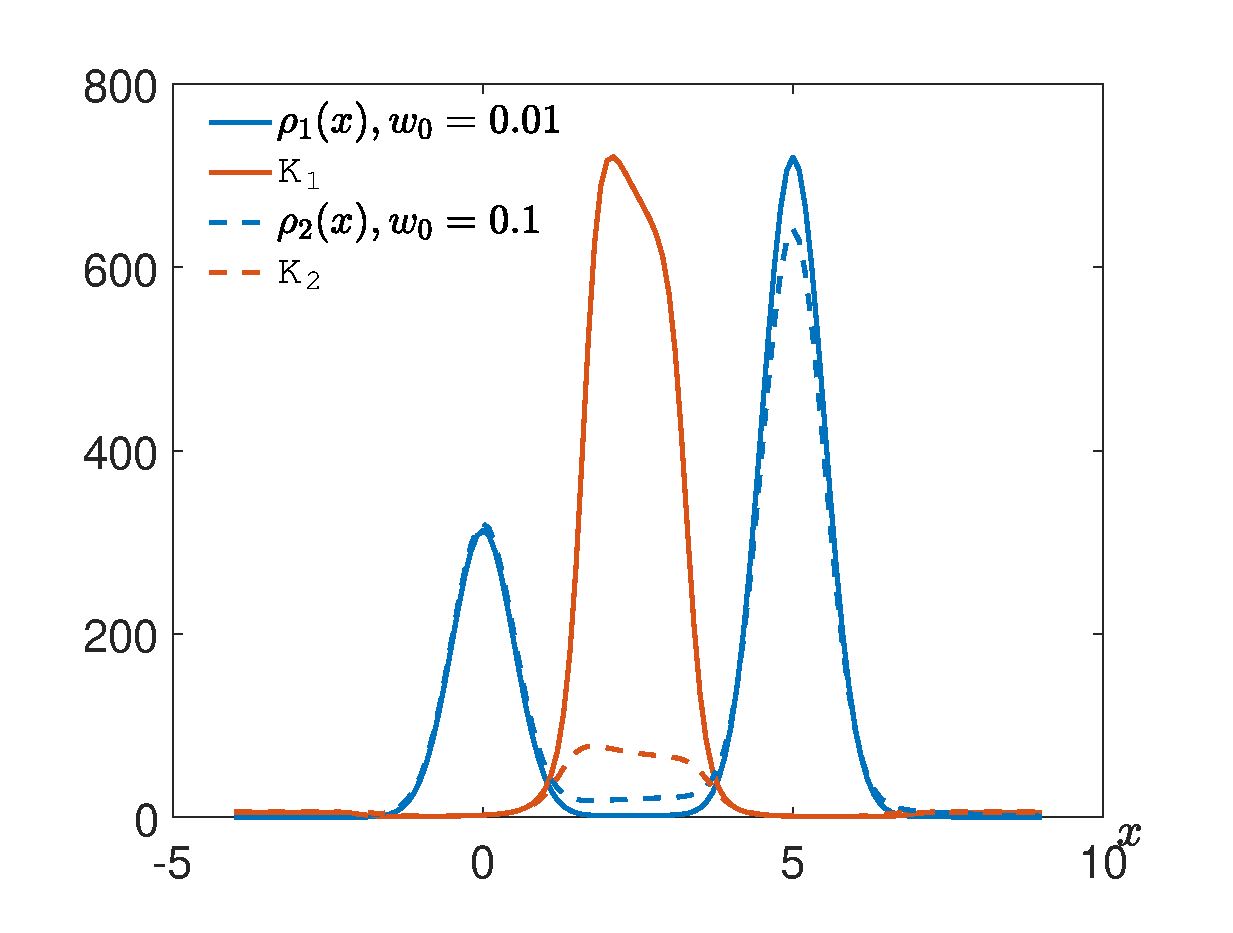
\includegraphics[width = 4in]{images/Chap4_Fig_gain_comparison}
	\caption{True FPF gains $\kFPF_1$ for $\pr_1$ with $w_{0}=0.01$ and $\kFPF_2$ for $\pr_2$ with $w_{0}=0.1$.}
	\label{fig:fpf_gain_num_issues}
\end{figure}

These numerical issues also impact the performance of $\gradTD$ learning algorithm. The rate of convergence of the parameters depends on properties of the stochastic process $\bfPhi$ described by Langevin's diffusion \eqref{e:diff_td_langevin_cts}, and the associated stochastic process that defines the eligibility vectors in \eqref{e:diff_td_gradTD_eligib}.  While a stationary version of this process exists in all of the examples considered here, it will be seen that in some examples the sample paths take on large values, which contributes to high variance.
These issues are most pronounced when the mixture density has a very shallow ``valley'', which is precisely the situation that leads to very large values of the true gain $\kFPF$. 

One of the practical approaches to prevent $\kFPF$ from taking extremely high values is to introduce a third Gaussian density $\pr_0$ to ``fill the well''. The third density $\pr_0(x)$ is chosen as $\mathcal{N}(\mu_{0}, \sigma_{0}^{2})$, where $\mu_0$ and $\sigma_0$ correspond to the sample mean and standard deviation of the entire particle population. The mixture probability $w_0$ of $\pr_0$ in the overall distribution $\pr$ is forced to be greater than a threshold value. This is further illustrated by the sharp decline in the peak magnitude of $\kFPF_1$ compared to $\kFPF_2$ in \Fig{fig:fpf_gain_num_issues}.

\subsection{Gain function approximation for a fixed $t$}
In each of the following experiments the density $\pr\in\clP$ was chosen with $m=2$,
\begin{equation}
\pr = 0.5 \mathcal{N}(-1, 0.4472) + 0.5 \mathcal{N}(1, 0.4472),
\label{e:fpf_gaussian_mixture_example}
\end{equation}
such that each component has a variance of $0.2$. The observation function is linear, with $c(x)\equiv x$ and $\sigma_W = 1$. 

\subsection*{Linear parameterization}
\label{s:linear_param}
It is reasonable to search for a basis that offers flexibility in regions where the density $\pr$ takes on non-negligible values. We consider three different choices for basis functions as follows:
\begin{romannum}
\item A polynomial basis, such that $\basis_n(x) = x^n$ for $1 \leq n \leq \ell$.
\item A Fourier basis composed of sines and cosines of harmonic frequencies, $\basis_n(x) = \sin(n x), \basis_{n+1}(x) = \cos(n x)$ for $1 \leq n \leq \ell/2$.
\item Polynomials weighted by the component densities $\pr_i$, defined as: 
\begin{equation}
\{\basis_n(x) : x\in\Re,\ 1\le n\le \ell\}  = \{ x^k \pr_i(x) :  1\le k \le \ell/2, \,  i=1,2\}
\label{e:wt_polynomial_basis}
\end{equation}
\end{romannum}
It is not difficult to show that the true gain is nearly constant for large $x$, with $\lim_{|x|\to\infty} \kFPF(x) = \Kkal$. The limit corresponds to the Kalman-like gain $\Kkal$ obtained for the model in which $\pr$ is replaced by $\pr_i$  (the Gaussian density with the highest variance). The function $\basis_n(x) = x$ is added to the basis (for choices ii and iii, it is already included in i), such that $\nabla \basis(x)\equiv 1$ is present to account for this constant asymptotic gain value. The class $\clK$ is defined using this basis:
\begin{equation*}
K_\param = \param^{\transpose}\gradbasis = \sum_{n=1}^{\ell}\param_{n}\gradbasis_{n}\,, \quad\param\in\Re^{\ell}
\end{equation*}

\subsection*{Nonlinear parameterization}
\label{s:nl_param}
In a nonlinear parameterization setting, the following form is chosen for the class $\clK$.
\begin{equation*}
K_\param(x) = K_{0} + \sum_{i=1}^{l} \xi_{i}^{\param}(x)
\end{equation*}
Of the various nonlinear parameterizations tested, the following produced the best results,
\begin{equation*}
\xi_{i}^{\param}(x) = \dfrac{a_{i}}{(x -b_{i})^2 + c_{i}^2}
\end{equation*}
The coefficients $\alpha_i  = \{a_i, b_i, c_i \}, K_0$ constitute the parameters to be estimated.
In the simulation results surveyed here  $l=3$ and hence, $\param \in \Re^{\ell}$ with $\ell=10$.
%\begin{figure}[htbp]
%	\Ebox{0.9}{images/Chap4_Fig_nltdB}
%	\caption{Performance of nonlinear parameterization $\nabla$-LSTD}
%	\label{f:nltd}
%\end{figure}

Optimal nonlinear parameterization can be obtained by running $\nabla$-TD learning using stochastic approximation techniques, discussed in \Section{s:diff_td_nl_param}. Two such techniques were used, namely stochastic Newton Raphson and approximation with Polyak averaging \cite{bor08a}. The scalar gain term $\gamma_t$ is set to $1/(t+1)^{\beta}$. For stochastic Newton Raphson, $\beta$ is chosen to be $1$, and $\beta=0.6$ was chosen for Polyak averaging.

\subsection*{Basis-free algorithms}
The following basis-free approximation approaches were compared:
\begin{romannum}
\item RKHS based methods, both optimal and simplified versions of \Section{s:rkhs}.
\item RKHS method with optimal mean, using the constant gain approximation (RKHS-OM) of \Section{s:rkhs_om}.
\item Markov semigroup approximation method of \Section{s:coifman}.
\end{romannum}
\begin{figure}[htbp]
	\centering
	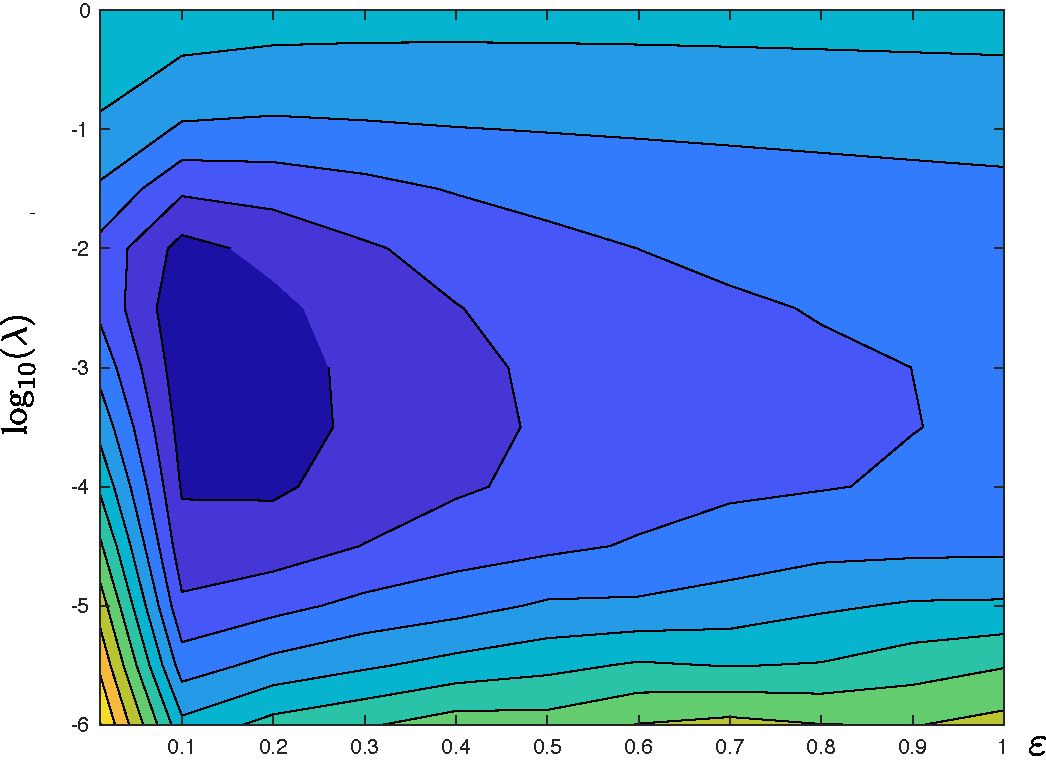
\includegraphics[width = 4in]{images/Chap4_log_mse_contour_2m}
	\caption{Contour plots of average over $100$ trials of $\log(\|\kFPF - \widehat{\kFPF}\|^2_{L^2})$ with $\lambda$ and $\epsy$ with $N=500$.}
	\label{fig:log_mse_contour}
\end{figure}
 For each of the RKHS methods, the standard Gaussian kernel \eqref{e:rkhs_gaussian_kernel} was used, centered at the particle locations $\{x^i\}_1^N$. \Fig{fig:log_mse_contour} illustrates the sensitivity in gain approximation to the hyperparameters $\lambda$ and $\epsy$ for $N=500$. The contour plots in \Fig{fig:log_mse_contour} correspond to the log of the average mean square error in the gain approximation $\|\kFPF - \widehat{\kFPF} \|^2_{L^2}$; estimated by observations over $100$ independent trials. It is evident that a larger value for $\lambda$ prevents overfitting and a smaller value for $\epsy$ provides more flexibility. With increase in $N$, the best choices of $\lambda$ and $\epsy$ show a declining trend. Based on these results from sensitivity analysis, $\lambda = 10^{-2}$ and $\epsy = 0.1$ was chosen for the RKHS methods.

\subsection*{Results and discussion}
\begin{figure}[htbp]
	\centering
	\mbox{
		\subfigure [] {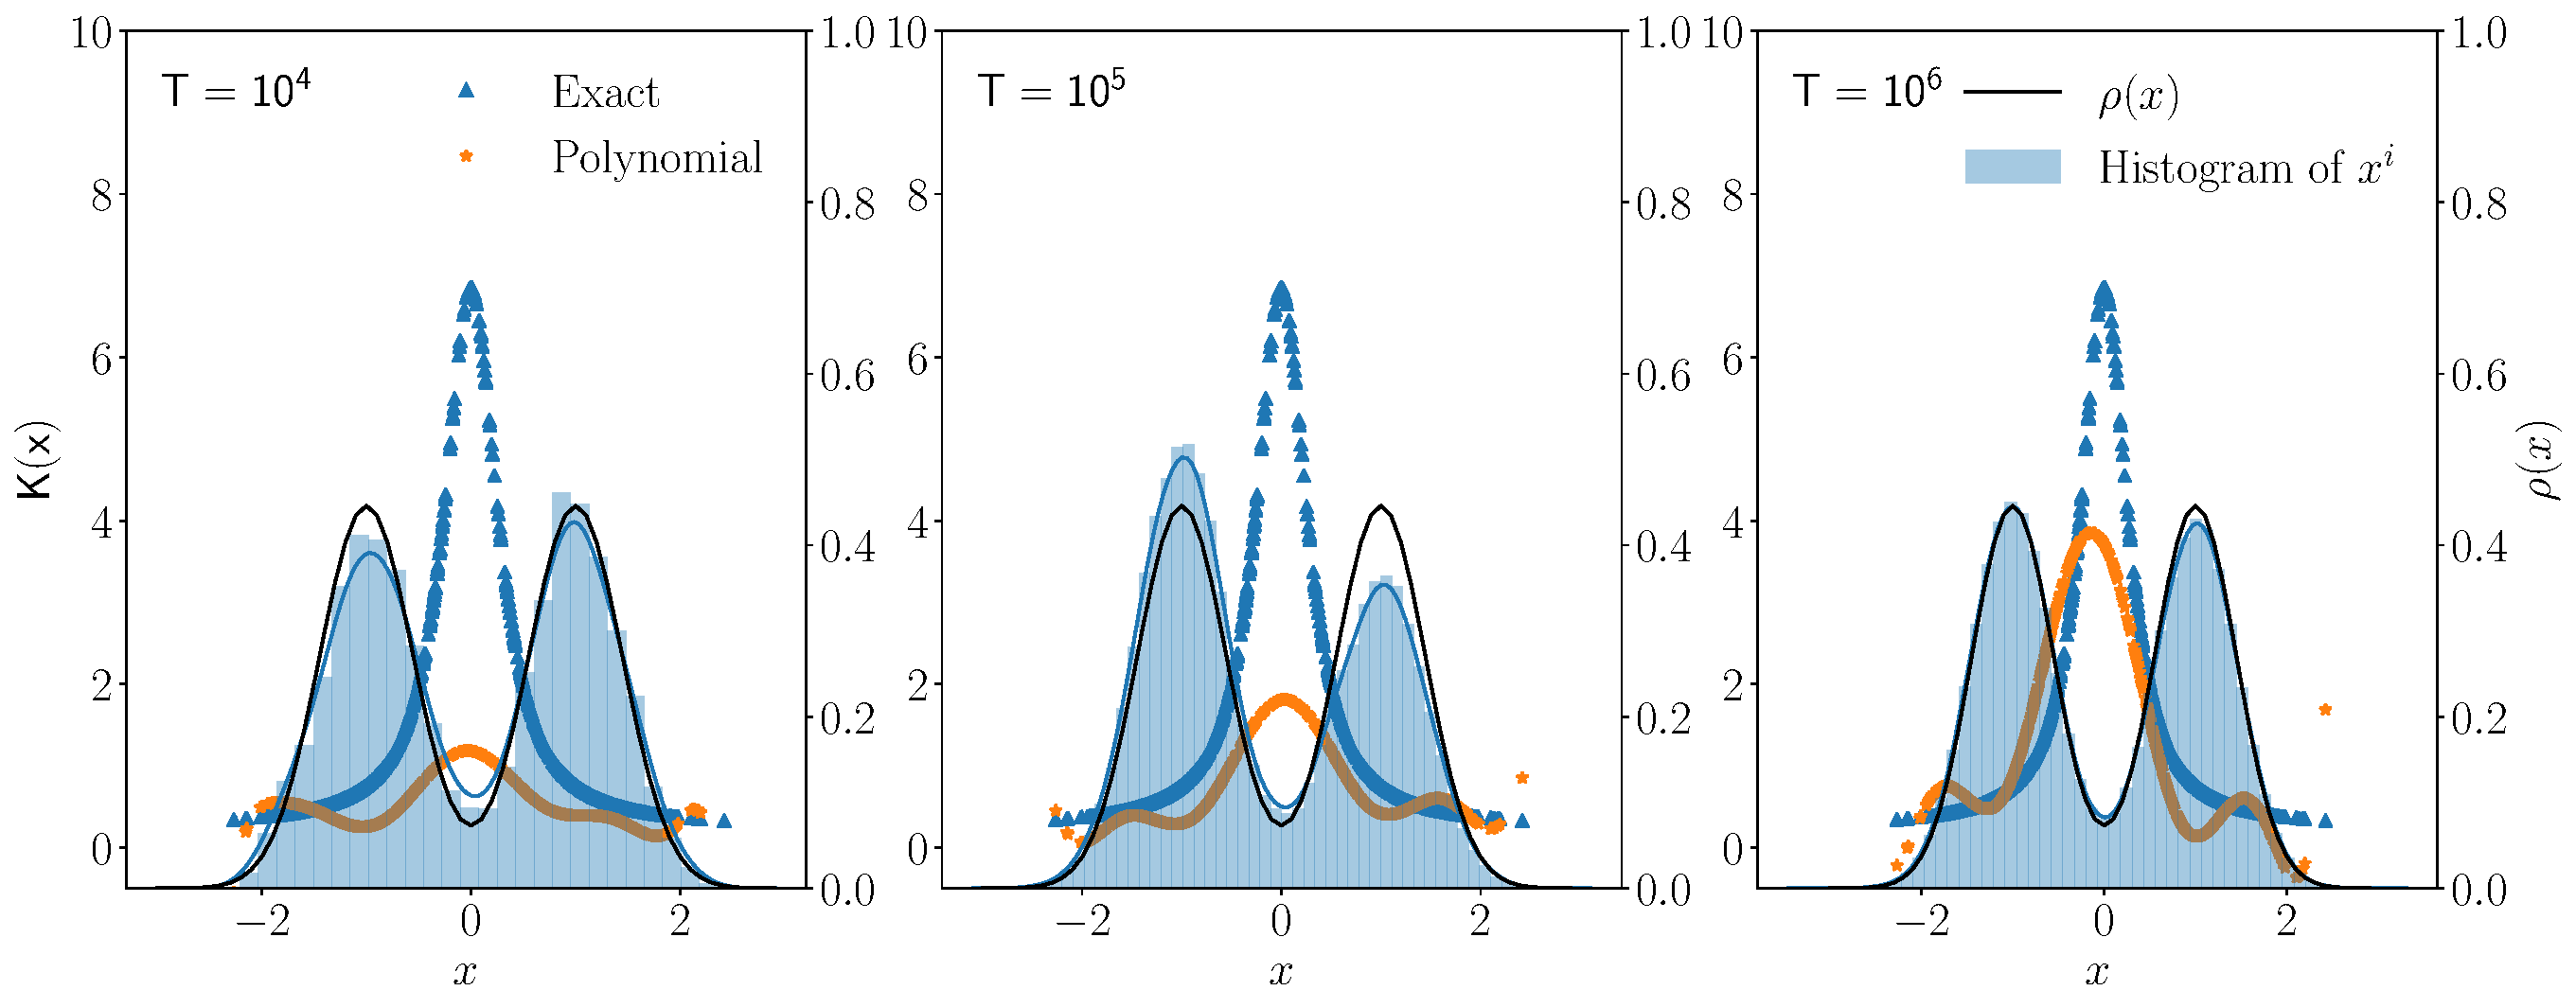
\includegraphics[width=6in]{images/Chap4_diff_td_linear_polynomials}} 
	}
	\mbox{
		\subfigure [] {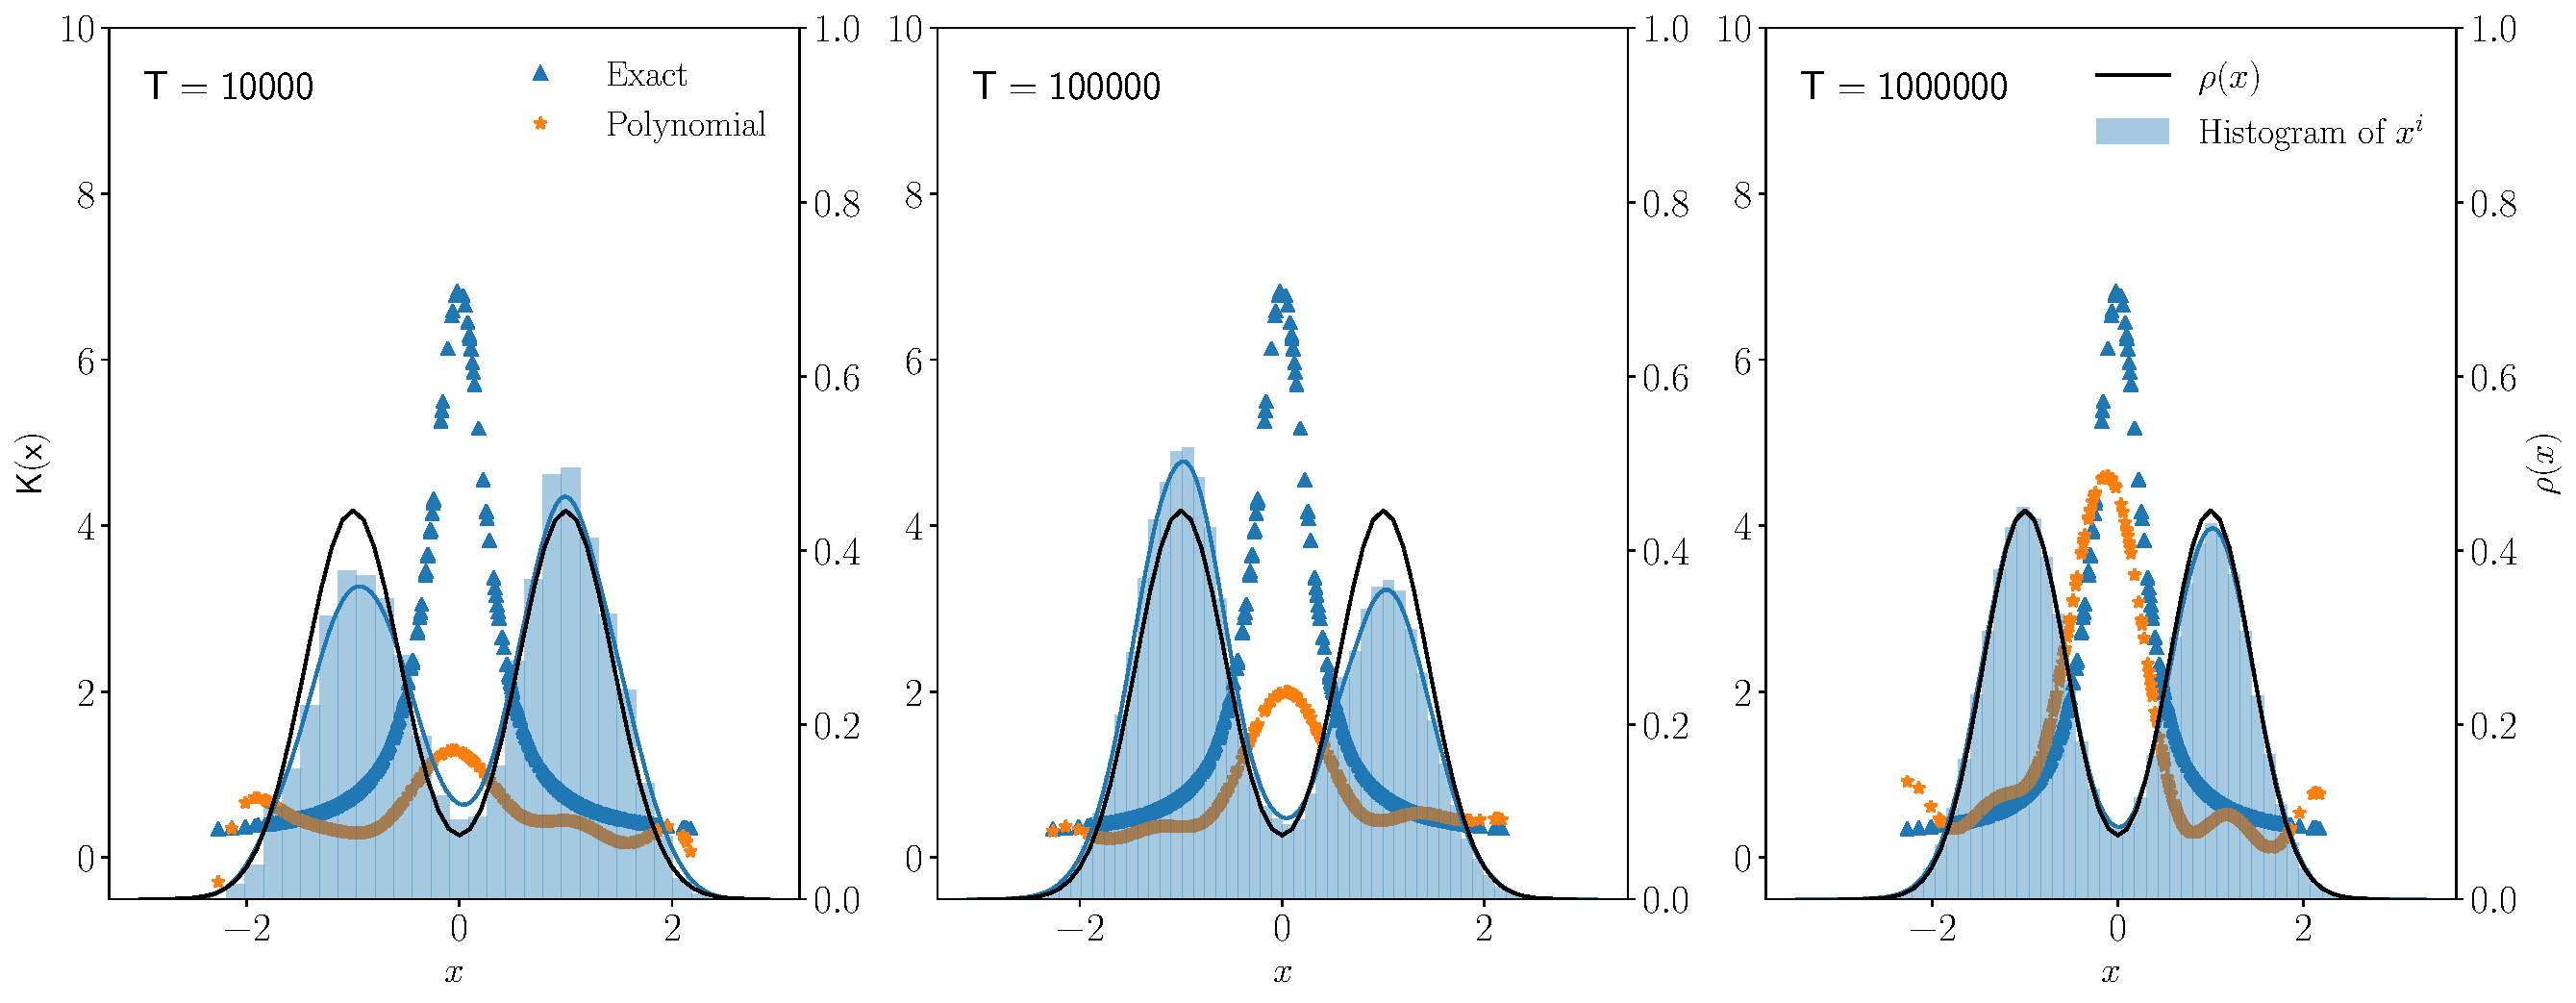
\includegraphics[width=6in]{images/Chap4_diff_td_linear_fourier}} 
	}
	\mbox{
		\subfigure [] {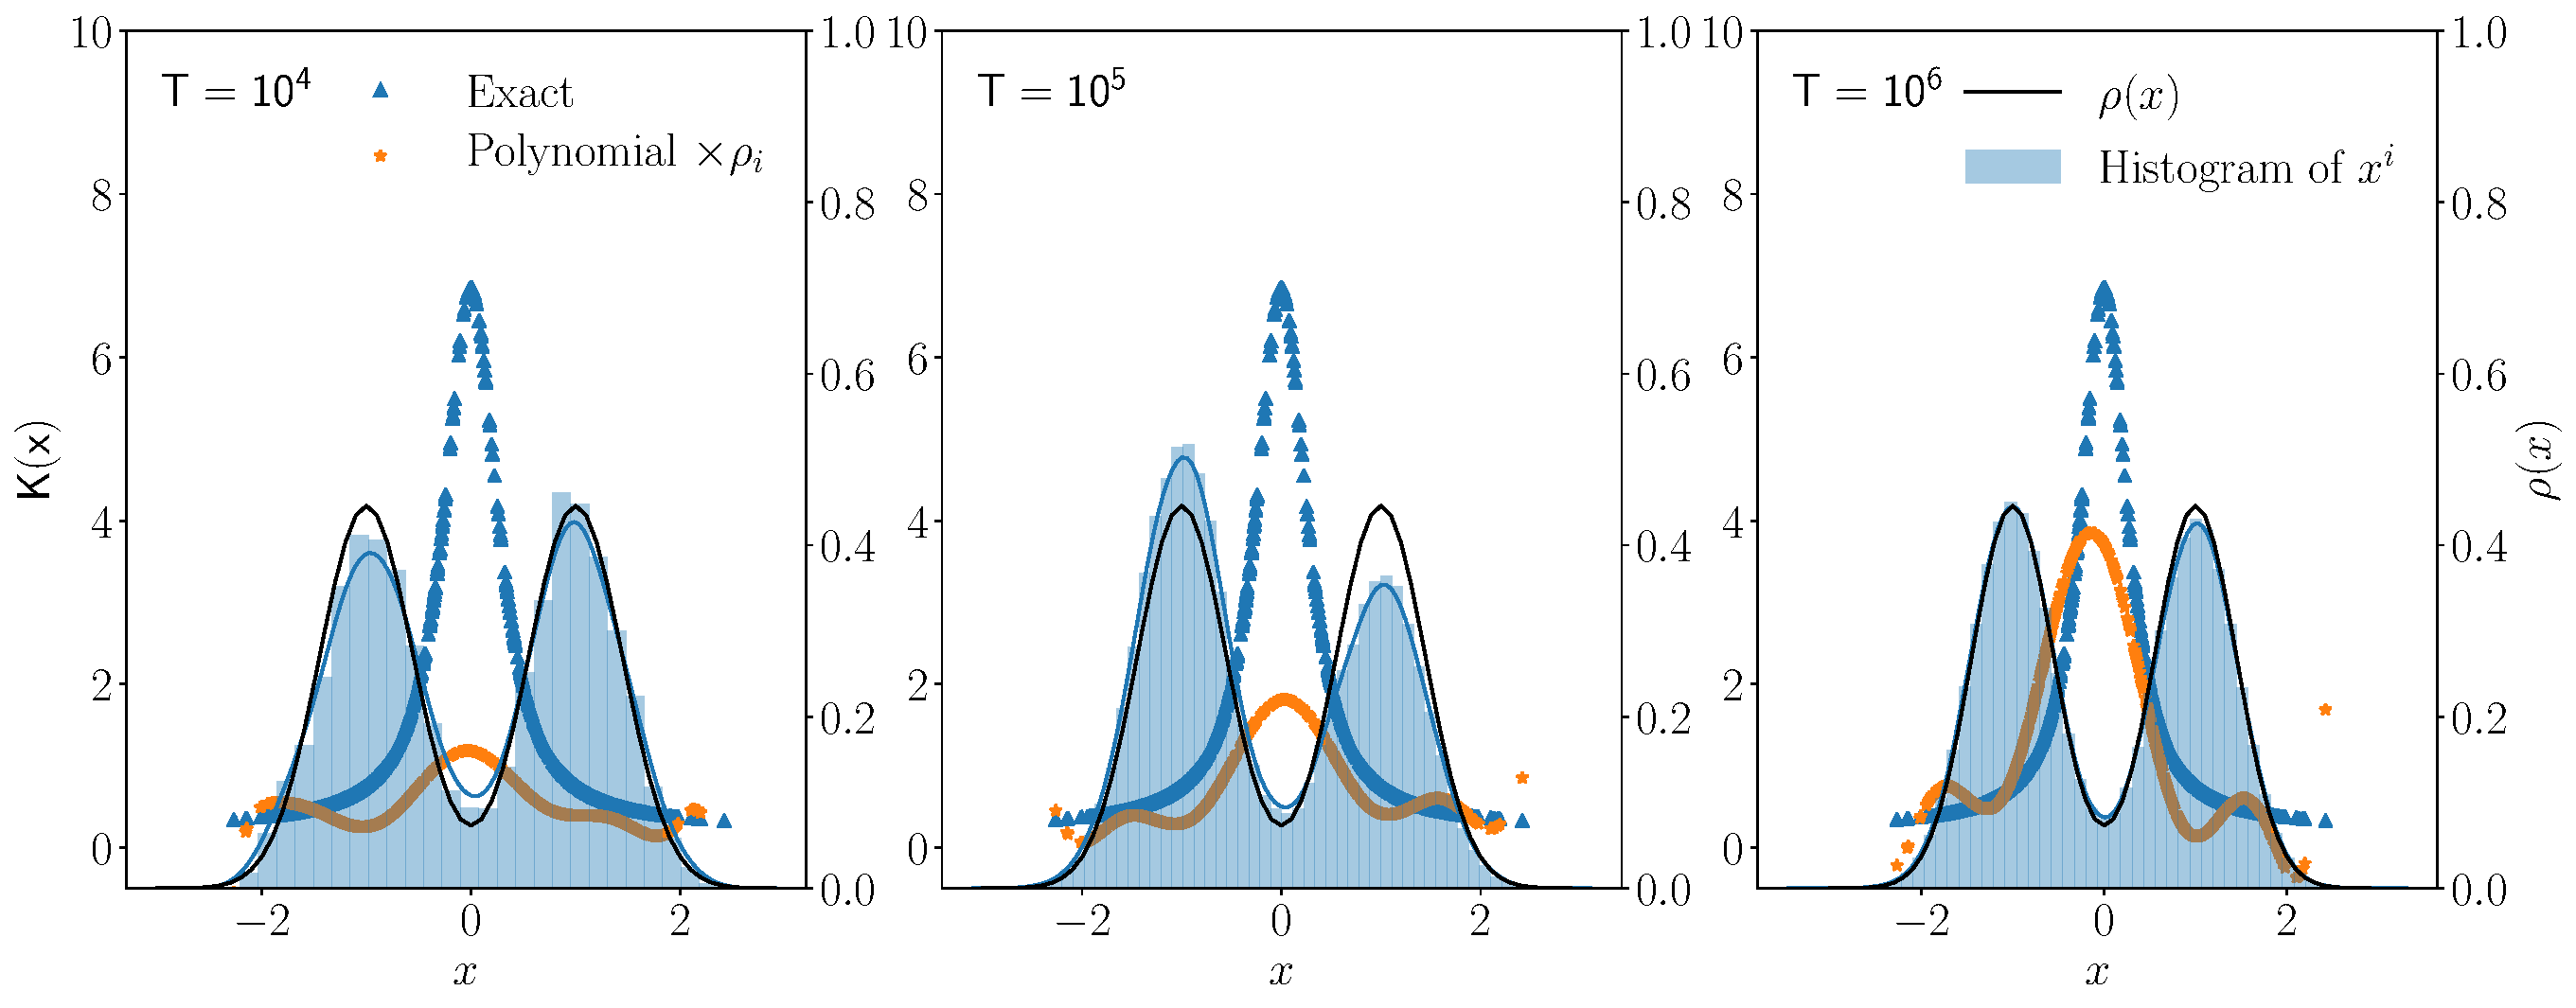
\includegraphics[width = 6in]{images/Chap4_diff_td_linear_wt_polynomials}} 
	}
	\caption[LSTD performance]{Gain function approximations using $\gradTD$ learning algorithm (\Section{s:diff_td_learning}) using a linear parameterization \cite{raddevmey16} A) Polynomial basis, B) Fourier basis consisting of sines and cosine functions, C) Polynomials weighted by $\pr_i$.}
	\label{fig:diff_td_linear}
\end{figure}

\begin{figure}
	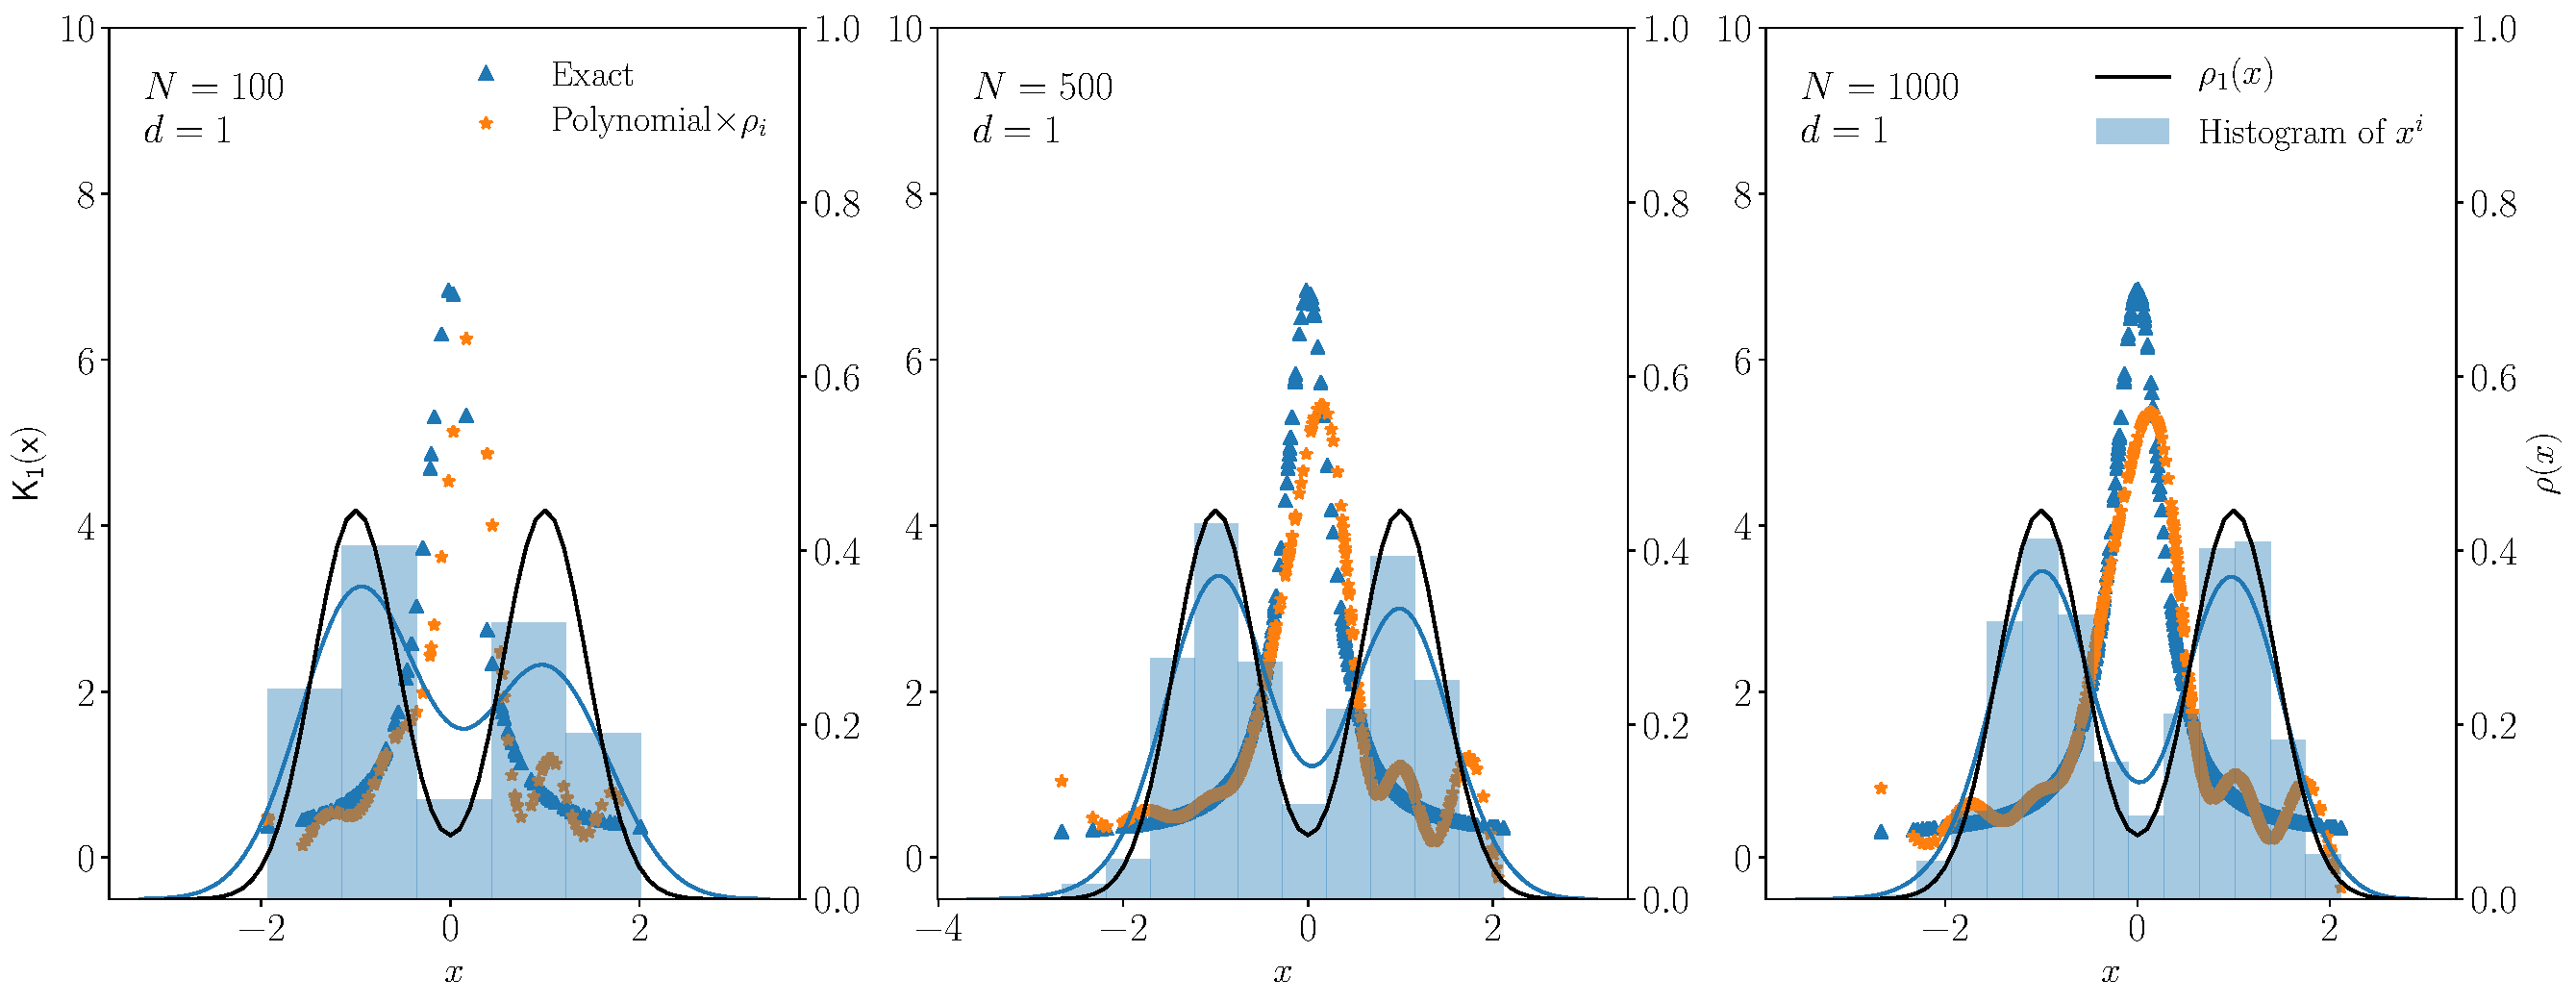
\includegraphics[width=6in]{images/Chap4_lang_td_wt_polynomials}
	\caption[Finite dimensional polynomial basis]{Gain function approximations using a $10$-dimensional polynomial$\times \pr_i$ basis using $\gradTD$ learning for Langevin diffusion (\Section{s:diff_td_langevin})}
	\label{fig:diff_td_lang_linear}
\end{figure}

\begin{figure}[htbp]
	\centering
	\mbox{
		\subfigure [] {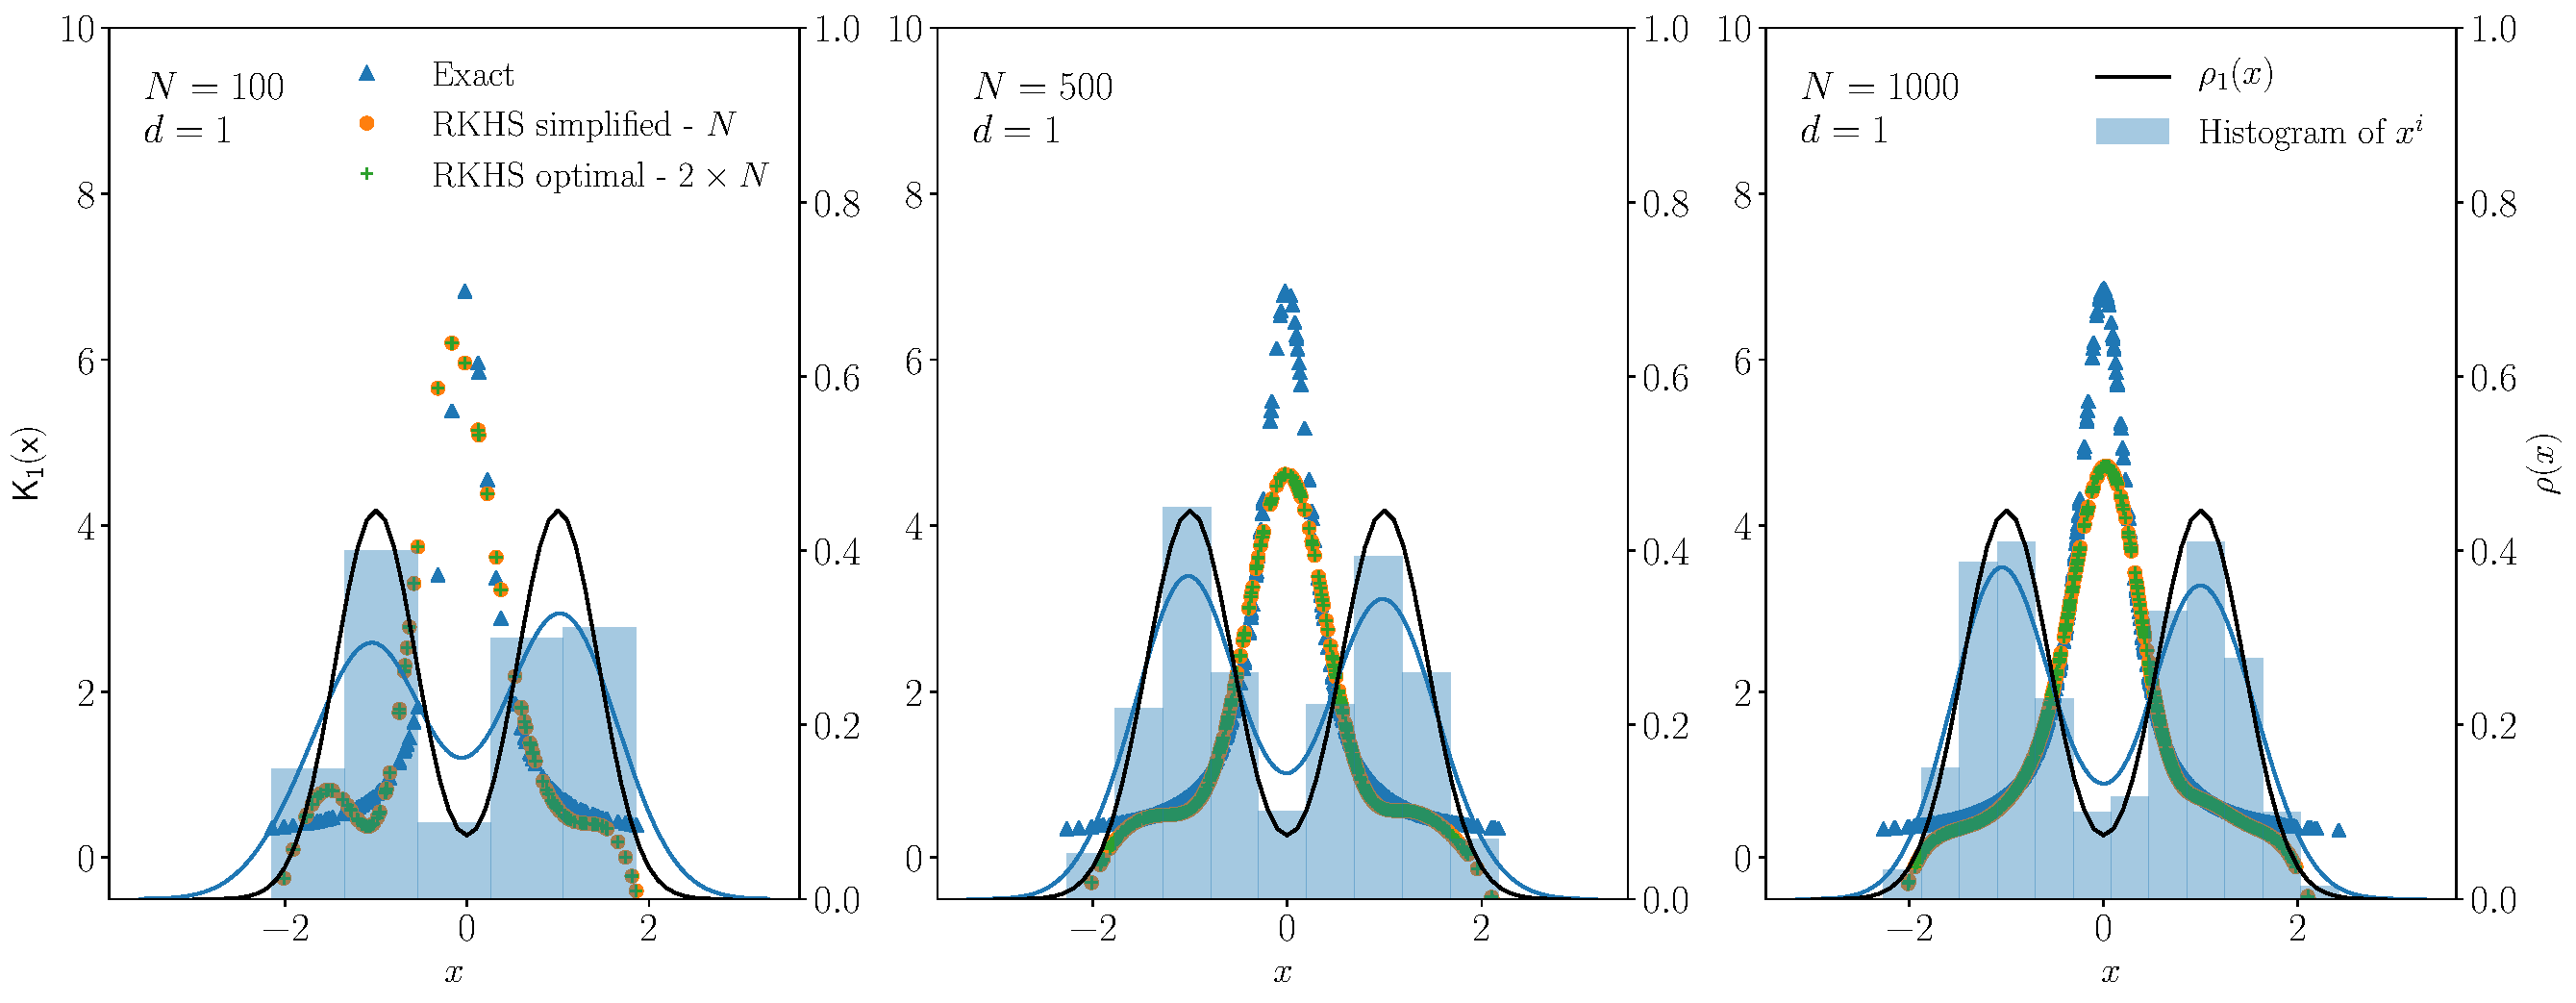
\includegraphics[width=6in]{images/Chap4_N_dN}} 
		\label{fig:A}
	}
	\mbox{
		\subfigure [] {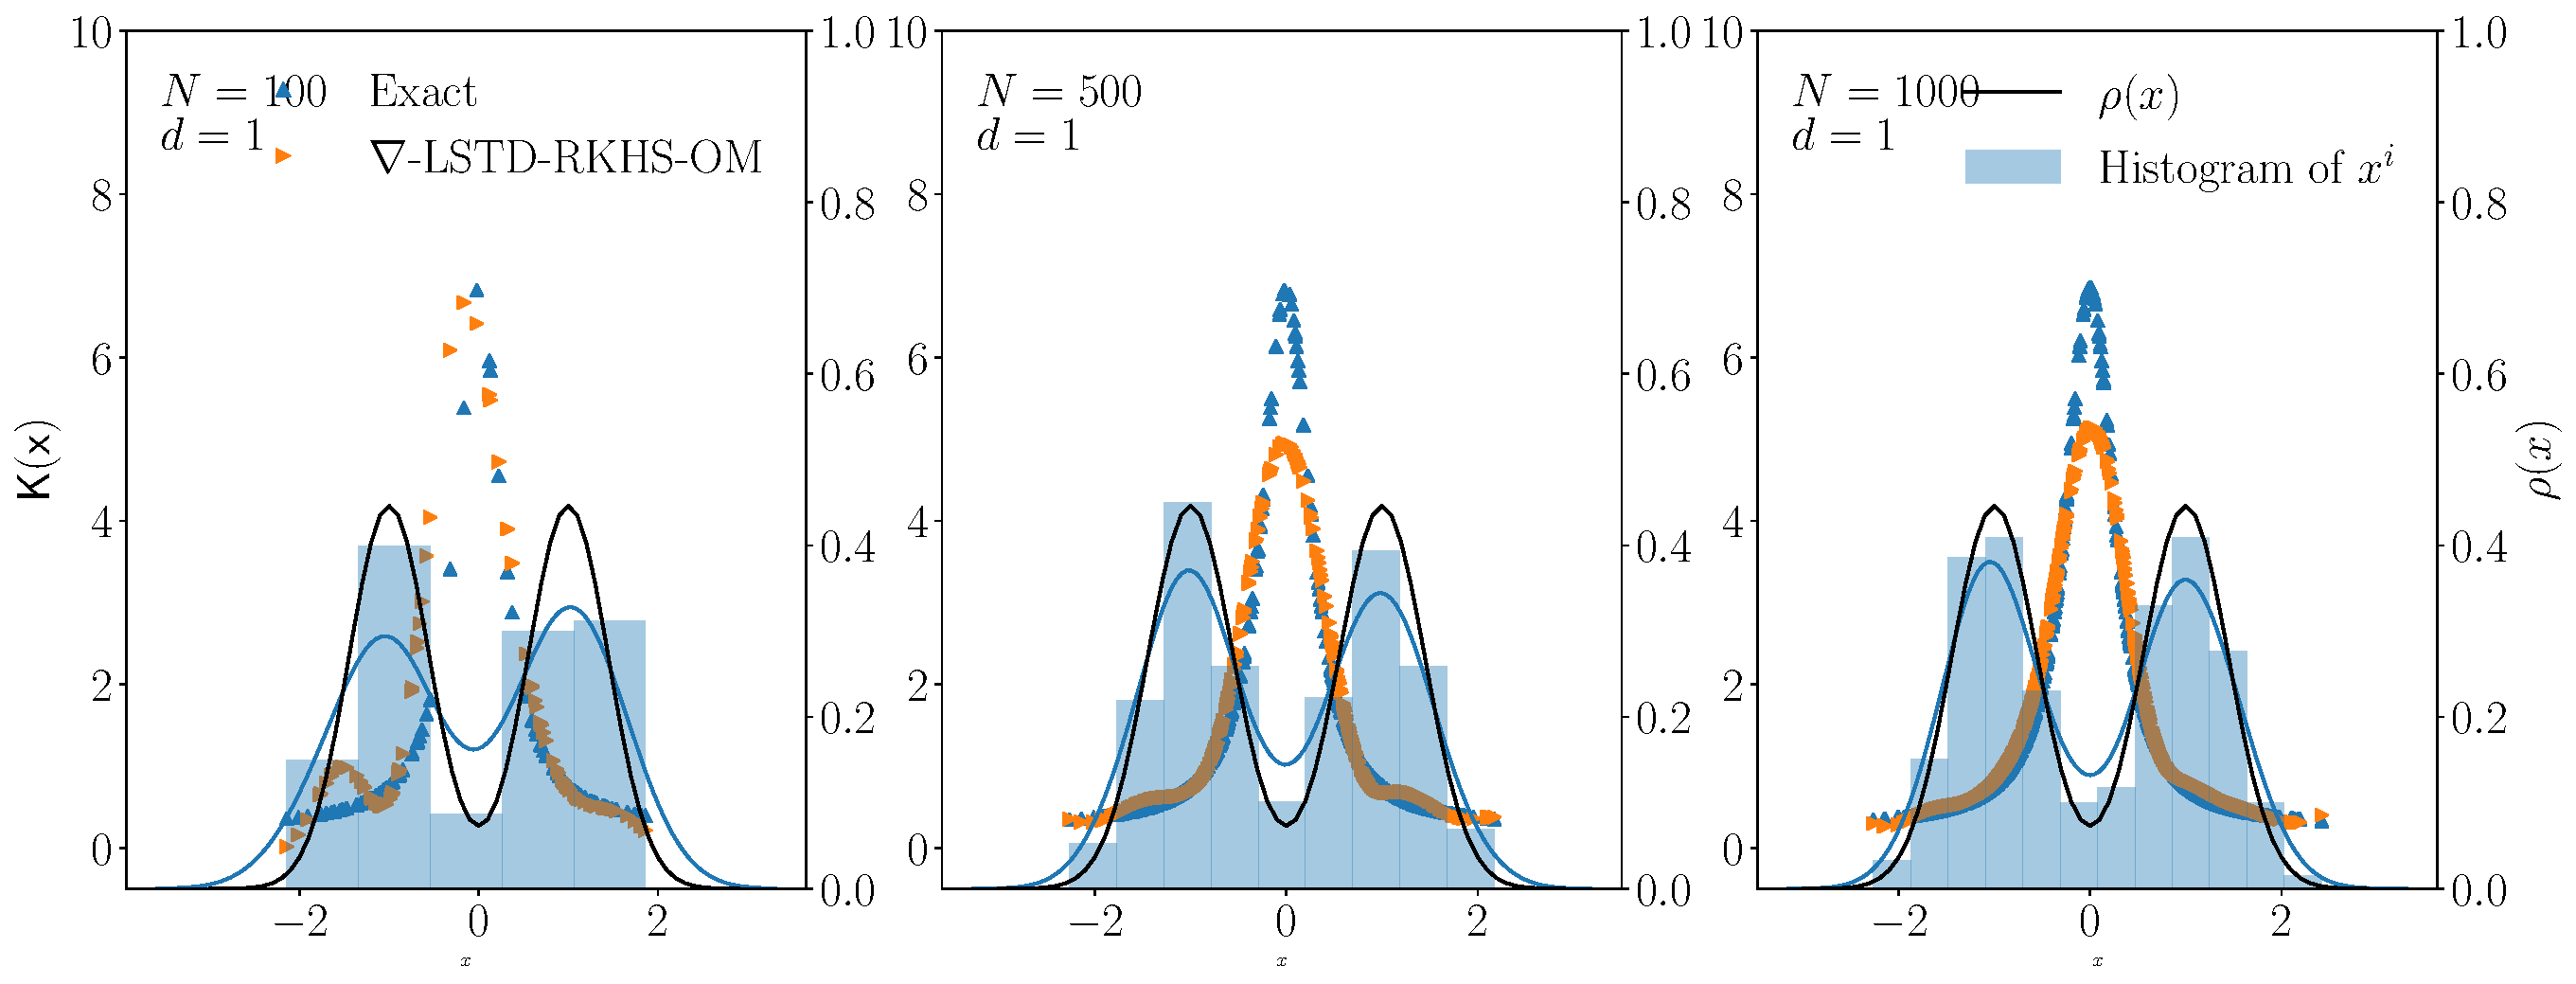
\includegraphics[width=6in]{images/Chap4_rkhs_om}} 
	}
	\mbox{
		\subfigure [] {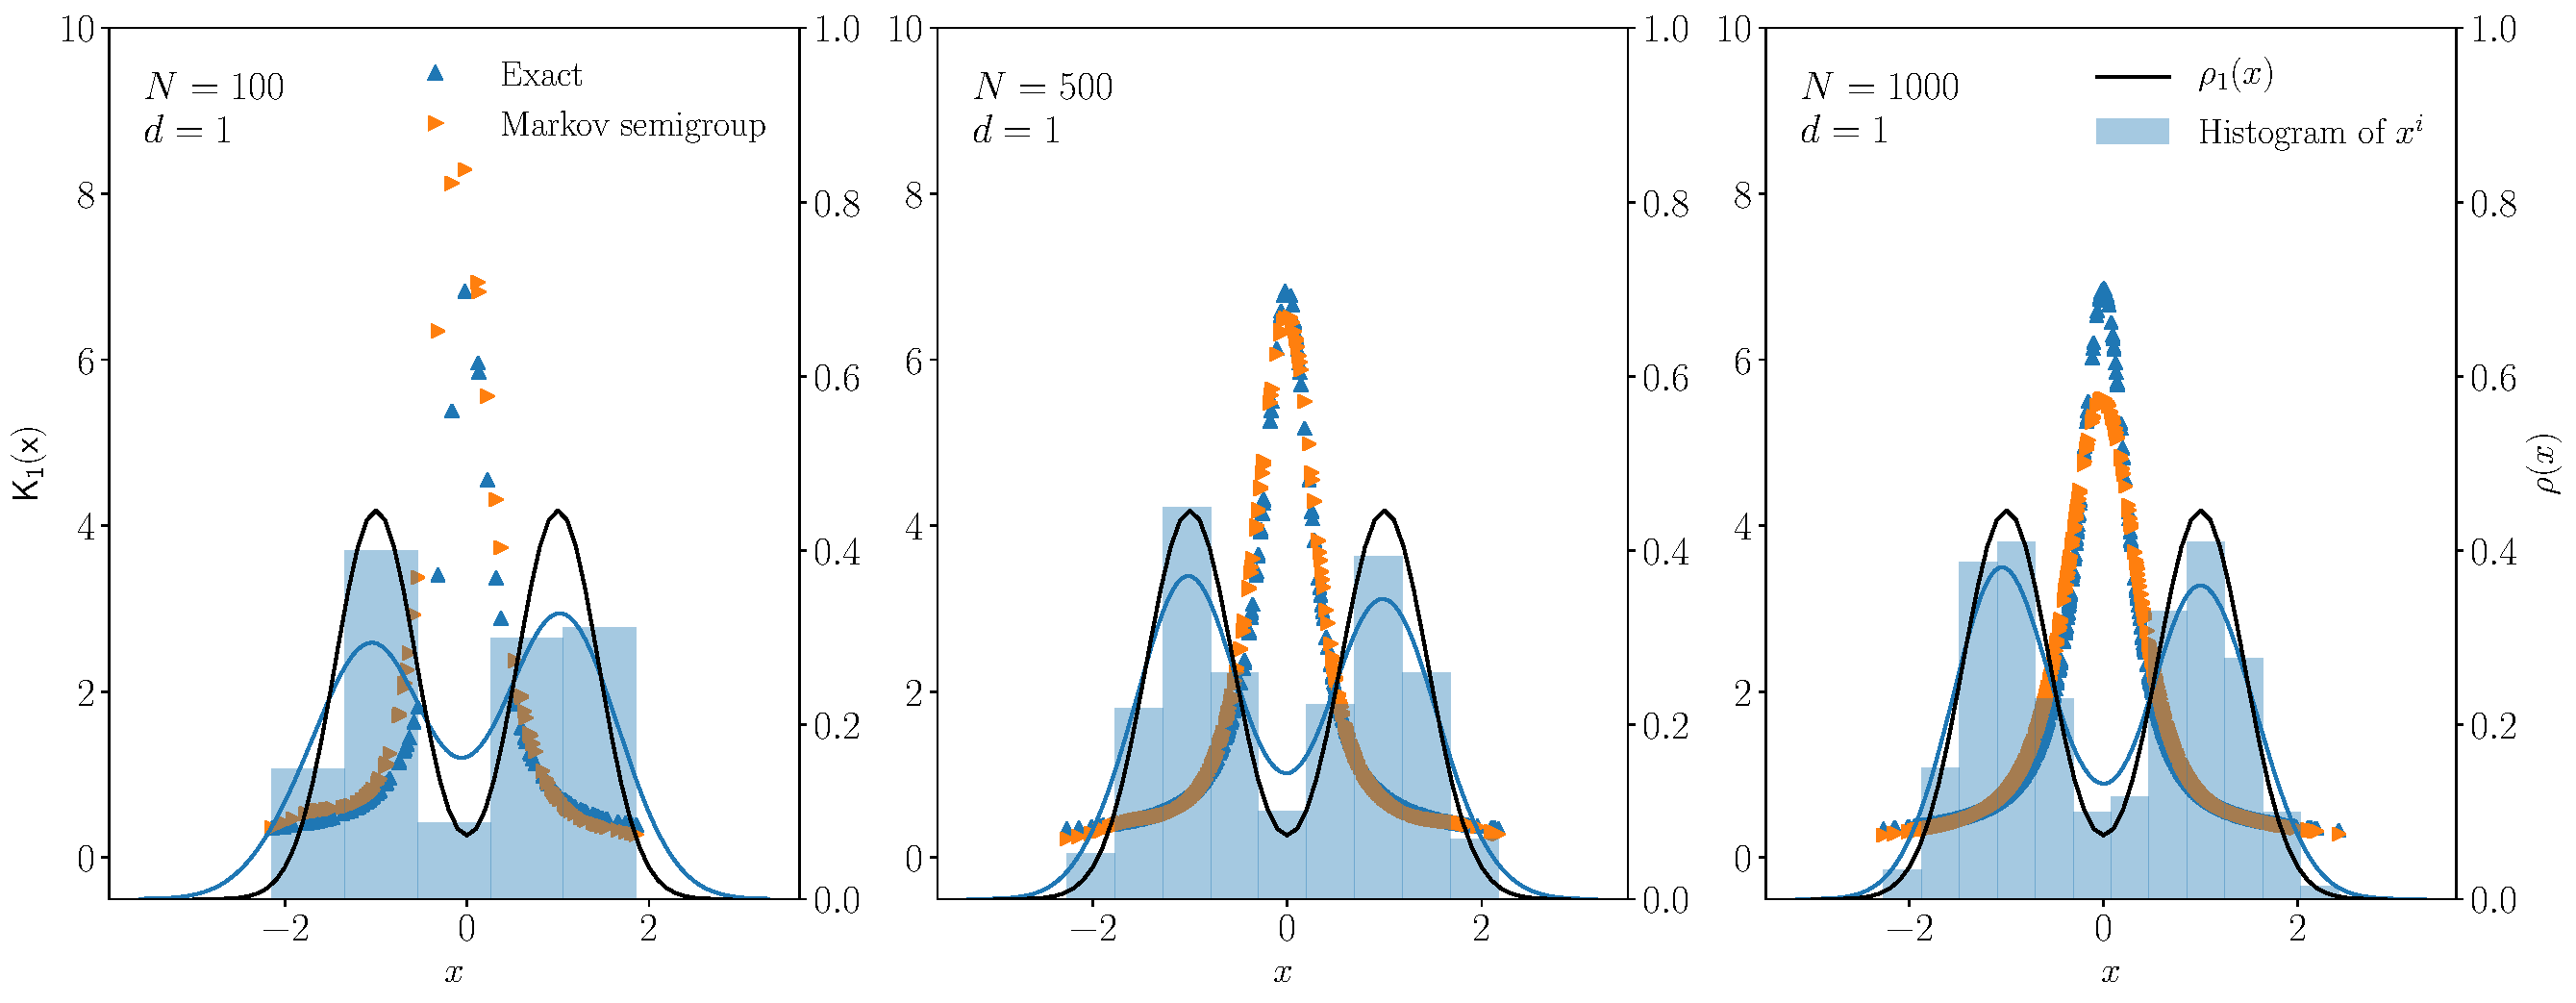
\includegraphics[width = 6in]{images/Chap4_coif}} 
	} 
	\caption[RKHS and coifman performance]{Gain function approximations using basis-free approaches - A) RKHS optimal and RKHS simplified with $2N$ and $N$ parameters respectively \cite{radmey18a}, B) RKHS-OM method \cite{radmey19}, C) Markov semigroup approximation \cite{tagmeh16}.}
	\label{fig:diff_td_rkhs_coif}
\end{figure}
 \anand{Change $\pr_1$ in the legend to $\pr$}
\begin{figure}
	\centering
	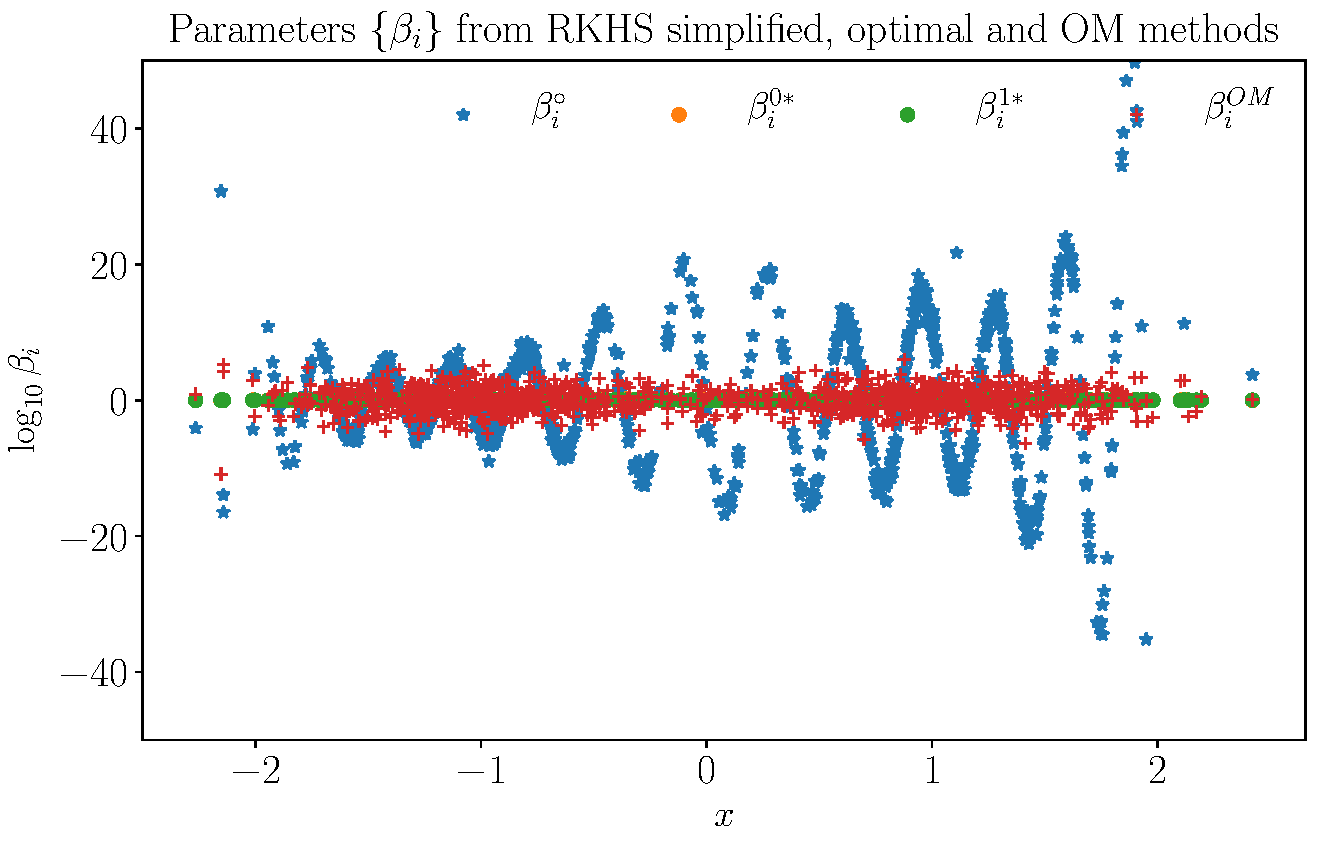
\includegraphics[width=5in]{images/Chap4_beta_comparison}
	\caption[RKHS and coifman performance]{Magnitudes of $\{\beta_i\}$ obtained from A) RKHS optimal, B) RKHS simplified and C) RKHS OM algorithms}
	\label{fig:beta_comparison}
\end{figure}

\begin{figure}
	\centering
	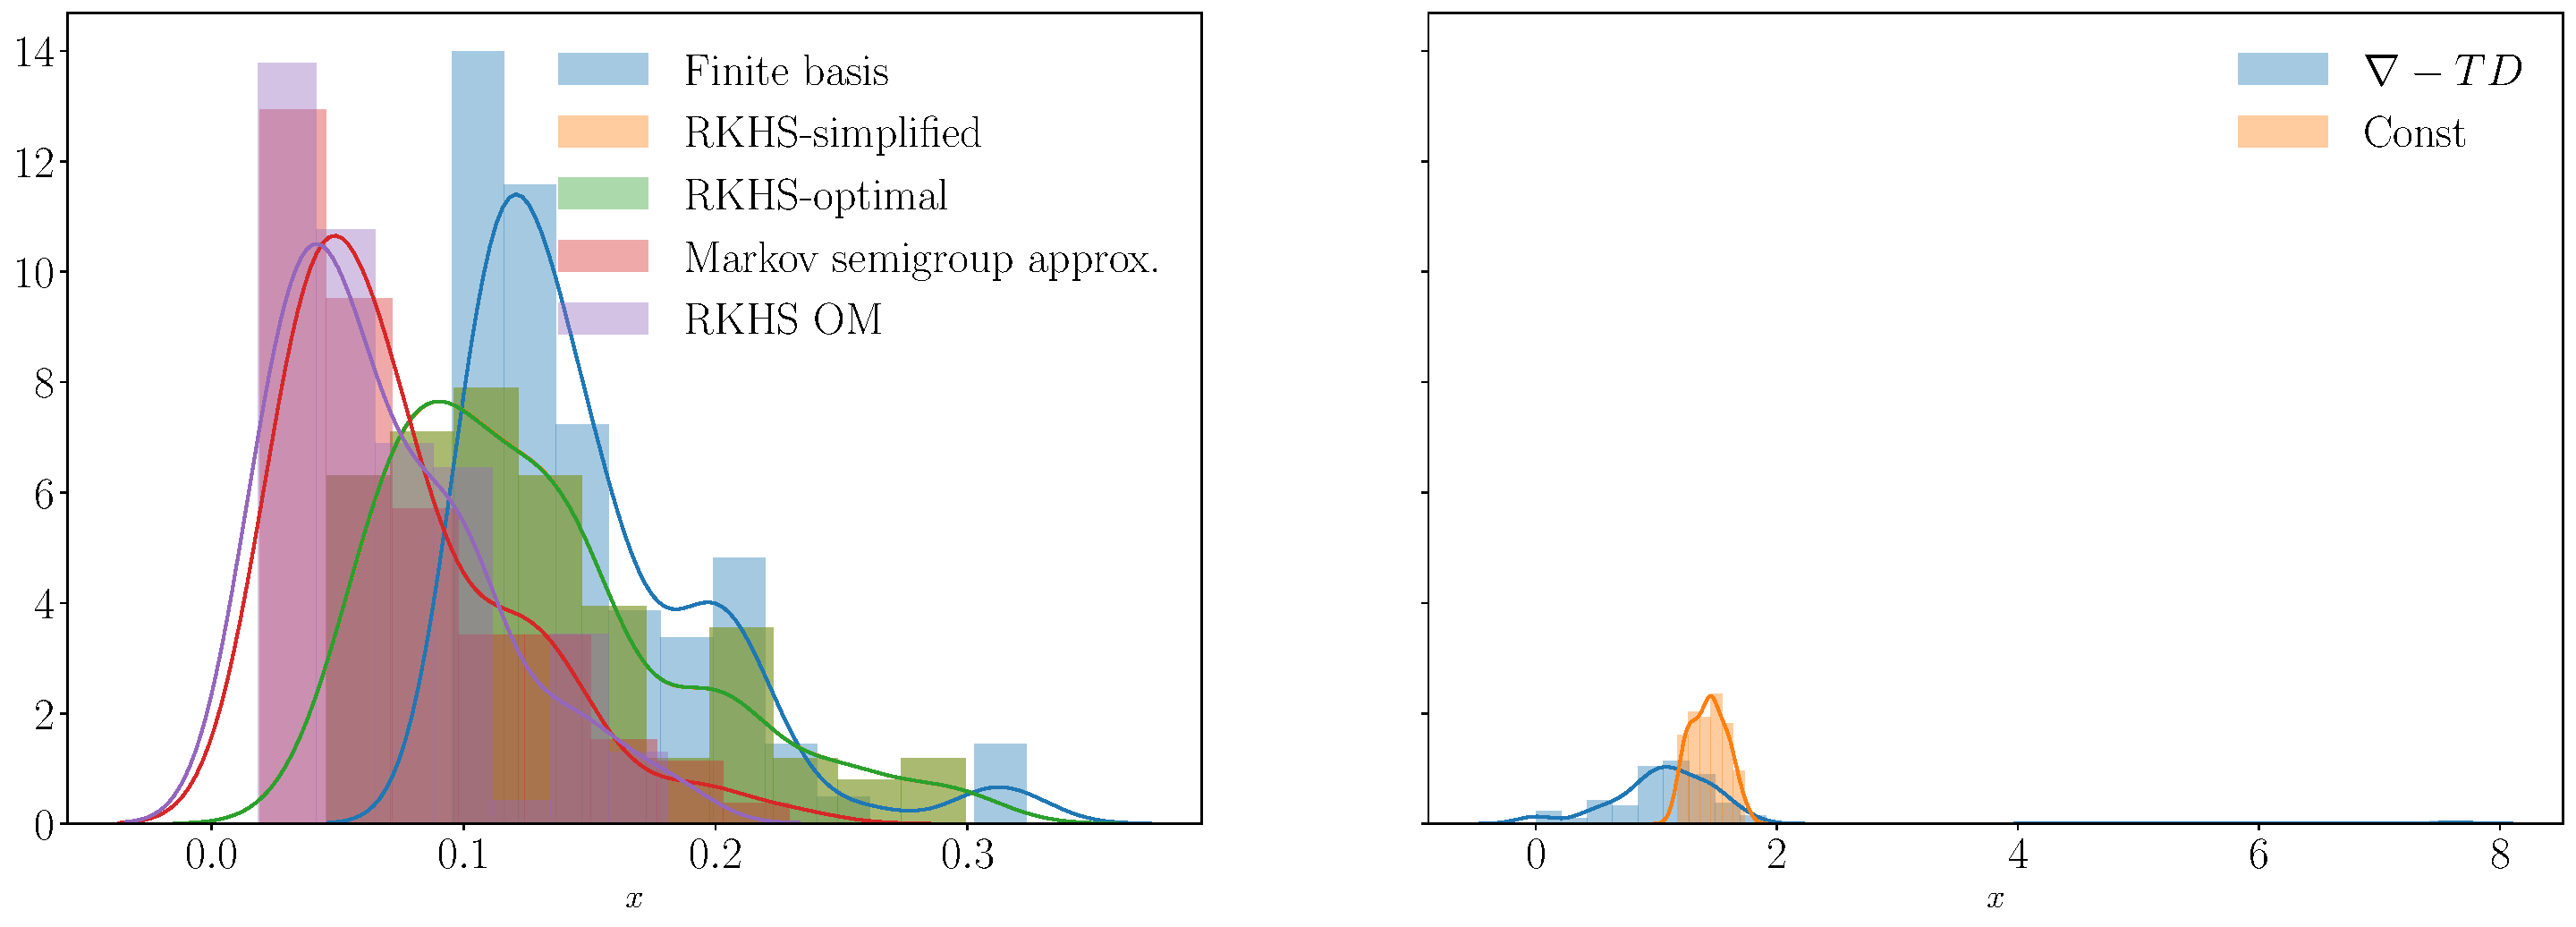
\includegraphics[width=6in]{images/Chap4_hist_mse_d1_runs100}
	\caption[RKHS and coifman performance]{Histograms of MSE obtained using various methods for $d=1,N=1000$ over $100$ independent trials.}
	\label{fig:hist_mse}
\end{figure}

\begin{figure}[htbp]
	\centering
	\mbox{
		\subfigure [] {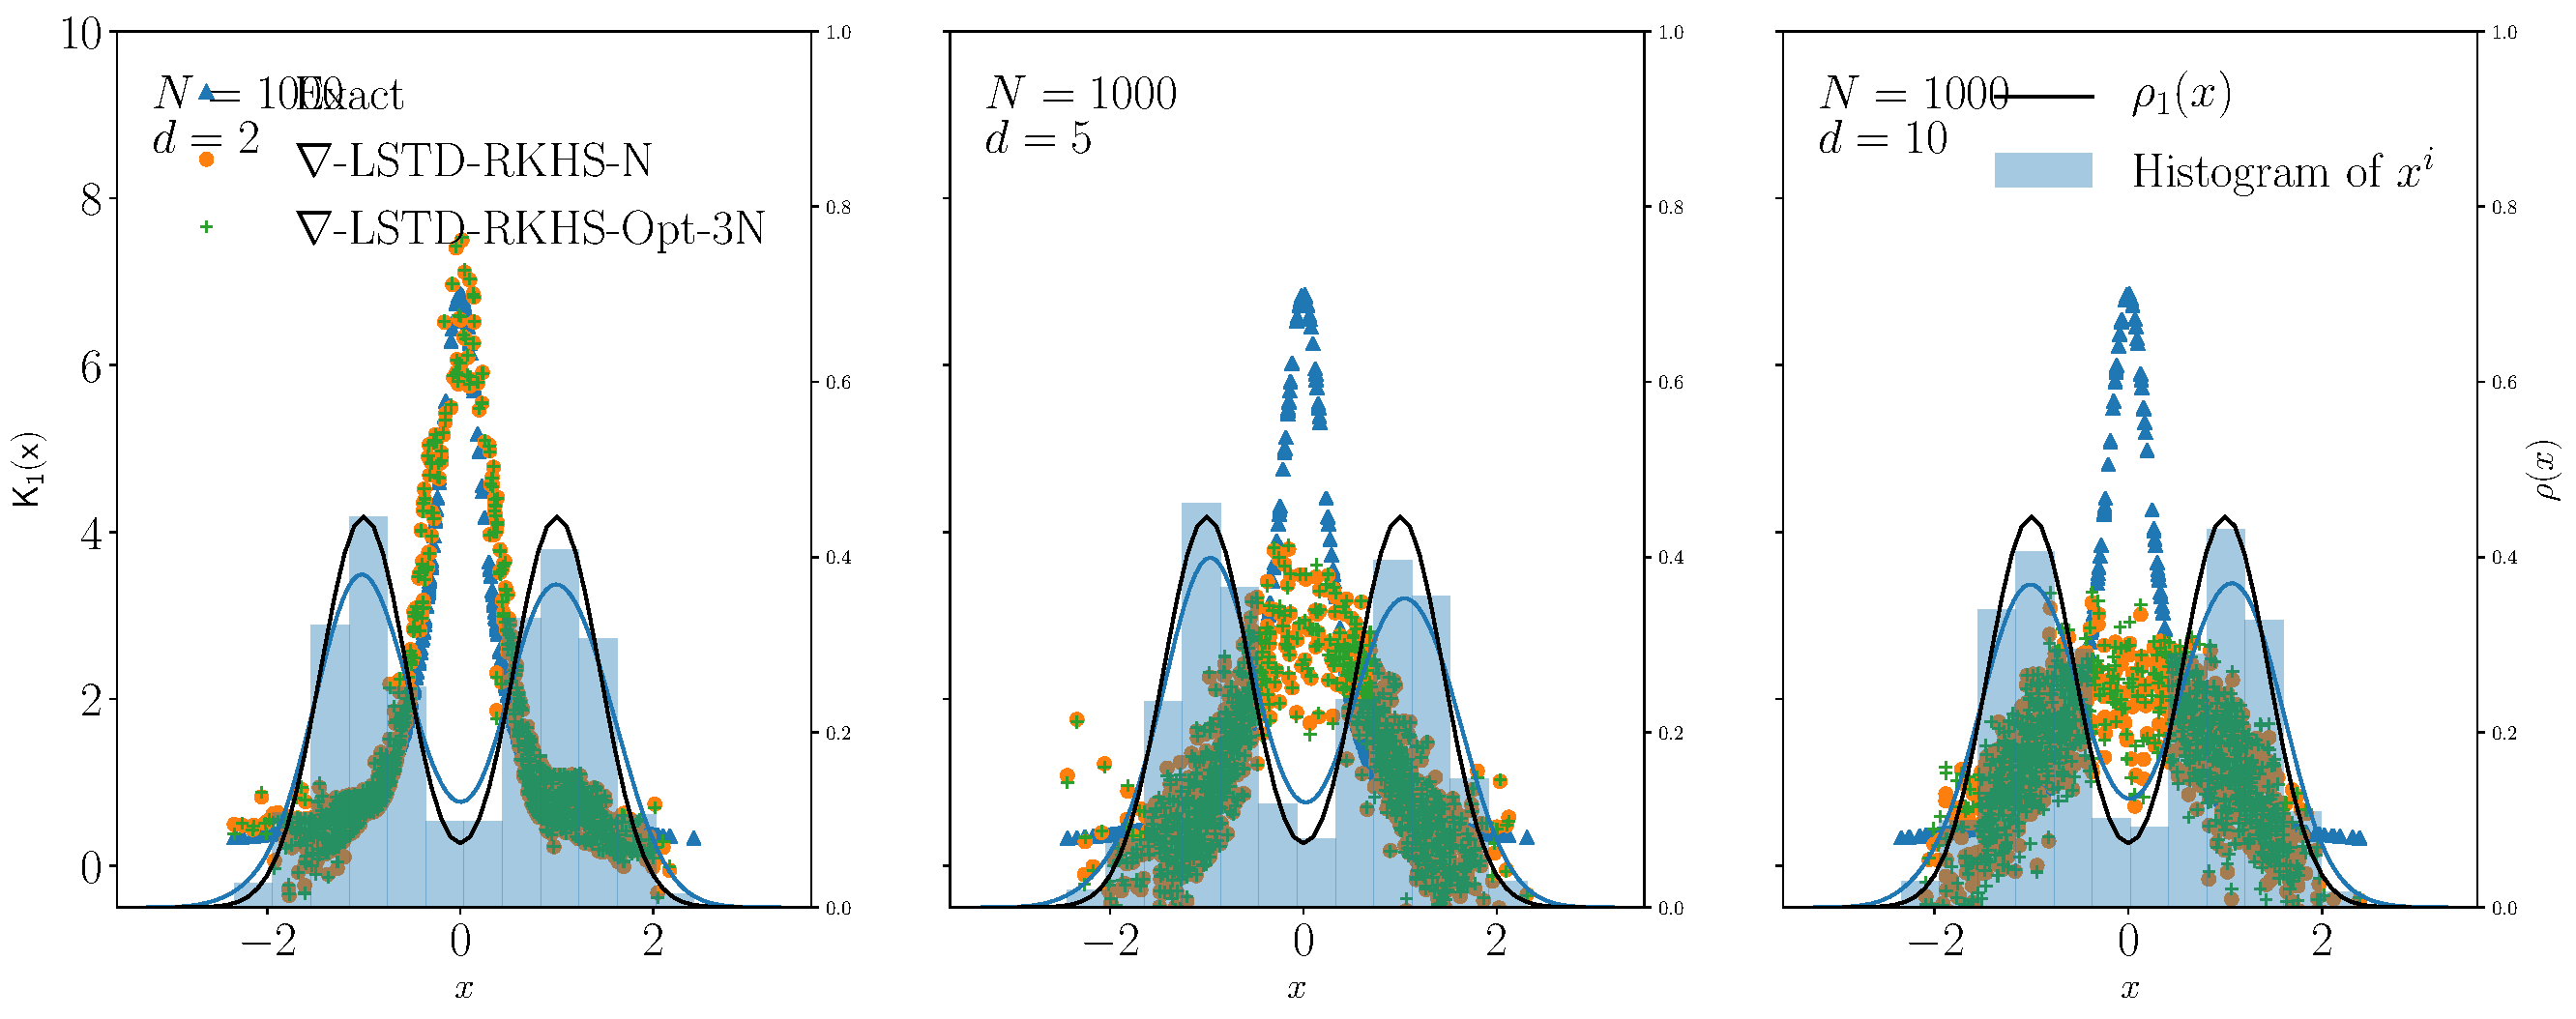
\includegraphics[width=6in]{images/Chap4_gain_N_dN_d2510}} 
	}
	\mbox{
		\subfigure [] {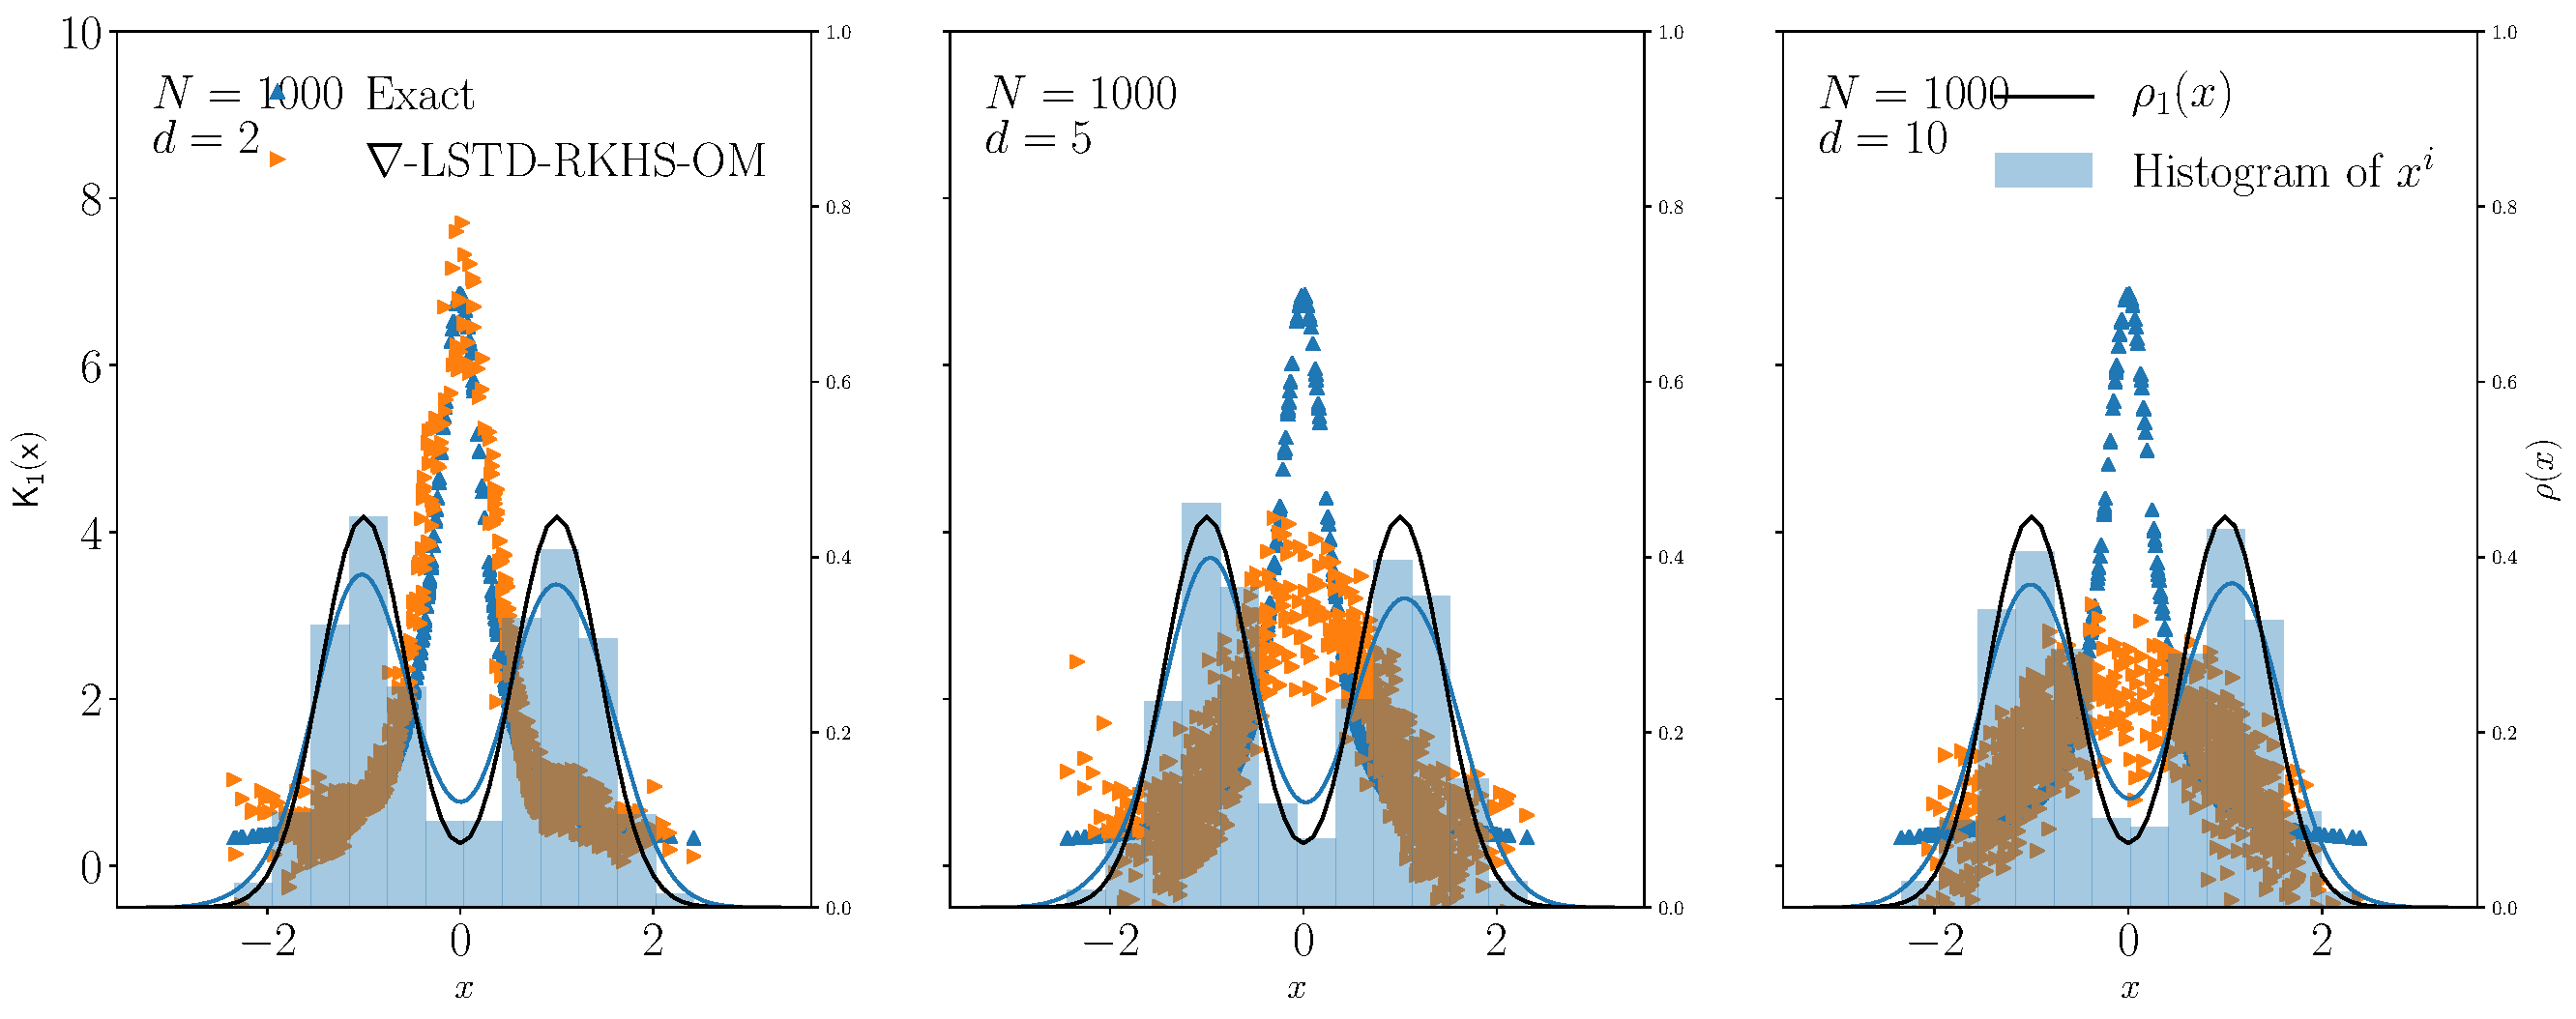
\includegraphics[width=6in]{images/Chap4_gain_om_d2510}} 
	}
	\mbox{
		\subfigure [] {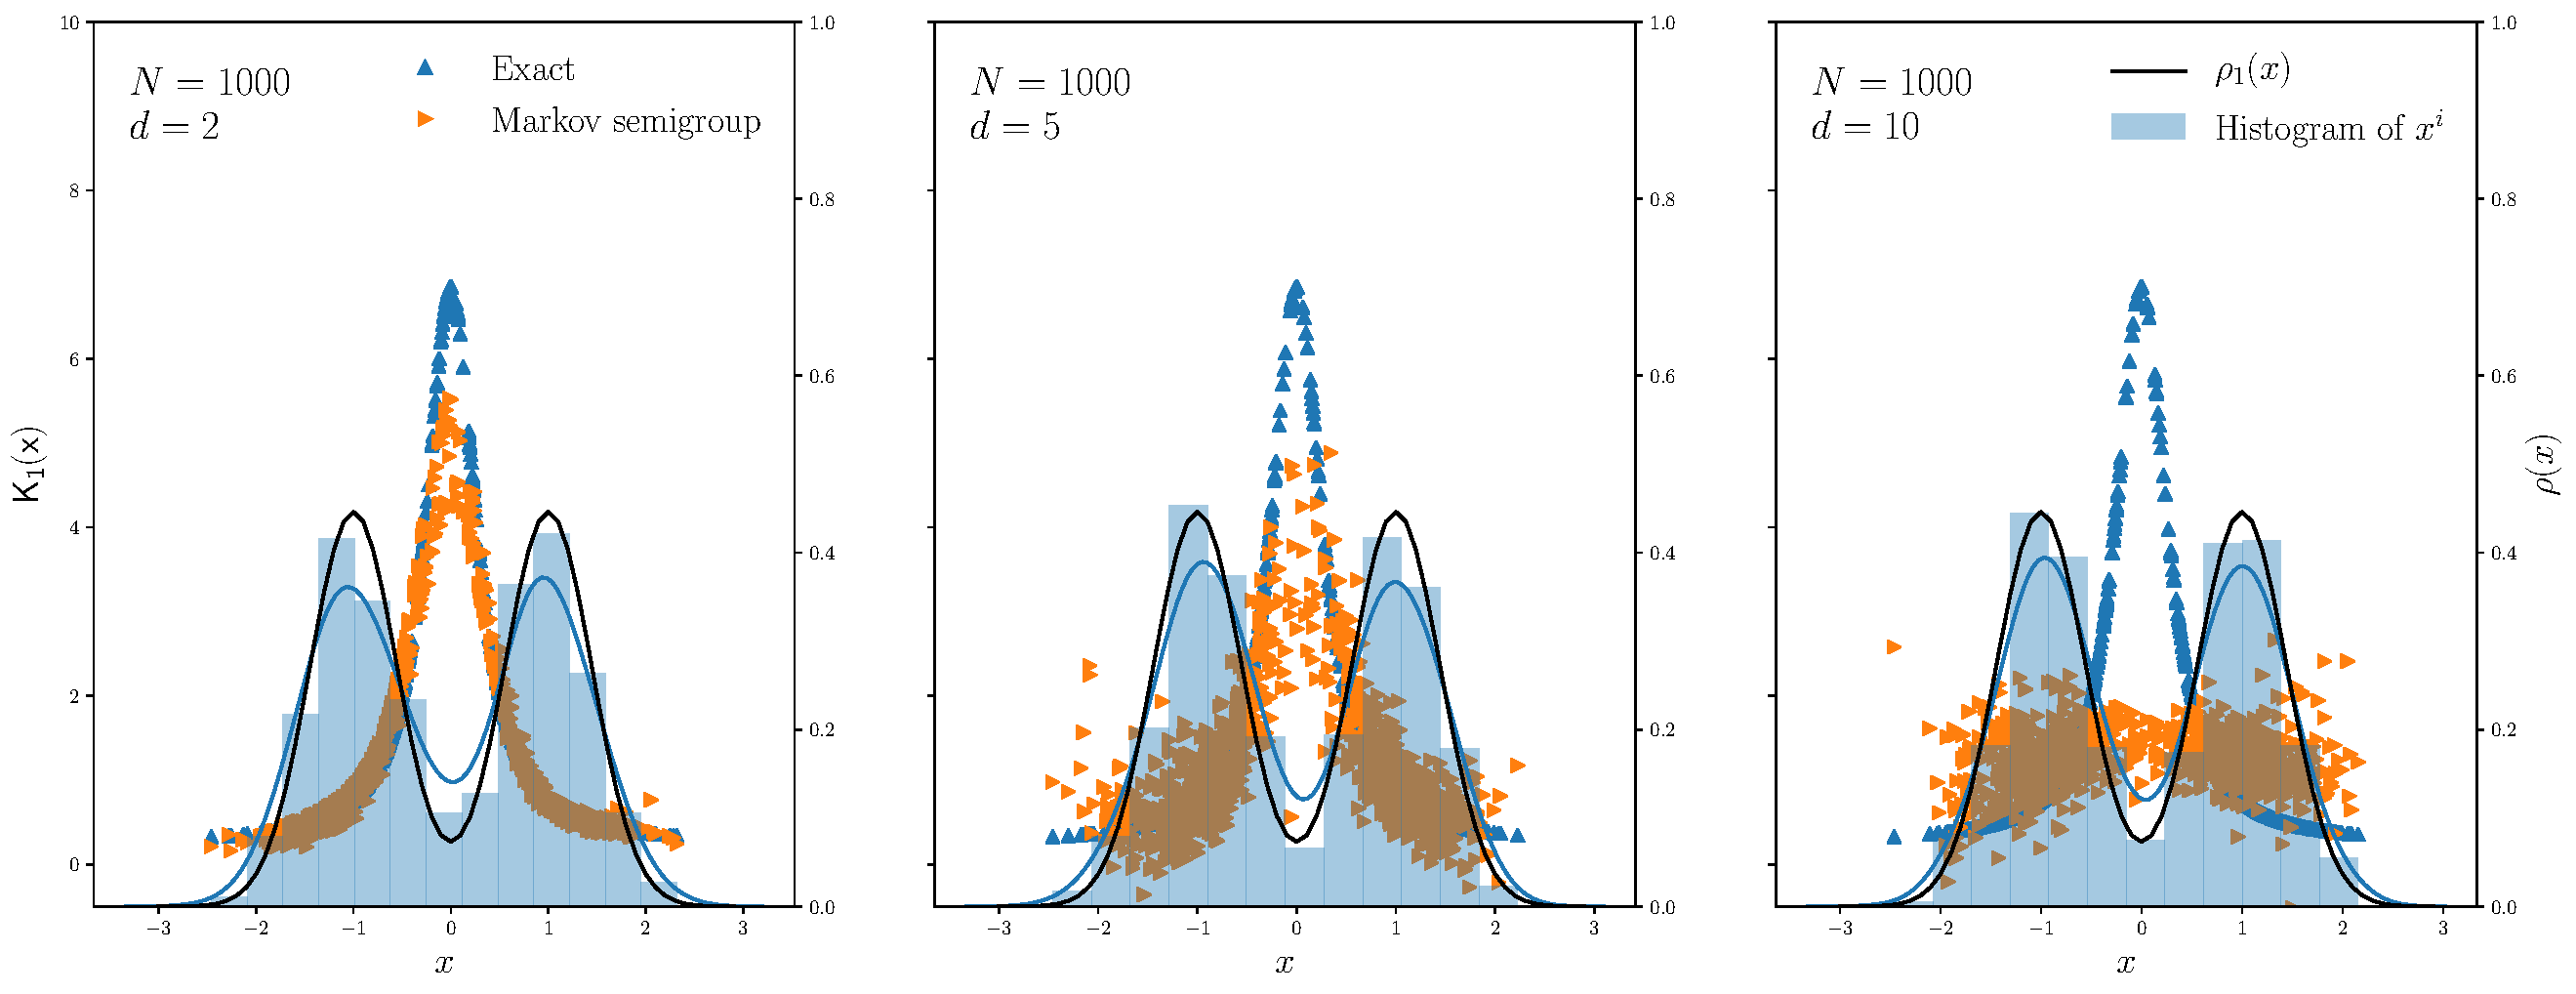
\includegraphics[width = 6in]{images/Chap4_gain_coif_d2510}} 
	}
	\caption[RKHS and coifman performance]{Gain function approximations A) RKHS optimal and RKHS simplified with $2N$ and $N$ parameters respectively \cite{radmey18a}, B) RKHS-OM method \cite{radmey19}, C) Markov semigroup approximation \cite{tagmeh16}.}
	\label{fig:diff_td_rkhs_coif_d2510}
\end{figure}

\begin{figure}[htbp]
	\centering
	\mbox{
		\subfigure [] {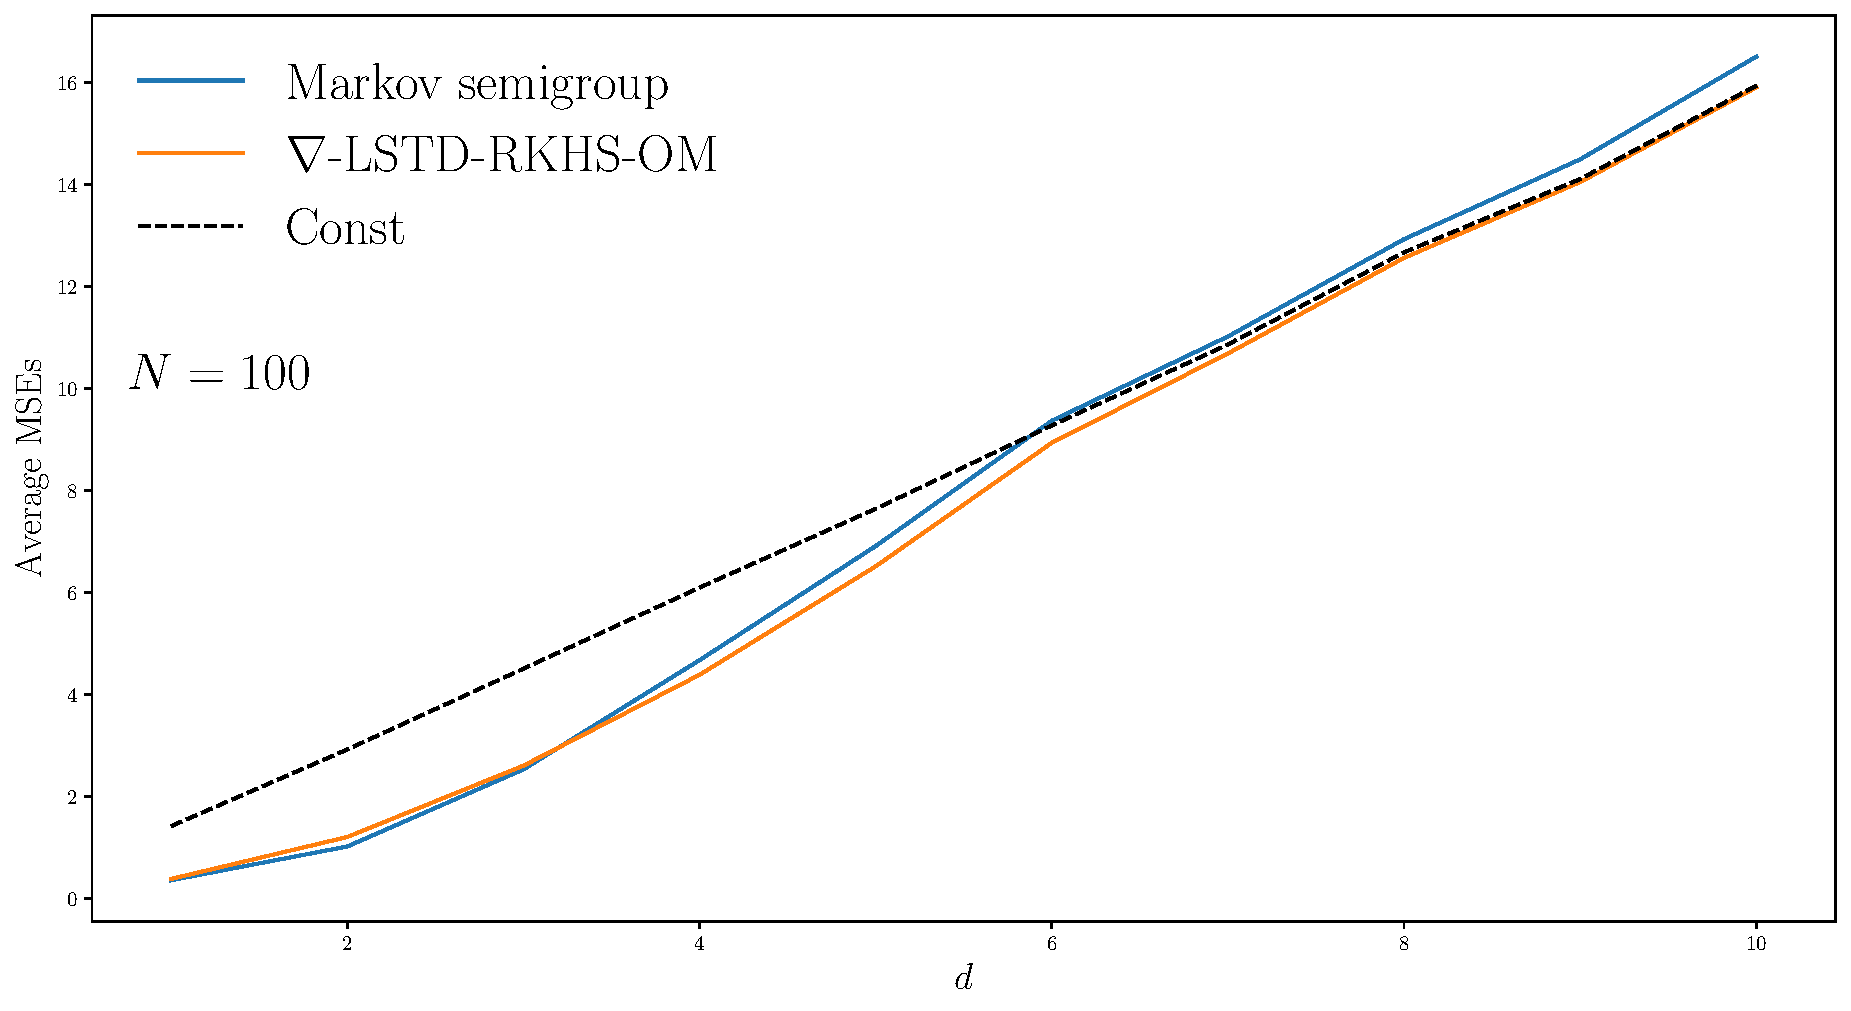
\includegraphics[width=4.5in]{images/Chap4_logMSEvdforN100}} 
	}
	\mbox{
		\subfigure [] {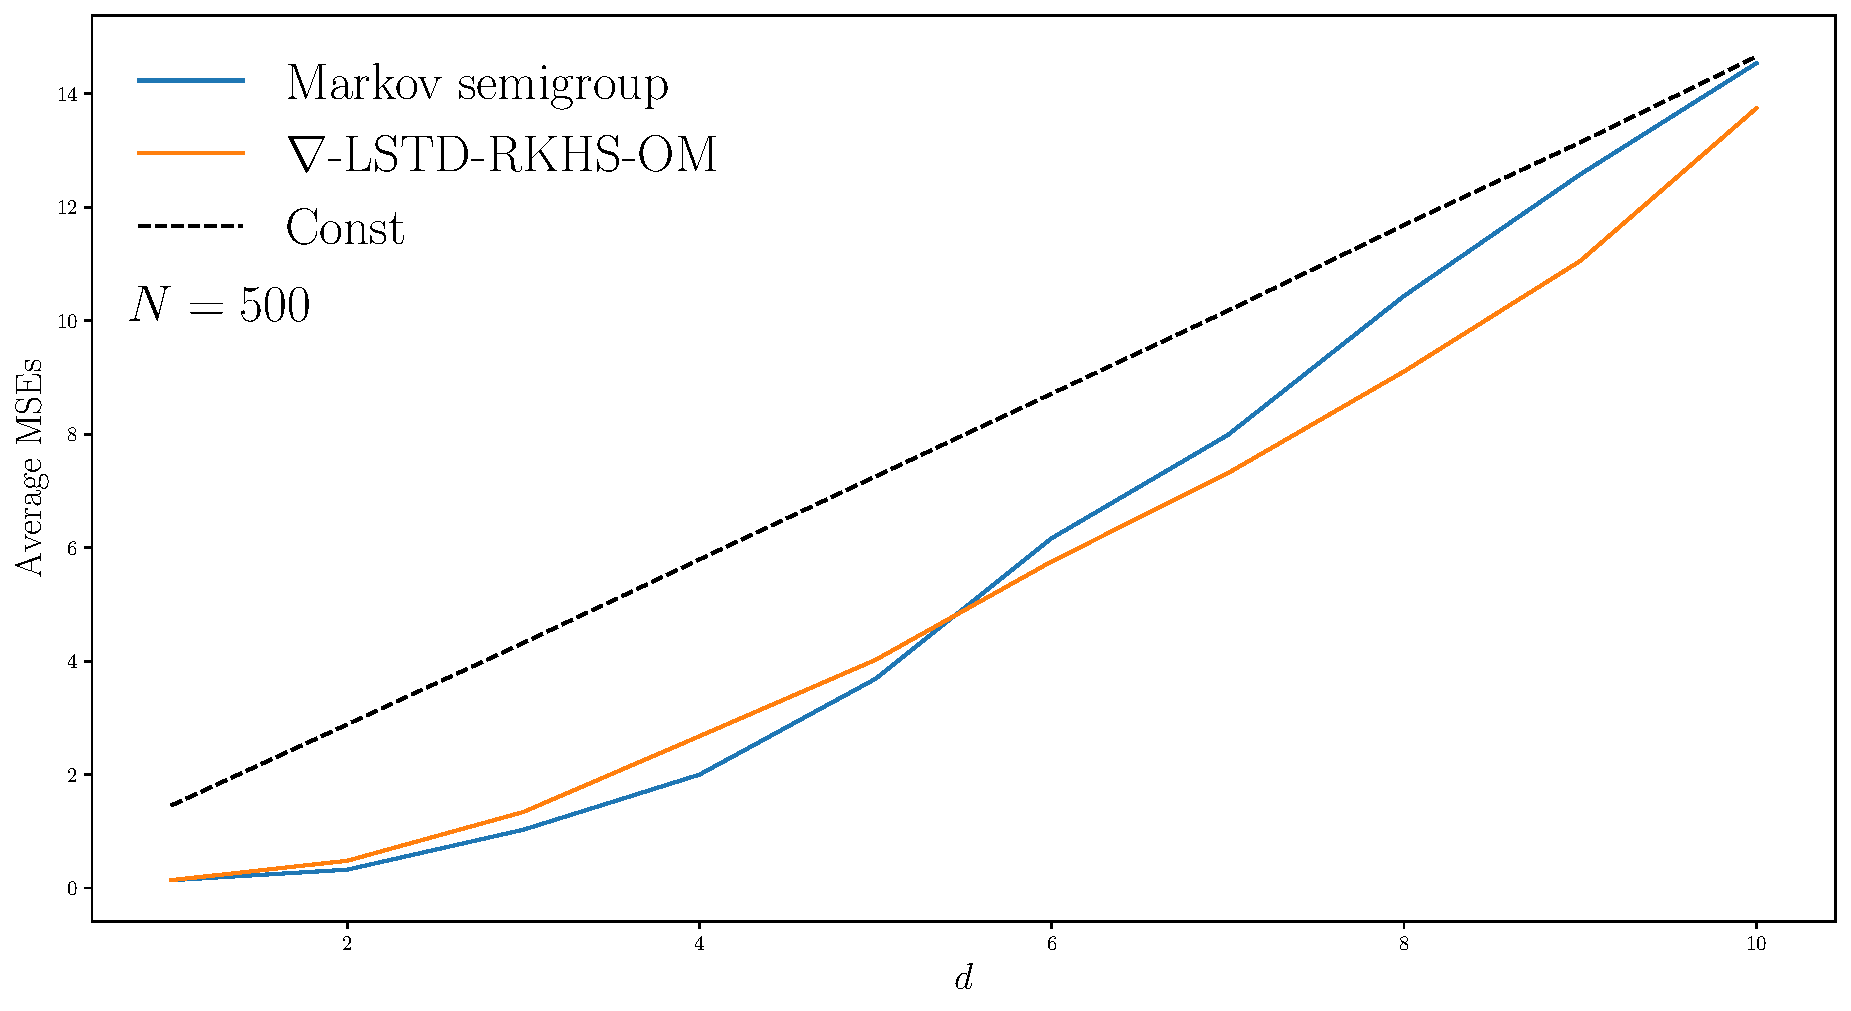
\includegraphics[width=4.5in]{images/Chap4_logMSEvdforN500}} 
	}
	\mbox{
		\subfigure [] {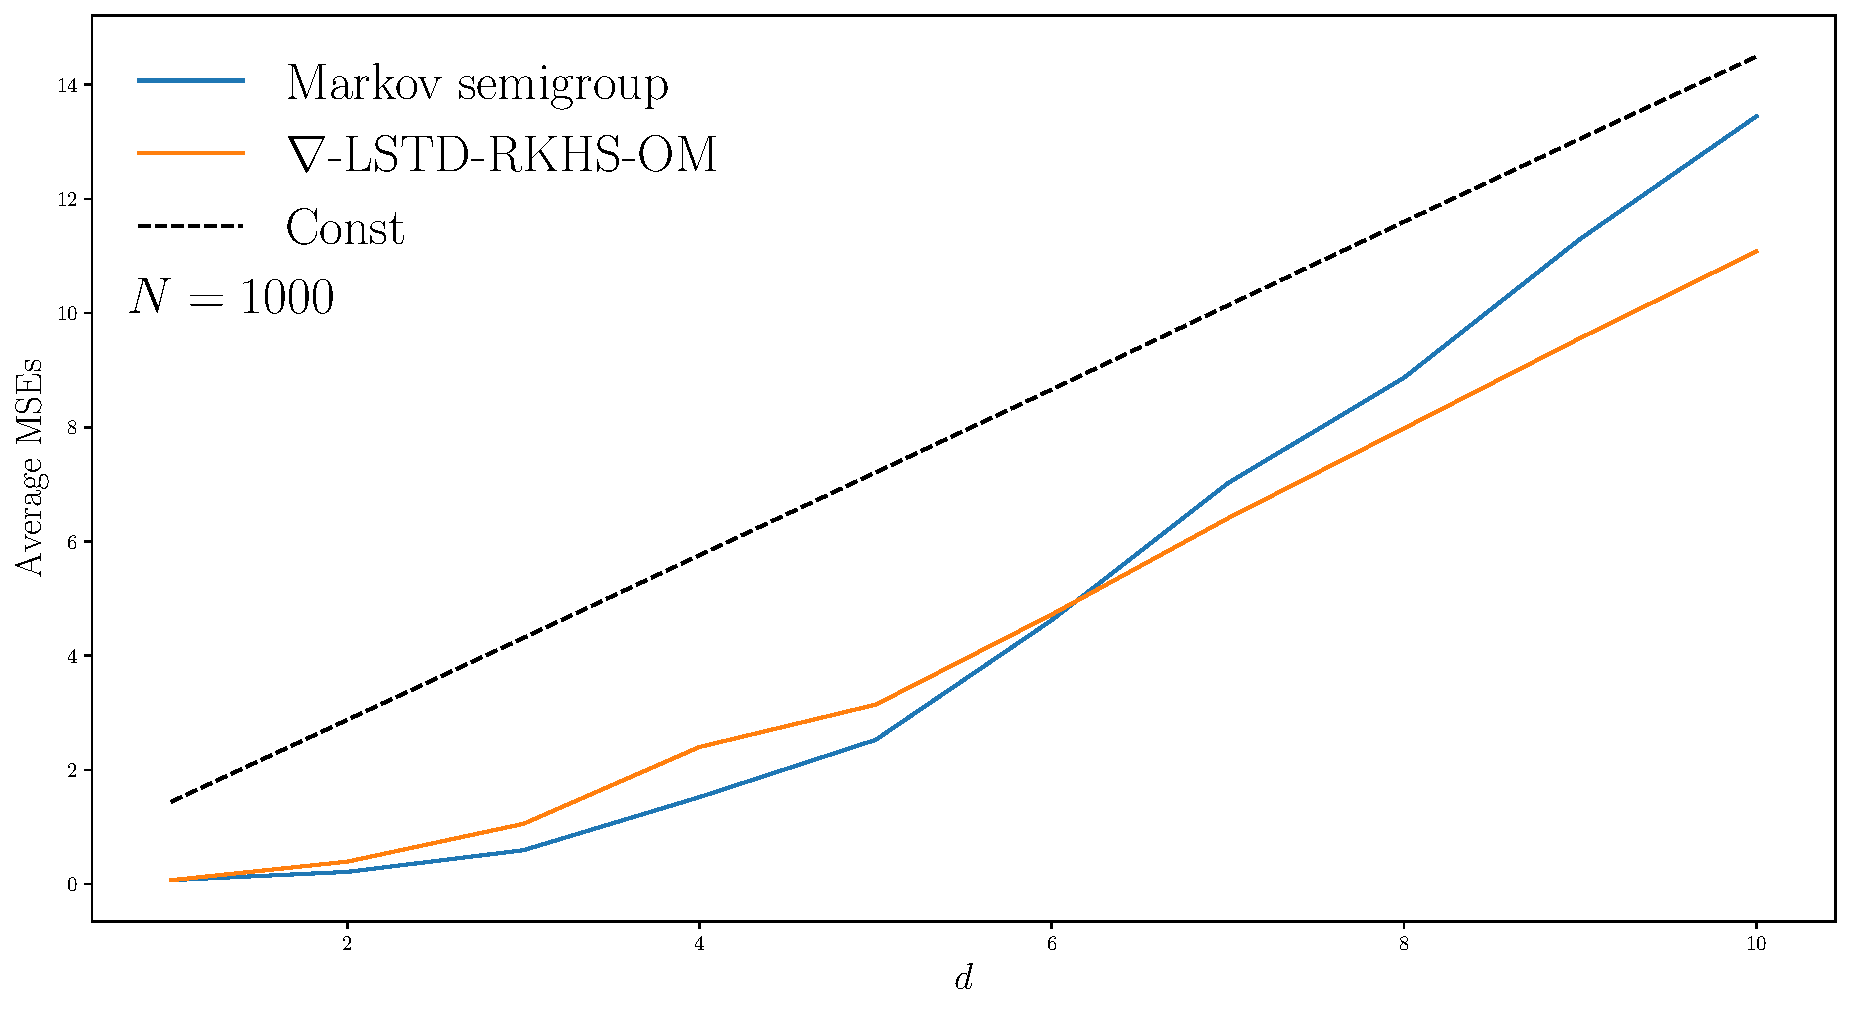
\includegraphics[width = 4.5in]{images/Chap4_logMSEvdforN1000}} 
	}
	\caption[RKHS and coifman performance]{Gain function approximations A) RKHS optimal and RKHS simplified with $2N$ and $N$ parameters respectively \cite{radmey18a}, B) RKHS-OM method \cite{radmey19}, C) Markov semigroup approximation \cite{tagmeh16}.}
	\label{fig:diff_td_rkhs_coif_d2510}
\end{figure}

\Fig{fig:diff_td_linear} compares the performance of the various choices of basis functions for different simulation times $T = 10^4, 10^5, 10^6$ of the Langevin SDE. An Euler-discretization scheme was implemented with time-step size of $\delta = 0.01$. A $10$-dimensional basis was chosen in each case. The true FPF gain computed using the integral formula \eqref{e:fpf_gain_1d} is also plotted for comparison. The histogram of the particles $\{x^i\}$ obtained from the SDE and the true density $\pr$ are shown as the shaded region. As expected, the accuracy of the approximation improves as $T$ increases. For $T=10^6$, the histogram converges to $\pr$ and as a result, the gain approximation matches well with the true value. Although, the approximation is not tight everywhere, the accuracy is typically better at values of $x$ for which $\pr(x)$ is large. All three choices of basis functions perform nearly similar. Polynomials weighted by the component densities $\pr_i$ is a better choice because it ensures that the gain decays at large values of $x$. 

\Fig{fig:diff_td_rkhs_coif} compares the performance of the various basis-free approaches for the same density $\pr$ for $N = 100,500,1000$. The particles $\{x^i\}_1^N$ distributed according to $\pr$ can be thought of as being available from the FPF. The parameter $\epsy$ was set to $0.1$ in the Markov semigroup approximation method (the best value found in \cite{tagmeh16a}). \Fig{fig:diff_td_lang_linear} shows the approximations obtained using the same weighted polynomial basis, but using the Langevin-specific $\gradTD$ algorithm in \Section{s:diff_td_langevin}. The same seed was used for random number generation in each of the implementations. It is important to recall that these methods do not require simulating the Langevin SDE. It can be seen from Figures \ref{fig:diff_td_linear}, \ref{fig:diff_td_lang_linear} and \ref{fig:diff_td_rkhs_coif} that these methods show superior performance over those requiring the SDE simulation. Also, the number of particles required for a good approximation of the gain reduces dramatically from $T=10^6$ to $N=500$. Moreover, they make intelligent use of the FPF particles, whereas the other methods derive no useful information from them.   

Another surprising observation in \Fig{fig:diff_td_rkhs_coif} A is that the optimal RKHS solution with $2N$ parameters and the reduced complexity solution with $N$ parameters produce an identical gain estimate. This holds true even for higher dimensional examples with $d\leq 5$ (See \Fig{fig:diff_td_rkhs_coif_d2510}). The RKHS-OM solution is better, especially at particle locations closer to the boundaries. \Fig{fig:beta_comparison} compares the magnitudes of the optimal parameter estimates obtained from the three algorithms. Parameters $\beta_i^\circ$ corresponding to the reduced complexity solution tend to take higher values than $\beta_i^*$ or $\beta_i^{OM}$ and are susceptible to numerical instabilities. RKHS-OM algorithm is the preferred choice, as its computational complexity is comparable to the reduced complexity solution, but is much more stable numerically. 

The mean square error in the approximation is computed as:
\begin{equation}
\mathcal{E} \eqdef \frac{1}{N} \sum_{i=1}^N \|\kFPF(x^i)  - \hat{\kFPF}(x^i) \|^2,
\label{e:gain_mse}
\end{equation}
where $\hat{\kFPF}$ denotes the approximate gain. \Fig{fig:hist_mse} displays the histograms of the MSE obtained for $N=1000$ for $100$ independent trials. As expected, the RKHS-OM and the Markov semigroup approximation methods have the lowest approximation error. All the methods however, produce significant improvement over the constant gain. 

\subsection*{Higher dimensional example}
It is of interest to test how the gain approximation methods scale with the system dimension $d$. We considered higher dimensional examples with $1<d \leq 10$.  
The $d$ dimensional probability density is composed as a product of $d$ independent 2-component Gaussian mixtures along each dimension. Let $\pr_i$ be the density in the $i^{\text{th}}$ dimension and let $\pr$ be defined as 
\begin{equation}
\pr(x) = \prod_{i=1}^d \pr_i(x_i),
\end{equation}
where $x \eqdef [x_1, x_2, \cdots, x_d] \in \Re^d$. 
Taking $\log$ on both sides, the potential function is expressed as a sum:
\begin{equation}
U(x) = \sum_{i=1}^d U_i(x_i)
\end{equation}
where $U = -\log(\pr)$.
Then,
\begin{equation}
\nabla U = \Bigl[ \frac{\partial U_1}{\partial x_1}, \frac{\partial U_2}{\partial x_2}, \cdots , \frac{\partial U_d}{\partial x_d} \Bigr]
\end{equation}
The FPF gain $\kFPF$ consists of $d$ components and can be written in terms of the solution to Poisson's equation $h$ as: 
\begin{equation}
\begin{aligned}
\kFPF &= \Bigl[\frac{\partial h}{\partial x_1}, \frac{\partial h}{\partial x_2}, \cdots \frac{\partial h}{\partial x_d}\Bigr] \\
& = \Bigl[ \kFPF_1, \kFPF_2, \cdots, \kFPF_d\Bigr],
\end{aligned}
\end{equation}
and, 
\begin{equation}
\Delta h = \sum_{i=1}^d \frac{\partial^2 h}{\partial x^2_i} = \sum_{i=1}^d \frac{\partial \kFPF_i}{\partial x_i}
\end{equation}
Suppose, it is possible to decompose the observation function in the form, $c(x) = c_1(x_1) + c_2(x_2) + \cdots + c_d(x_d)$, then the Poisson's equation to obtain the FPF gain function becomes:
\begin{equation}
- \sum_{i=1}^d \frac{\partial U_i}{\partial x_i} \kFPF_i(x_i)+ \sum_{i=1}^d \frac{\partial \kFPF_i(x_i)}{\partial x_i} = -\sum_{i=1}^d \tilde{c_i}(x_i)
\label{e:fpf_multi}
\end{equation}
This can be split into $d$ independent Poisson's equations as follows:
\begin{equation}
-\frac{\partial U_i}{\partial x_i} \kFPF_i(x_i) + \frac{\partial \kFPF_i(x_i)}{\partial x_i} = -\tilde{c_i}(x_i) \,\qquad\,  1 \leq i \leq d. 
\end{equation}
In particular, we consider $c(x) = C^\transpose x$, where $C =\mathbf{1}$. 

\Fig{fig:diff_td_rkhs_coif_d2510} compares the performance of the various methods for $d=2,5,10$ for $N=1000$. The performance degrades with $d$ as expected. This is partly because $N=1000$ is insufficient for larger values of $d$.   
\subsection{Nonlinear oscillator}
\label{s:nl_oscillator}
We consider next the nonlinear oscillator example introduced in \cite{yanmehmey13}.
The state evolves on the unit circle, and the observations are nonlinear:
\begin{equation*}
\begin{aligned}
\ud \oscState &= \omega \ud t+\sigma_{B}\ud B_t \quad \text{mod }2\pi,
\\
\ud Z_t &= c(\oscState)\ud t+ \sigma_{W} \ud  W_t
\end{aligned}
\end{equation*}
The parameter $\omega$ is  the
mean angular velocity,  and $\bfmB$ and $\bfmW$ are mutually independent standard Brownian motions.
The observation function is
$c(\oscState)=\frac{1}{2}[1+\cos(\oscState)]$. Nonlinear oscillators have important applications including neuroscience. 

The feedback particle filter for this model is given by :
\begin{equation*}
\ud \oscState^{i}_t = \omega \ud t +\sigma_{B}\ud B^{i}_t+\kFPF(\oscState^{i}_t) \circ \ud I^i(t)  \quad  \text{mod }2\pi\, ,
\end{equation*}
with $\ud I^i(t) = \ud Z_t-\frac{1}{2}(c(\oscState_t^{i})+\hac_t)\ud t$.
The gain function $\kFPF(\oscState,t)$ at each instant $t$ is obtained as the solution to \eqref{e:diff_td_poissons}:
\begin{equation*}
- U'(\oscState) \kFPF(\oscState) + \kFPF'(\oscState) = -\frac{\tilc(\oscState)}{\sigma^2_W}  %\qquad \{\tilc =c-\int c(\oscState)\pr(\oscState,t)d\oscState\}
\end{equation*}
The conditional density $\pr(\oscState,t)$ at any instant is modeled as a mixture of von Mises densities:
\begin{equation*}
\pr(\oscState)=\sum_{i=1}^{m}w_{i}\pr_i(\oscState)
\end{equation*}
Each component of the mixture $\pr_i(\oscState)$ is given as follows:
\begin{equation*}
\pr_i(\oscState,t) =  \beta^{-1} \exp  \bigl( \kappa_i \cos(\oscState-\mu_{i} )    \bigr),
\end{equation*}
where $\beta$ is a normalizing constant, and $\mu_{i}$ is the mean of the density. This reduces to   a uniform density for $\kappa_{i}=0$, and the variance vanishes as $\kappa_{i}\to \infty$ \cite{haspea00}. By choosing a family of a mixture of von Mises densities, it is possible to model any form of circular density from uniform to a bimodal Gaussian mixture.
Poisson's equation can be numerically solved in the scalar case for this mixture density $\pr(\oscState)$, so that the gain function $\kFPF$ is numerically computed.
% \iffalse

\subsubsection*{Linear parameterization}
We consider a mixture of von Mises densities with the following parameters: $\mu_1 = -\pi/3$,\ \
$\mu_2 = \pi/3$,\ \
$\kappa_1=\kappa_2=3$,\ \
$w_1 =0.5$,\ \
$w_2 =0.5$.


The $\nabla$-LSTD learning algorithm is applied to this nonlinear oscillator problem. A linearly parameterized family using sines and cosines is the chosen basis. This is a reasonable choice because for a uniform density, the gain $\kFPF=-\frac{\sin \oscState}{2\sigma_{W}^{2}}$.

\begin{figure*}
	\Ebox{.9}{images/Chap4_nl_oscillator_be}
	\caption{Comparison of $\nabla$-LSTD learning with Bellman error minimization for $4,6$ and $8$ dimensional Fourier basis for a nonlinear oscillator model}
	\label{fig:gain_nl_oscillator}
\end{figure*}

For comparison, we also considered an approximation computed by minimizing the $L^2(\pr)-$norm of the Bellman error:
% \begin{equation*}
\begin{align}
\min_{\param}\|\clE(\param)\|_{L^2}^{2}=\min_{\param}\langle \clD h^\param + \tilc \rangle_{L^2} = \min_{\param}\|\clD h^\param +\tilc \|_{L^2}^{2}
\label{e:fpf_nl_be}
\end{align}
% \end{equation*}
This minimization problem can be solved using Monte-Carlo methods.

\Fig{fig:gain_nl_oscillator} compares the performance of the $\nabla$-LSTD learning algorithm and the Bellman error minimization algorithm with the numerically computed exact gain function for basis functions of dimensions $4$, $6$ and $8$. It can be observed that $\nabla$-LSTD learning gives a better approximation than the $BE$ minimization algorithm in regions of high values of $\pr(\oscState)$.

\subsection{Filtering experiments}
\label{s:filtering_experiments}
The examples surveyed in this section are the following:
\begin{itemize}
	\item A parameter estimation problem with linear observations and bimodal prior
	\item A nonlinear multidimensional ship dynamics model.
\end{itemize}
\subsection{Parameter estimation }
\label{s:param_estimation} \anand{needs more work in terms of better plots}
A simple example where the state $X_t \in \Re$ remains at its initial value is considered first.
State-observation model:
% This experiment has been performed in \cite{tagmeh16a}, \cite{raddevmey16} and \cite{radmey18a}.
\[
\begin{aligned}
\rmd X_t&=0, \qquad X_0 \sim \rho_0\\
\rmd Z_t&= X_t \rmd t+\sigma_{W}\rmd W_t,
\end{aligned}
\]
where the measurement noise standard deviation is $\sigma_{W} = 1$. 
In this simple example, the filtering problem reduces to parameter estimation. It is observed in \cite{arumasgorcla02} that conventional particle filters are not well suited for such parameter estimation problems, where there is no state dynamics or process noise.
%\textbf{Comparisons of gain approximation}
%\Fig{f:gain_comparison} shows gain magnitudes for $t=0$,  plotted at each of the $500$ particle locations $\{x^i_0\}$; the five plots correspond to the five computational approaches. The Markov semigroup approximation and the RKHS based methods tend to approximate the gain function much better than a finite dimensional basis.
%
%\begin{figure}[htbp]
%	\centering
%	\Ebox{0.9}{images/Chap4_gain_2gmm_compare}
%	\vspace{-0.5em}
%	\caption{Gain approximations obtained by the various algorithms at $t=0$.}	\vspace{-0.02in}
%	\label{f:gain_comparison}
%\end{figure}
\subsection*{Online gain estimation}
To compute the exact gain using \eqref{e:fpf_gain_1d}, a smooth approximation to the posterior density $\pr_t$ is required for all $t$. This was done by assuming that the particles are generated from a  3-component Gaussian mixture density. Based on this model, the parameters for the density were obtained using the EM algorithm.

The constant gain approximation FPF  version was compared previously in \cite{tilghiomeh13} with the extended Kalman filter (EKF) and the  sequential importance resampling (SIR) particle filter. The prior density for the EKF was chosen to be a Gaussian with matching mean and covariance to the actual bimodal prior. The SIS-PF was   initialized with $1000$ particles drawn i.i.d from $\pr_0$.

Many variants of SIS-PF were tested in these experiments.
Particle degeneracy was observed in implementations without resampling.
Resampling at regular intervals was implemented to address this, but
numerical issues persisted due to lack   of diversity of particles. The comparisons
shown
here are for SIS-PF with periodic resampling at every third time interval.

\begin{figure}[htbp]
	\centering
	\mbox{
	\subfigure [] {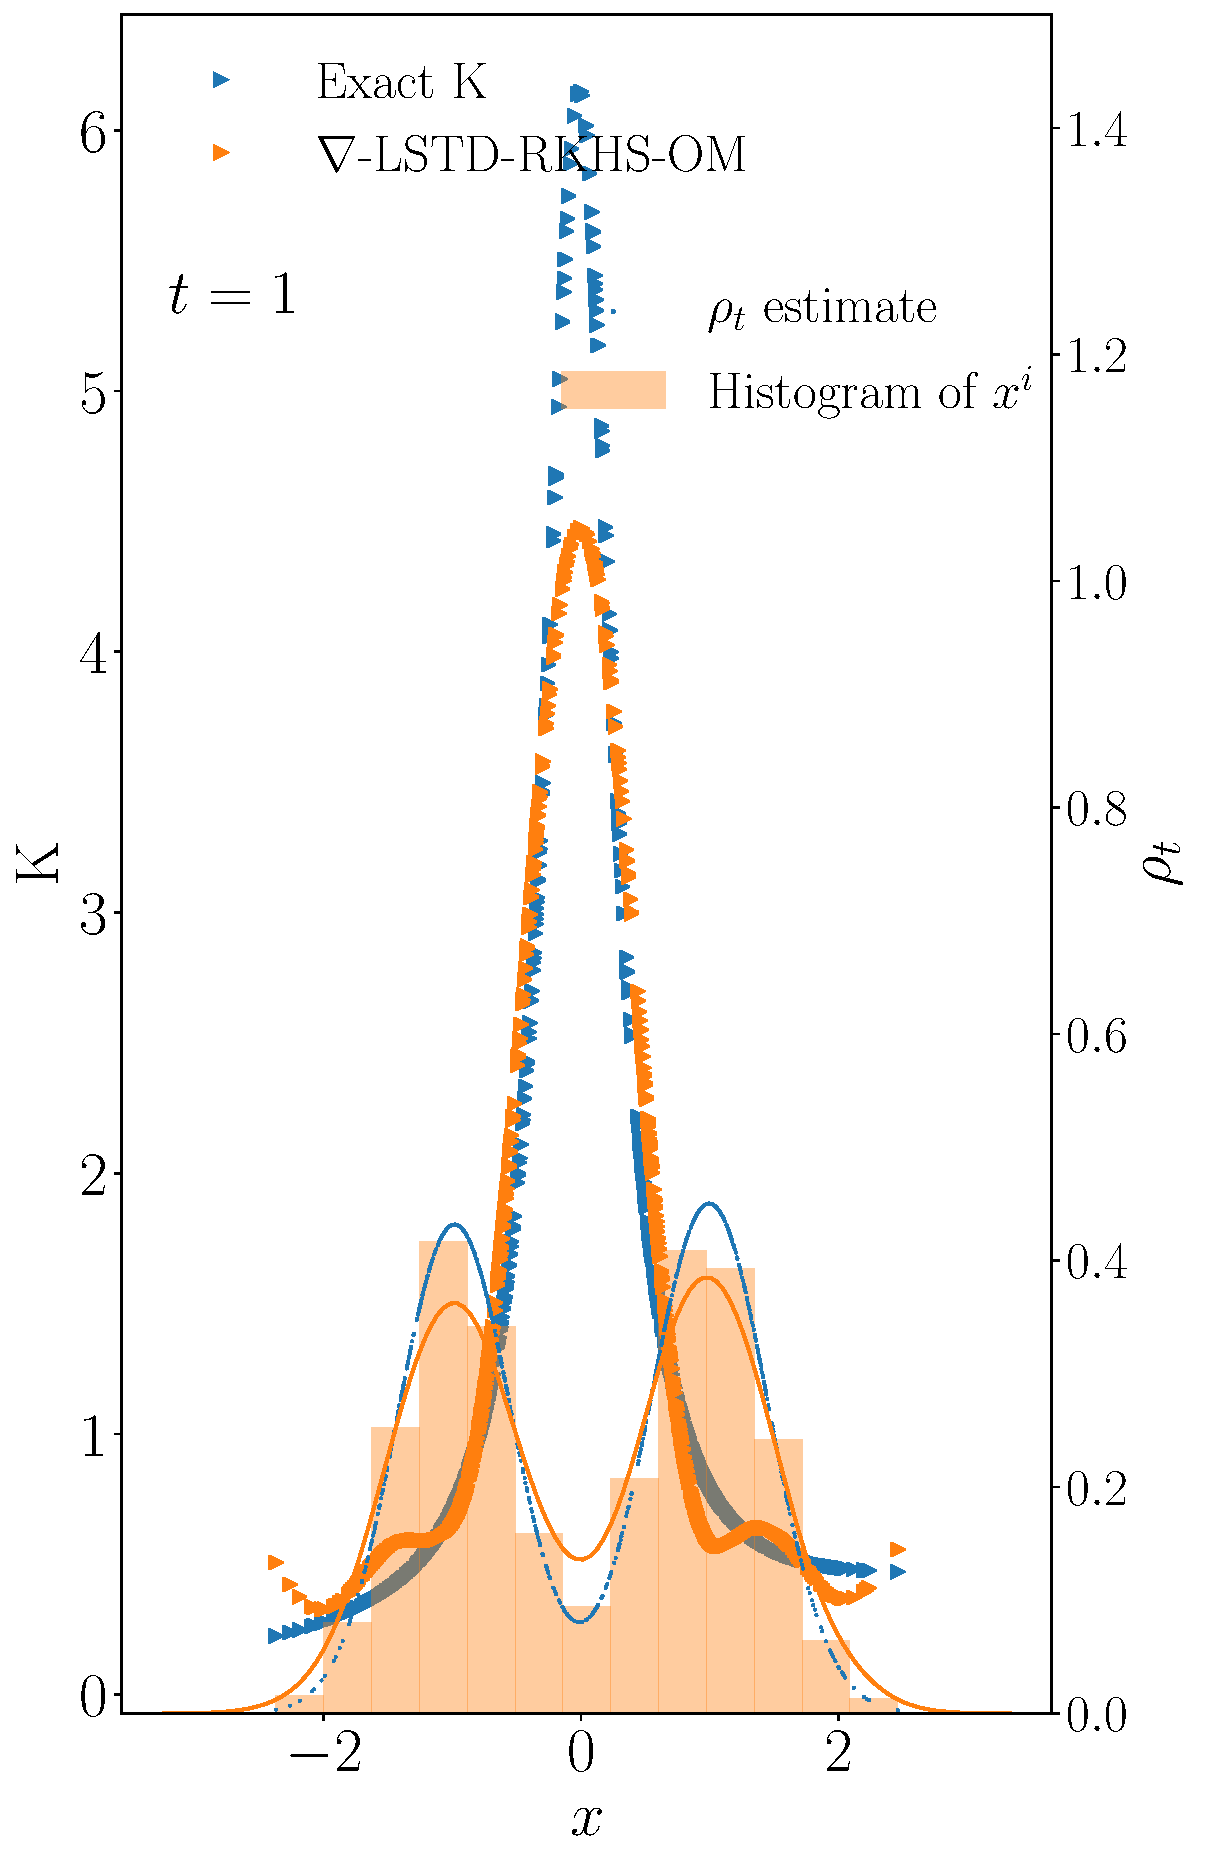
\includegraphics[width=2in]{images/Chap4_gain_posterior_exact_om_t_1}} 
	\subfigure [] {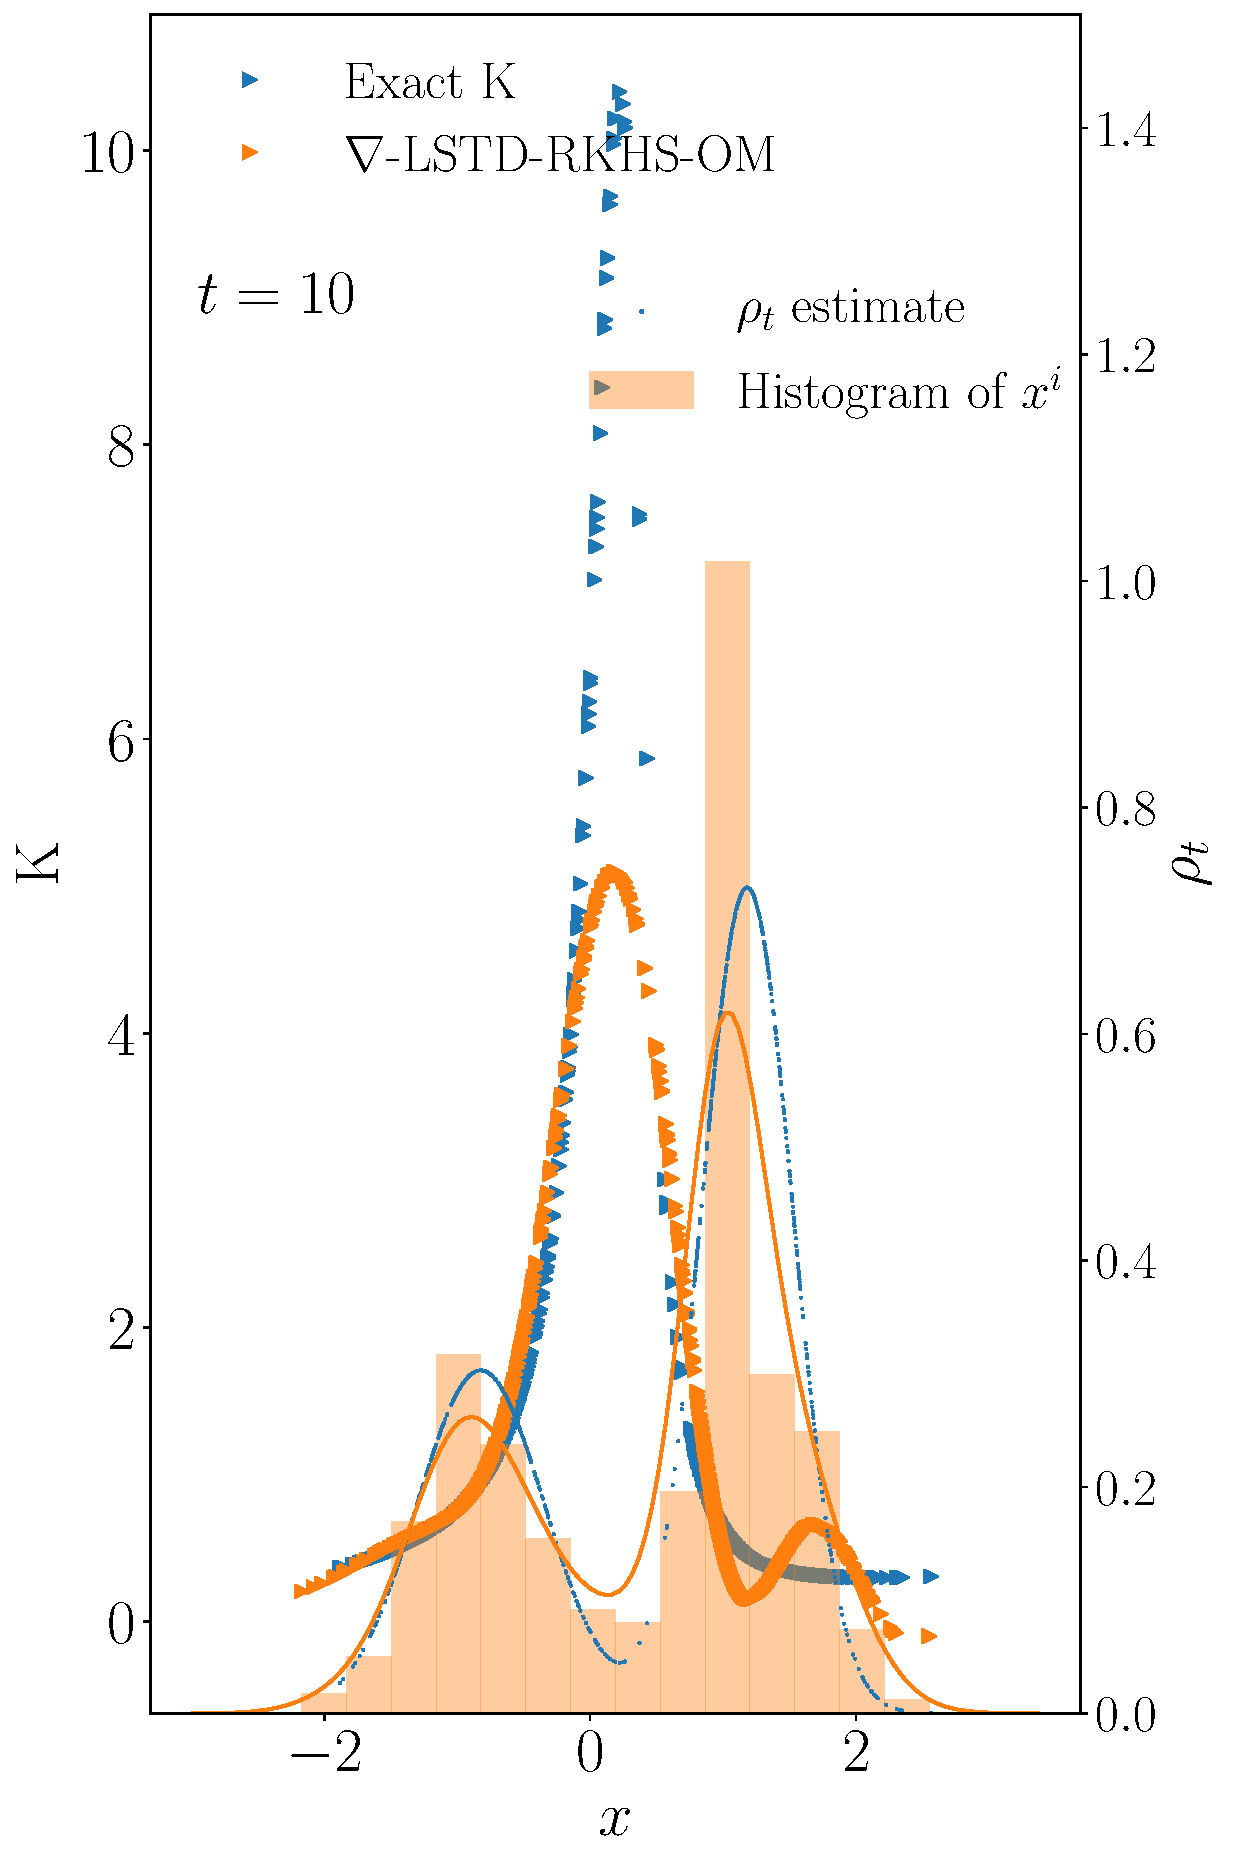
\includegraphics[width=2in]{images/Chap4_gain_posterior_exact_om_t_10}} 
	\subfigure [] {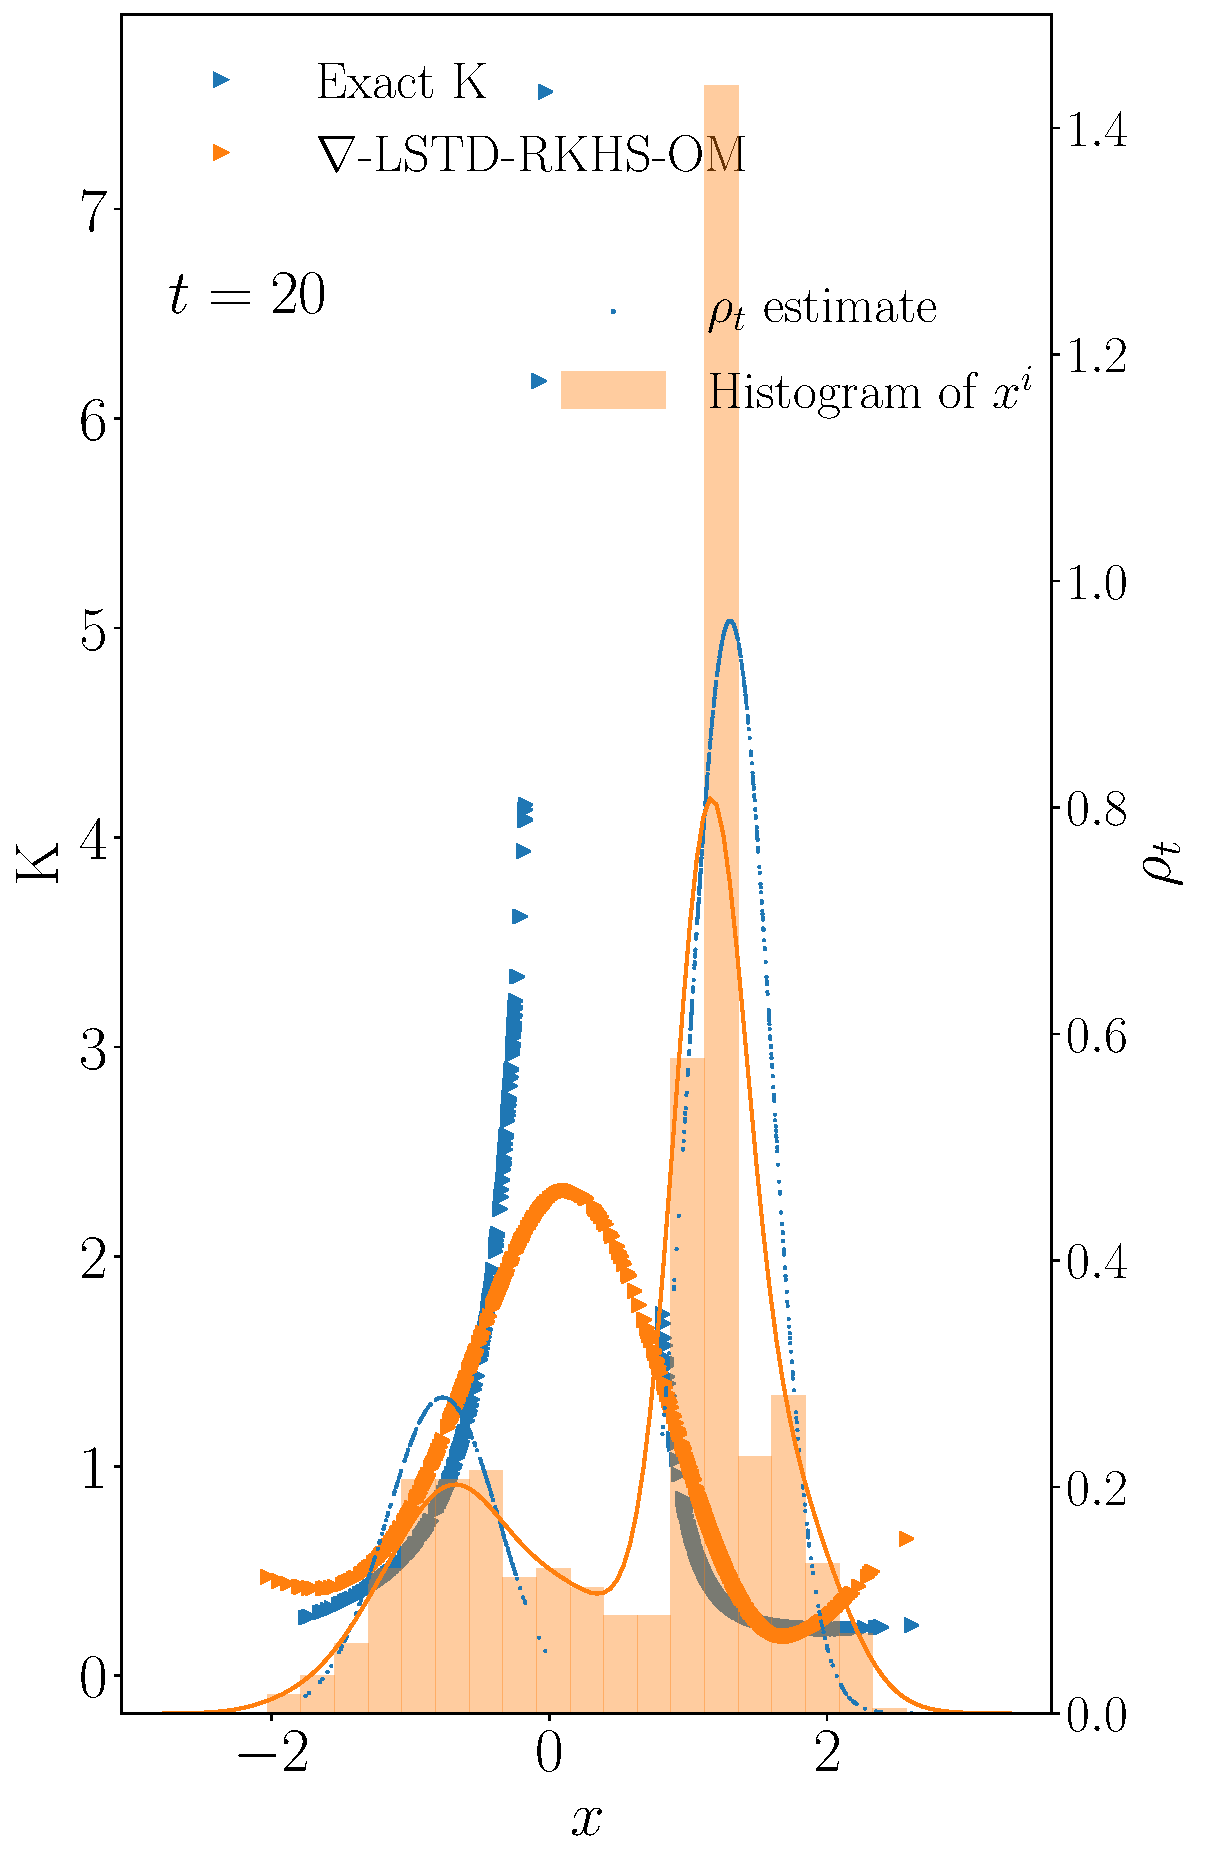
\includegraphics[width=2in]{images/Chap4_gain_posterior_exact_om_t_20}} 
	}
	\caption{ Gain approximations and posterior estimates at $t=1,10$ and $20$ respectively using i) exact computation ii) $\gradTD$-RKHS-OM method}
	\label{fig:gain_hist_11020}
\end{figure}

\begin{figure}[htbp]
	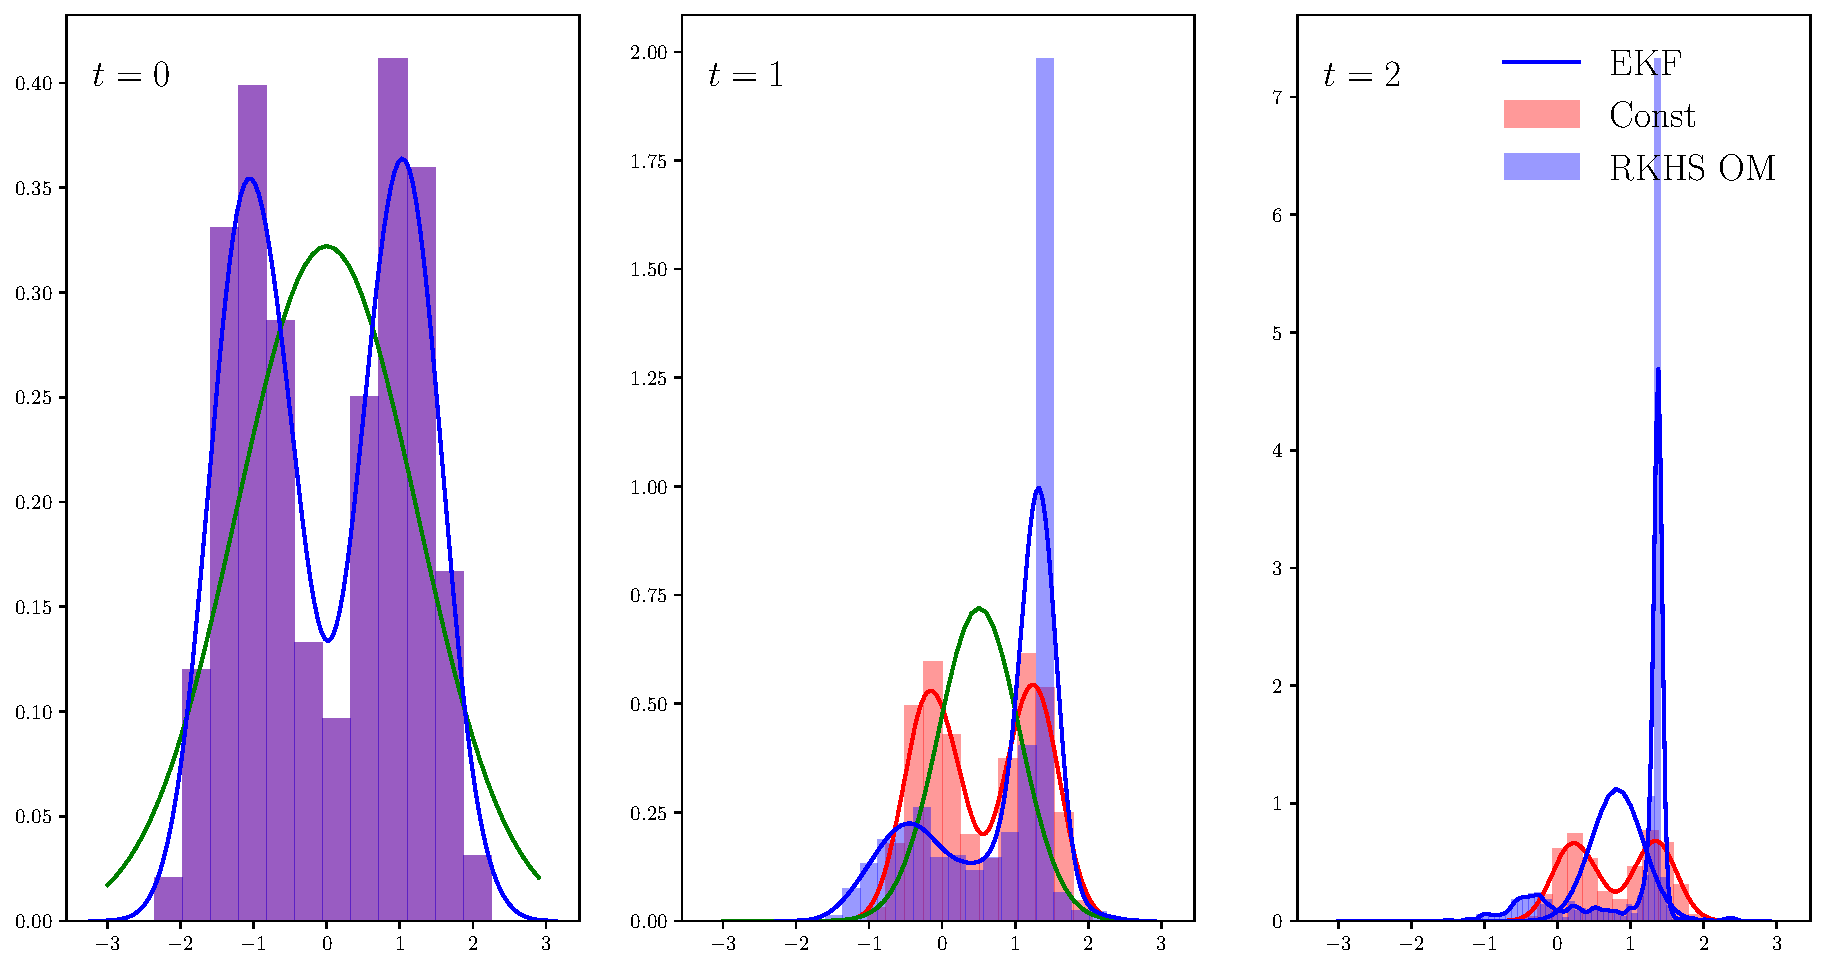
\includegraphics[width = 6in] {images/Chap4_Posterior_estimate}
	\caption{ Posterior estimates $\pr_t^{(N)}$ using EKF, FPF with constant gain and FPF with $\gradTD$-RKHS-OM gain approximations at i) $t=0$ ,ii) $t = 50$, iii) $t = 100$}
	\label{fig:gain_hist_028}
\end{figure}


%The four plots in \Fig{fig:gain_hist_028}  display  gain approximations and posterior approximations for times $t = 0,1$ and $2$.   The results were  obtained using three gain algorithms:  RKHS-OM with and without memory, and  the exact gain.  The parameter
%$\lambda_1$ was set to $1$ in these experiments. The estimates of the posterior obtained using EM match the histograms of the particles using either FPF implementation.

\Fig{steady_state_estimate} displays the trajectories of the state estimates (obtained as the conditional mean) in a typical run.  The RKHS-OM implementations perform better than the other algorithms in most experiments. Although the RKHS-OM estimates show fluctuations in the beginning, they tend to closely track the FPF estimates obtained using the exact gain later on. The constant gain FPF implementation shows a slower response and its estimates match the EKF estimates towards the end. The SIS-PF suffers from particle degeneracy midway through the simulation, and hence estimates show almost no change towards the end.

\begin{figure}[htbp]
	\centering
	\Ebox{0.8}{images/Chap4_param_est_state_comparison}
	\caption{ State estimate trajectories from the various filters}
	\label{steady_state_estimate}
\end{figure}

The conditional mean is a crude indicator of success. The goal of this paper is to estimate the entire posterior density for each $t$.

\Fig{histogram_state_estimate} shows the estimates of the posterior density $\pr_t$ obtained at $t=1$ for each implementation.  In the FPF versions run using the exact gain and RKHS-OM methods, $\pr_t$ evolves to a unimodal density. Both estimates have a sharp spike close to the state value $X_t \equiv 1$. The histogram for the constant gain FPF shows bimodal behavior at $t=1$.  The state covariances of the EKF and the constant gain implementation are similar and much larger than the others. In conclusion, the RKHS methods provide   significantly better posterior estimates.

%\begin{figure}[ht]
%	\centering
%	\Ebox{0.9}{images/Chap4_param_est_posterior_comparison}
%	\caption {Posterior estimates $\pr_t$ at $t=1$ from the various filters}
%	\label{histogram_state_estimate}
%\end{figure}

\subsection{Ship dynamics example} 
\label{s:ship_dynamics}
The performance of the FPF was tested for a nonlinear multidimensional dynamical system. This example, originally described in \cite{budchelee07}, has been tested with the constant gain implementation of the FPF in \cite{tilghiomeh13}.

The model  \eqref{e:fpf_ship_dynamics}
underlying this example  describes the motion of a ship in two dimensions.  It has
a constant radial and angular velocity when the ship is within a certain distance from the origin.  Outside of this region, a
restoring force pushes it back towards the origin. The two dimensional state process is modeled by the SDE
\begin{equation}
\begin{aligned}
\rmd X_{t,1} & = - X_{t,2} \rmd t + a_1(X_{t,1}, X_{t,2}) \rmd t + \sigma_1 \rmd B_{t ,1}\\
\rmd X_{t,2} & = X_{t,1} \rmd t + a_2(X_{t,1}, X_{t,2}) \rmd t + \sigma_2 \rmd B_{t,2}
\label{e:fpf_ship_dynamics}
\end{aligned}
\end{equation}
where $\{B_{t,1}\}$ and $\{B_{t,2}\}$ are independent standard Brownian motions, $\sigma_1$ and $\sigma_2$ are constants,
\[
\begin{aligned}
a_i(x) & \eqdef \varsigma \frac{x_i}{|x|^2} - \Theta \frac{x_i}{|x|}\mathbf{1}_{(\varrho,\infty)}(|x|),\\
x & = [x_1\,\, x_2]^\transpose \in \Re^2, \quad i=1,2,
\end{aligned}
\]
where $|x| = \sqrt{x_1^2 + x_2^2}$, and
$\mathbf{1}_{(\varrho,\infty)}$ denotes the indicator function for the set $(\varrho, \infty)$. The parameter values are chosen to be $\varsigma = 2, \Theta  = 50, \varrho = 9$ and $\sigma_1=\sigma_2=0.4$ as in \cite{budchelee07,tilghiomeh13}.

A discrete time observation model is used in \cite{budchelee07}, which may be regarded as an approximation of the
SDE
\[
\ud Z_t = c(X_t)\ud t + \ud W_t,\qquad   c(x) = \arctan(x_2/x_1)\, .
\]
In the experiments that follow, the SDE is approximated using the same sampling time $\delta =0.05$ that is used in  \cite{budchelee07}, so the setup is unchanged.   The value $\sigma_W =2.5$ was used, which is consistent with prior work.
As always, the state disturbance, measurement noise,  and FPF initial conditions were taken to be mutually independent.

%\begin{equation}
%Y_t = c(X_t) + \sigma_V V_t, \qquad t = n \delta, n \geq 0,
%\end{equation}

As in \cite{budchelee07,tilghiomeh13}, 100 independent trials were performed for an overall run time of $8.25s$ each,
with each trial driven by independent process and measurement noise. For each of the 100 trials, the initial state $x_0$ was set to $(0.5 \, , -0.5)^\transpose$.

Two different priors were compared in these experiments, determined by matrices $\Sigma_1 = I_{2\times 2}$ and $ \Sigma_2 = 5 I_{2\times2}$:   filters were initialized with Gaussian prior $N(x_0, \Sigma_i)$ for $i=1,2$. For the particle-based methods, $500$ particles were drawn independently from the prior density. The sequential importance sampling (SIS) particle filter was implemented with deterministic resampling at every third time instant.  For the RKHS based methods, $\lambda = 10^{-1}$ and $\epsy = 2$ were chosen. Exact computation of the gain requires solving a PDE in two dimensions and is omitted here.

\begin{figure}[htbp]
   \centering
	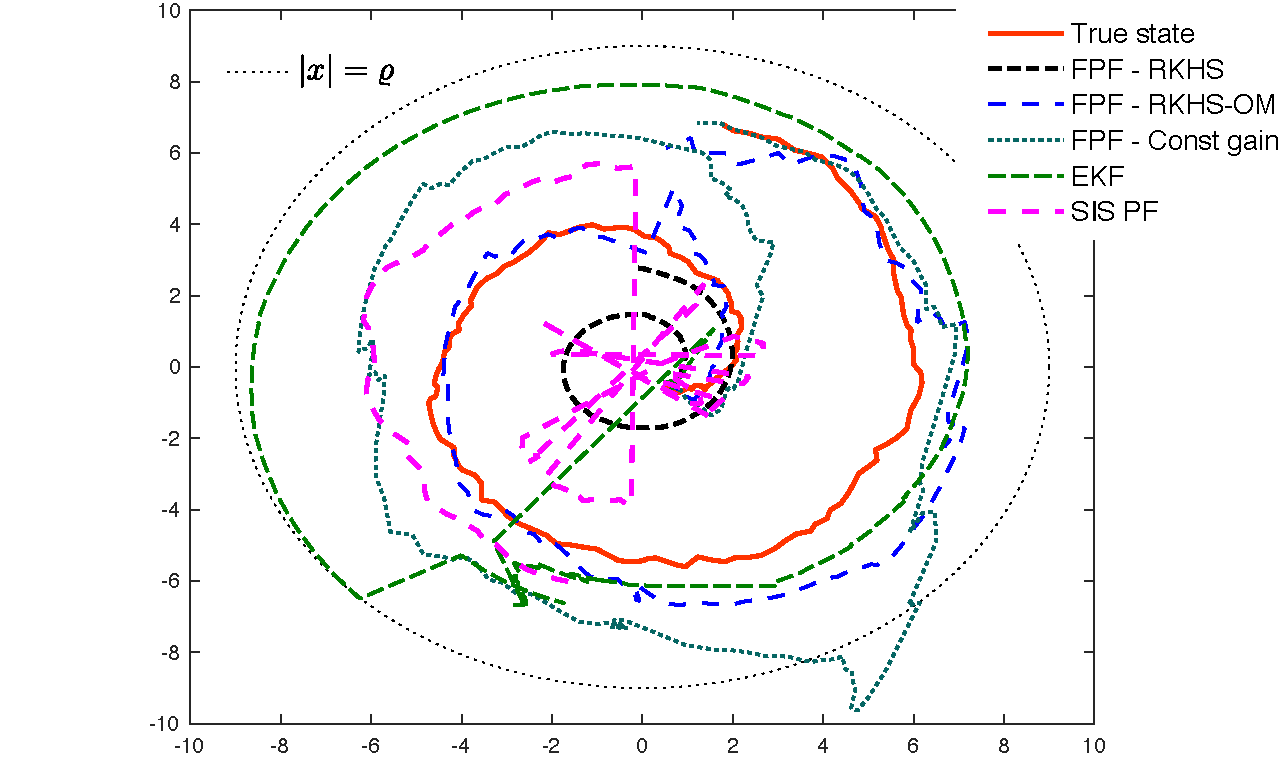
\includegraphics[width=6in]{images/Chap4_ship_state_comparison}
	\caption{Ship trajectory estimates in phase space.}
	\label{fig:ship_state_estimate}
\end{figure}
\begin{figure}[htbp]
	
	\centering
	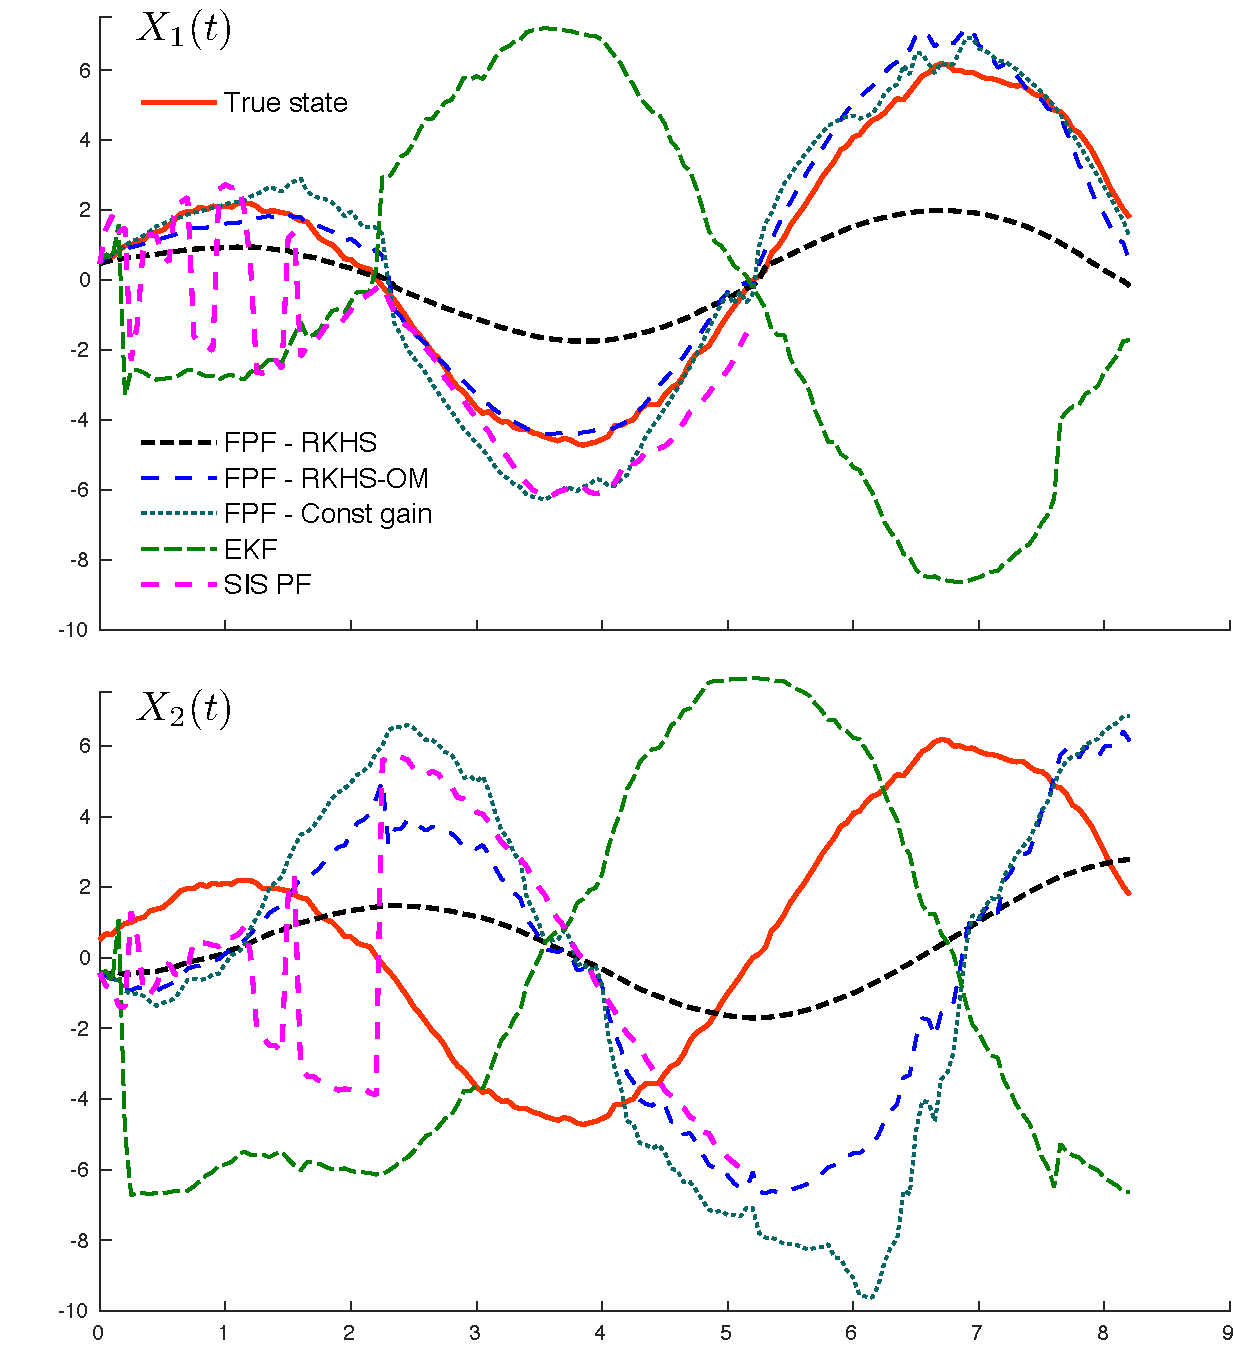
\includegraphics[width =6in] {images/Chap4_ship_state12_comparison}
	\label{fig:ship_state_time_estimate}
	\caption{ State estimates $X_1$ and $X_2$ from the various filters}
\end{figure}

\Fig{fig:ship_state_estimate} displays a typical state trajectory along with the estimates obtained using the each of the five filters using  $\Sigma_2$. The EKF estimates are erratic as reported in \cite{budchelee07}, and are often seen to diverge. The particle methods exhibit superior performance.

The phase-space plot masks the significant delay observed in these experiments.   Individual state estimates for $X_{1}$ and $X_2$ are shown in \Fig{fig:ship_state_time_estimate}.
Estimates of $X_1$ closely follow the actual state trajectory, whereas estimates of the second state  show  significant phase lag. The FPF-RKHS method without the optimal mean is seen to perform poorly. The SIS PF estimates show large fluctuations.
The FPF RKHS-OM method provides the most reliable estimates.

The root-mean-square-error (RMSE) over $100$ independent trials was used to compare the approaches:
\[
\text{RMSE} \eqdef \frac{1}{100} \frac{1}{165} \sum_{j=1}^{100}\sum_{n=1}^{165} | X^j(n \delta) - \hat{X}^j(n \delta) |
\]
where $X^j, \, j= 1 ,\cdots, 100$ represents the signal trajectory, $X^j(n\delta)$ is the true state at time $n\delta$, $\hat{X}^j(n\delta)$ is the state estimate obtained as the conditional mean and $165$ is the total number of time instances for each simulation. Table \ref{table:fpf_rmse} summarizes the results obtained.

The FPF-RKHS-OM provides the lowest RMSE value among the four filters. The EKF performs the worst as the estimates tend to diverge from the true state trajectory in many runs.

Another metric discussed in \cite{budchelee07} is the number of times each filter ``loses its track''. This is obtained by setting a maximum tolerance value for the norm of the estimation error at each instant. If at any instant, the filter estimates produce larger than this tolerance limit, it is considered as having ``lost the track''.   This tolerance limit was set to $10$ in these experiments. The EKF lost track over $93$ times in the $100$ trials, whereas FPF-RKHS-OM lost track only $4$ times.\
\begin{table}[htbp]
	\caption{Comparison of various filters}
		\begin{tabularx}{6.5in}{ XXXX }
			\hline
			Type of filter & $\Sigma_1$ & $\Sigma_2$ & Lost track ($\Sigma_2$) \\
			\hline
			FPF RKHS-OM & $0.9023$  &  $1.6254$ & $4$ times\\
			FPF RKHS mem. &$0.9162$ &  $ 1.9408$ & $ 7 $ times\\
			FPF const. gain & $1.3060$ & $2.3231$ & $14$ times \\
			SIR PF & $3.1481$  &  $4.2648$ &  $57$ times \\
			EKF &  $6.5203$ & $18.441$ & $93$ times \\ 		
			\hline
		\end{tabularx}
		\label{table:fpf_rmse}
\end{table}

\section{Conclusions}
\label{s:ch4_conclusions}
In this Chapter, we introduced the feedback particle filter as an alternate approximation method to nonlinear filtering. Gain approximation is an integral part of this approach to nonlinear filtering. A number of $\gradTD$ learning based gain approximation algorithms were discussed. The generic $\gradTD$ learning scheme is statistically and computationally inefficient as it requires the additional steps of smoothing the posterior density and simulating the Langevin SDE. The $\gradTD$-Langevin algorithm solves some of these issues. The problem of appropriate basis selection which was addressed in \Chapter{ch:rkhs} was illustrated through numerical examples. The RKHS based $\gradTD$ algorithm offers a basis-independent solution and is seen to perform much better than any finite parameterization. This algorithm is also seen to scale easily to higher dimensional systems. The problem of hyperparameter selection in the RKHS methods was also addressed via the RKHS OM method, where the additional information about the constant gain approximation reduces the sensitivity of the solution to the parameters $\epsy$ and $\reg$. For online estimation of the gain in filtering problems, an enhancement that takes into account that the posterior densities and FPF gain evolve with known dynamics was also presented. 

Numerical examples demonstrate the superiority of the RKHS based algorithms over the finite parameterization methods and they are on par with the Markov semigroup approximation method that was developed in parallel research. It is hypothesized that the RKHS based methods offer a more robust and computationally efficient solution, as it avoids the need for successive approximation techniques. In the filtering examples, the FPF implementations with RKHS based gain approximation perform much better than EKF or the constant gain FPF. It also overcomes the resampling and particle degeneracy issues associated with the conventional particle filters. 

There remain many open questions.   Alternatives to the EM algorithm like kernel density estimation must be explored for density approximation based on particles,  and it will be valuable to apply variance reduction techniques to improve the $\nabla$-TD learning algorithms. In terms of mathematical challenges, the most important open problem is robustness of the filter to modeling error, including the impact of an imperfect FPF gain.
